\newpage
\section{Casi d'uso}
Vengono elencati i casi d'uso ricavati dall'analisi del capitolato C1.

\subsection{Attori}
Di seguito è riportato il diagramma UML che descrive la gerarchia degli attori. Sono sono state individuate 3 tipologie differenti di attori con funzionalità crescenti. Gli attori sono: l'utente non autenticato, l'utente autenticato e l'amministratore API Market (un attore autenticato con alcune funzionalità superuser)
\label{Attori}

\begin{figure}[ht]
	\centering
	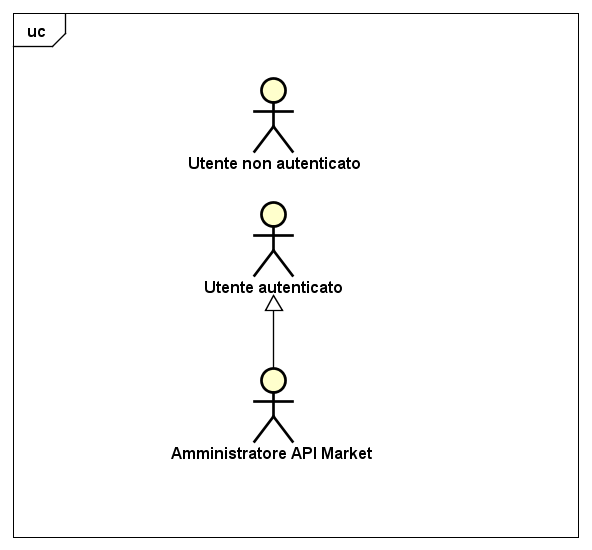
\includegraphics[scale=0.45]{UML/attori.png}
	\caption{Attori}
\end{figure}


\newpage
\subsection{Caso d'uso UC1: Main pre-autenticazione}
\label{UC1}
\begin{figure}[ht]
	\centering
	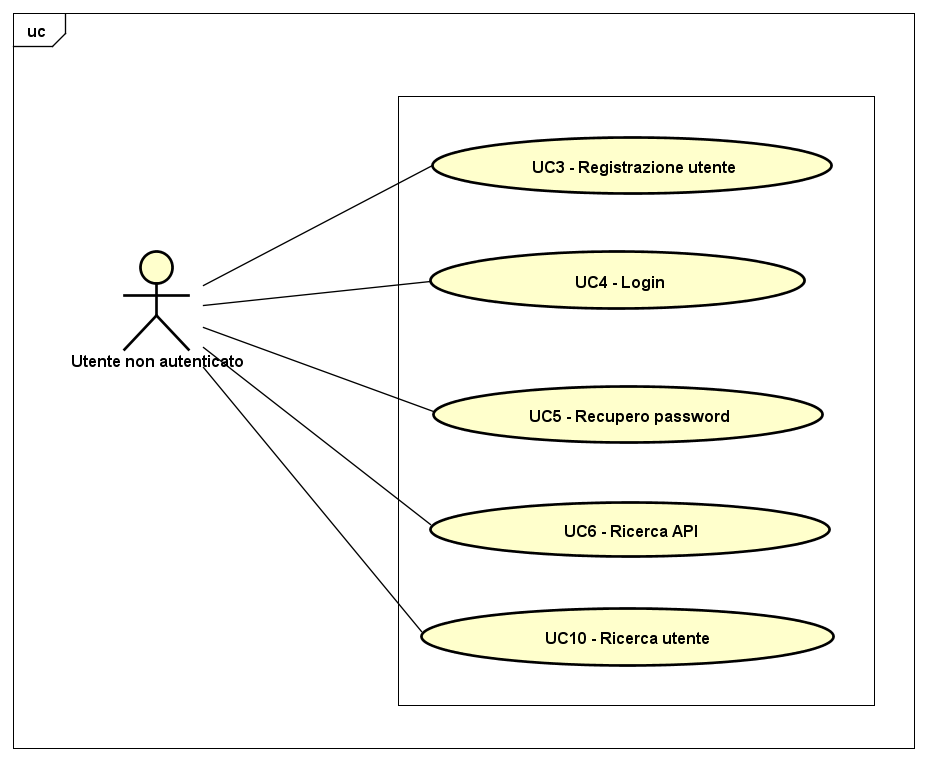
\includegraphics[scale=0.45]{UML/UC1.png}
	\caption{UC1: Main pre-autenticazione}
\end{figure}

\renewcommand*{\arraystretch}{1.6}
\begin{longtable}{ l | p{11cm}}
	\hline
	\rowcolor{Gray}
	\multicolumn{2}{c}{UC1 - Main pre-autenticazione} \\
	\hline
	\textbf{Attori} & Utente non autenticato  \\
	\textbf{Descrizione} & L'attore si trova nella schermata principale dell'applicazione ed accede alle funzionalità a lui disponibili: la registrazione, il login, il recupero password, la ricerca API \\
	\textbf{Pre-Condizioni} & L'attore ha avviato l'applicazione web e non si è ancora autenticato \\
	\textbf{Post-Condizioni} & L'applicazione ha eseguito le richieste dell'attore \\
	\textbf{Scenario Principale} & 
	\begin{enumerate*}[label=(\arabic*.),itemjoin={\newline}]
		\item L'attore può registrarsi all'applicazione (UC3)
		\item L'attore può effettuare il login all'applicazione (UC4)
		\item L'attore può recuperare la propria password (UC5)
		\item L'attore può effettuare una ricerca sulle API presenti nell'applicazione (UC6)
	\end{enumerate*}\\
	\textbf{Scenari Alternativi} & 
	\begin{enumerate*}[label=(\arabic*.),itemjoin={\newline}]
		\item L'attore può effettuare il login tramite API Market (UC4.1)
		\item L'attore può effettuare il login tramite Facebook (UC4.2)
		\item L'attore può effettuare il login tramite Twitter (UC4.3)
		\item L'attore può effettuare il login tramite LinkedIn (UC4.4)
		\item L'attore può effettuare il login tramite Google+ (UC4.5)
	\end{enumerate*}\\
\end{longtable}
\newpage
\subsection{Caso d'uso UC2: Main post-autenticazione }
\label{UC2}
\begin{figure}[ht]
	\centering
	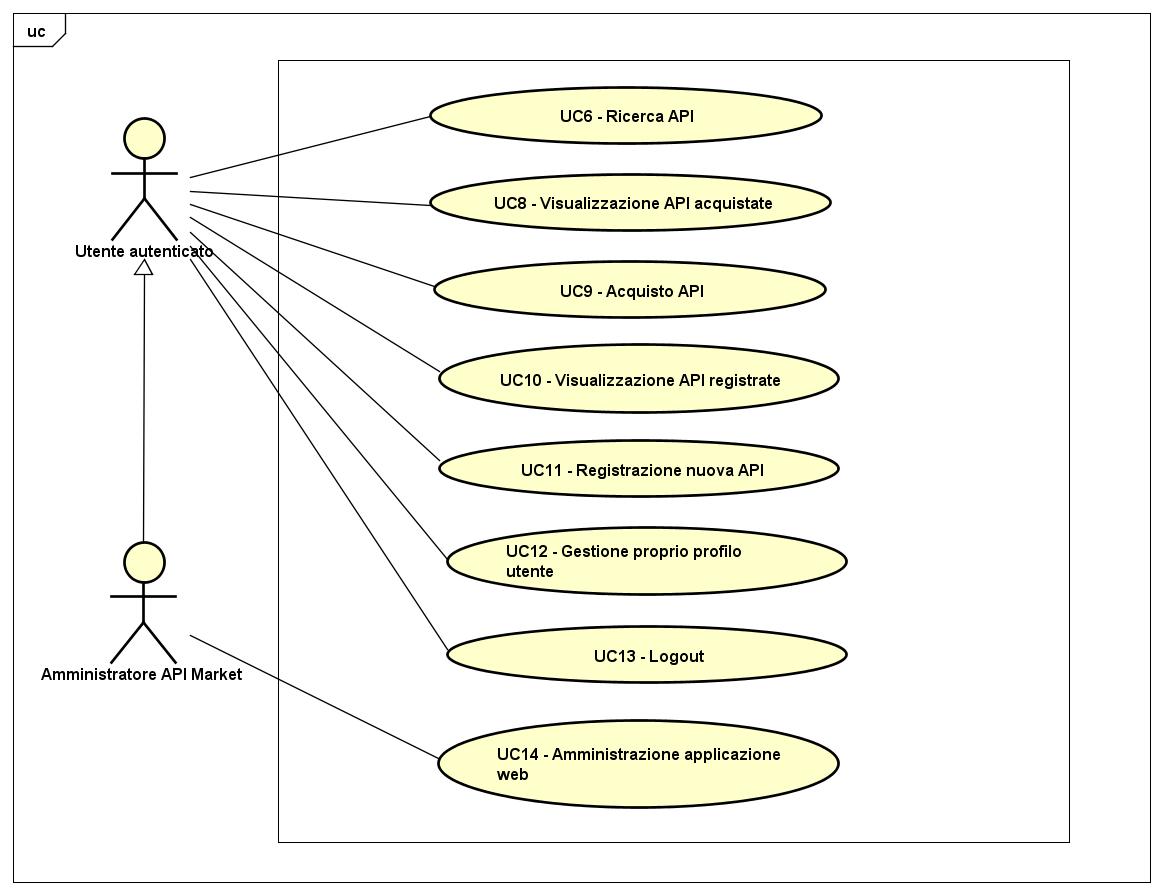
\includegraphics[scale=0.45]{UML/UC2.png}
	\caption{UC2: Main post-autenticazione}
\end{figure}

\begin{longtable}{ l | p{11cm}}
	\hline
	\rowcolor{Gray}
	 \multicolumn{2}{c}{UC2 - Main post-autenticazione} \\
	 \hline
	\textbf{Attori} & Utente autenticato, Amministratore API Market \\
	\textbf{Descrizione} & L'attore tramite la schermata principale
	dell'applicazione, può accedere e sfruttare le funzionalità a lui disponibili: l'interazione
	con il proprio profilo utente, con le API non acquistate e non, con le API registrate, la
	registrazione di una nuova API, il logout. 
	L'Amministratore API Market, oltre alle funzionalità offerte all'utente autenticato, può
	visualizzare i dati di utilizzo delle API ed amministrare l'applicazione web.  \\
	\textbf{Pre-Condizioni} & L'attore ha avviato l'applicazione web e si è autenticato \\
	\textbf{Post-Condizioni} & L'applicazione ha eseguito le richieste dell'attore \\
	\textbf{Scenario Principale} & 
	\begin{enumerate*}[label=(\arabic*.),itemjoin={\newline}]
		\item L'attore può effettuare una ricerca sulle API presenti nell'applicazione
(UC6)
		\item L'attore può visualizzare le API da lui acquistate (UC7)
		\item L'attore può visualizzare le API da lui registrate (UC8)
		\item L'attore può registrare una nuova API (UC9)
		\item L'attore può effettuare una ricerca sugli utenti registrati all'applicazione (UC10)
		\item L'attore può visualizzare il proprio profilo utente (UC11)
		\item L'attore può effettuare il logout (UC12)
		\item L'amministratore API Market può accedere ai servizi di amministrazione dell'applicazione web (UC13)
	\end{enumerate*}\\
\end{longtable}
\newpage
\subsection{Caso d'uso UC3:  Registrazione utente }
\label{UC3}
\begin{figure}[ht]
	\centering
	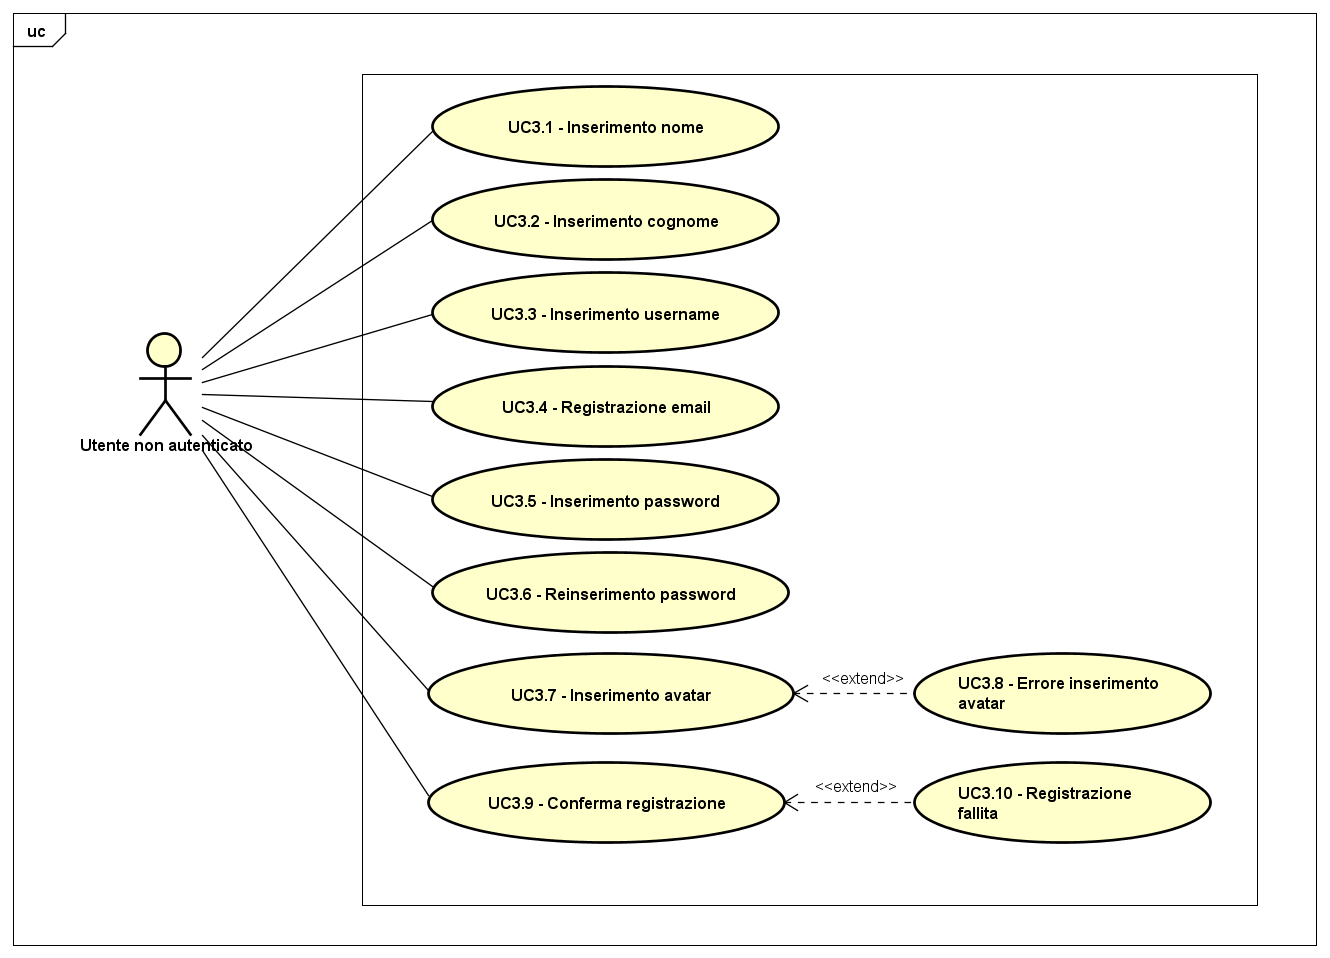
\includegraphics[scale=0.45]{UML/UC3.png}
	\caption{UC3: Registrazione utente}
\end{figure}

\begin{longtable}{ l | p{11cm}}
	\hline
	\rowcolor{Gray}
	 \multicolumn{2}{c}{UC3 - Registrazione utente} \\
	 \hline
	\textbf{Attori} & Utente non autenticato \\
	\textbf{Descrizione} & L'attore inserisce le sue informazioni personali per potersi registrare all'applicazione web, così da poter successivamente effettuare il login ed evolversi in un utente autenticato.
	L'amministratore API Market, oltre alle funzionalità offerte all'utente autenticato, può
	visualizzare i dati di utilizzo delle API ed amministrare l'applicazione web.  \\
	\textbf{Pre-Condizioni} & L'attore ha scelto di registrarsi e l'applicazione web mostra la schermata di registrazione \\
	\textbf{Post-Condizioni} & L'attore si è registrato all'applicazione web \\
	\textbf{Scenario Principale} & \begin{enumerate*}[label=(\arabic*.),itemjoin={\newline}]
		\item L'attore può inserire il proprio nome (UC3.1)
		\item L'attore può inserire il proprio cognome (UC3.2)
		\item L'attore può inserire il proprio username (UC3.3)
		\item L'attore può inserire la propria email (UC3.4) 
		\item L'attore può inserire la propria password (UC3.5)
		\item L'attore può reinserire la propria password per conferma (UC3.6)
		\item L'attore può confermare i dati inseriti, registrandosi all'applicazione web (UC3.7)
	\end{enumerate*}\\
\end{longtable}
\subsubsection{Caso d'uso UC3.1:  Inserimento Nome}
\label{UC3_1}

\begin{longtable}{ l | p{11cm}}
	\hline
	\rowcolor{Gray}
	 \multicolumn{2}{c}{UC3.1 - Inserimento Nome} \\
	 \hline
	\textbf{Attori} & Utente Non Autenticato \\
	\textbf{Descrizione} & L'utente non autenticato inserisce il suo nome  \\
	\textbf{Pre-Condizioni} & L'utente ha scelto di registrarsi e l'applicazione web mostra la schermata di registrazione \\
	\textbf{Post-Condizioni} & L'utente visualizza area per registrazione a applicazione web \\
	\textbf{Scenario Principale} & \begin{enumerate*}[label=(\arabic*.),itemjoin={\newline}]
		\item L'utente non autenticato può inserire il proprio Nome (UC3.1)
	\end{enumerate*}\\
	\textbf{Scenari Alternativi} & 
	\begin{enumerate*}[label=(\arabic*.),itemjoin={\newline}]
		\item Il Nome non e' valido perche' contiene caratteri particolari
	\end{enumerate*}\\
\end{longtable}
\subsubsection{Caso d'uso UC3.2:  Inserimento Cognome}
\label{UC3_2}

\begin{longtable}{ l | p{11cm}}
	\hline
	\rowcolor{Gray}
	 \multicolumn{2}{c}{UC3.2 - Inserimento Cognome} \\
	 \hline
	\textbf{Attori} & Utente Non Autenticato \\
	\textbf{Descrizione} & L'utente non autenticato inserisce il suo Cognome  \\
	\textbf{Pre-Condizioni} & L'utente ha scelto di registrarsi e l'applicazione web mostra la schermata di registrazione \\
	\textbf{Post-Condizioni} & L'utente visualizza area per registrazione a applicazione web \\
	\textbf{Scenario Principale} & \begin{enumerate*}[label=(\arabic*.),itemjoin={\newline}]
		\item L'utente non autenticato può inserire il proprio Cognome (UC3.2)
	\end{enumerate*}\\
	\textbf{Scenari Alternativi} & 
	\begin{enumerate*}[label=(\arabic*.),itemjoin={\newline}]
		\item Il Cognome non e' valido perche' contiene caratteri particolari
	\end{enumerate*}\\
\end{longtable}
\subsubsection{Caso d'uso UC3.3: Inserimento username}
\label{UC3_3}

\begin{longtable}{ l | p{11cm}}
	\hline
	\rowcolor{Gray}
	 \multicolumn{2}{c}{UC3.3: Inserimento username} \\
	 \hline
	\textbf{Attori} & Utente non autenticato \\
	\textbf{Descrizione} & L'attore inserisce lo username desiderato \\
	\textbf{Pre-Condizioni} & L'applicazione mostra il campo dati per l'inserimento dello username \\
	\textbf{Post-Condizioni} & L'attore ha inserito lo username desiderato \\
	\textbf{Scenario Principale} & \begin{enumerate*}[label=(\arabic*.),itemjoin={\newline}]
		\item L'attore può inserire lo username desiderato
	\end{enumerate*}\\
\end{longtable}
\subsubsection{Caso d'uso UC3.4:  Registrazione email}
\label{UC3_4}

\begin{longtable}{ l | p{11cm}}
	\hline
	\rowcolor{Gray}
	 \multicolumn{2}{c}{UC3.4 - Inserimento email} \\
	 \hline
	\textbf{Attori} & Utente non autenticato \\
	\textbf{Descrizione} & L'attore inserisce la propria email  \\
	\textbf{Pre-Condizioni} & L'applicazione visualizza i form per l'inserimento del campo per l'email \\
	\textbf{Post-Condizioni} & L'attore ha inserito la propria email \\
	\textbf{Scenario Principale} & \begin{enumerate*}[label=(\arabic*.),itemjoin={\newline}]
		\item L'utente non autenticato può inserire la propria email
	\end{enumerate*}\\
\end{longtable}

\subsubsection{Caso d'uso UC3.5:  Inserimento Password}
\label{UC3_5}

\begin{longtable}{ l | p{11cm}}
	\hline
	\rowcolor{Gray}
	 \multicolumn{2}{c}{UC3.5 - Inserimento Conferma Password} \\
	 \hline
	\textbf{Attori} & Utente Non Autenticato \\
	\textbf{Descrizione} & L'utente non autenticato inserisce la Password  \\
	\textbf{Pre-Condizioni} & L'utente ha scelto di registrarsi e l'applicazione web mostra la schermata di registrazione \\
	\textbf{Post-Condizioni} & L'utente visualizza area per registrazione a applicazione web \\
	\textbf{Scenario Principale} & \begin{enumerate*}[label=(\arabic*.),itemjoin={\newline}]
		\item L'utente non autenticato può inserire la Password (UC3.5)
	\end{enumerate*}\\
	\textbf{Scenari Alternativi} & 
	\begin{enumerate*}[label=(\arabic*.),itemjoin={\newline}]
		\item La password non e' valida perche' contiene caratteri particolari
		\item La password non e' valida perche' troppo corta
		\item La password non e' valida perche' non contiene almeno un numero
	\end{enumerate*}\\
\end{longtable}
\subsubsection{Caso d'uso UC3.6: Reinserimento password}
\label{UC3_6}

\begin{longtable}{ l | p{11cm}}
	\hline
	\rowcolor{Gray}
	 \multicolumn{2}{c}{UC3.6 - Reinserimento password} \\
	 \hline
	\textbf{Attori} & Utente non autenticato \\
	\textbf{Descrizione} & L'attore reinserisce la password desiderata  \\
	\textbf{Pre-Condizioni} & L'applicazione mostra il campo dati per il reinserimento della password \\
	\textbf{Post-Condizioni} & L'attore ha reinserito la password desiderata \\
	\textbf{Scenario Principale} & \begin{enumerate*}[label=(\arabic*.),itemjoin={\newline}]
		\item L'attore può reinserire la password desiderata
	\end{enumerate*}\\
\end{longtable}
\subsubsection{Caso d'uso UC3.7:  Conferma Inserimenti}
\label{UC3_7}

\begin{longtable}{ l | p{11cm}}
	\hline
	\rowcolor{Gray}
	 \multicolumn{2}{c}{UC3.7 - Conferma Inserimenti} \\
	 \hline
	\textbf{Attori} & Utente Non Autenticato \\
	\textbf{Descrizione} & L'utente non autenticato Conferma i dati inseriti durante la registrazione \\
	\textbf{Pre-Condizioni} & L'utente ha scelto di registrarsi e l'applicazione web mostra la schermata di registrazione \\
	\textbf{Post-Condizioni} & L'utente visualizza un Messaggio di Conferma Registrazione \\
	\textbf{Scenario Principale} & \begin{enumerate*}[label=(\arabic*.),itemjoin={\newline}]
		\item L'utente non autenticato Conferma gli Inserimenti (UC3.7)
	\end{enumerate*}\\
\end{longtable}
\subsubsection{Caso d'uso UC3.8:  Registrazione fallita}
\label{UC3_8}

\begin{longtable}{ l | p{11cm}}
	\hline
	\rowcolor{Gray}
	 \multicolumn{2}{c}{UC3.8 - Registrazione fallita} \\
	 \hline
	\textbf{Attori} & Utente non autenticato \\
	\textbf{Descrizione} & L'attore non si è registrato con successo  \\
	\textbf{Pre-Condizioni} & L'attore ha confermato i dati inseriti \\
	\textbf{Post-Condizioni} & L'attore visualizza i campi dati errati con relativo suggerimento \\
	\textbf{Scenario Principale} & \begin{enumerate*}[label=(\arabic*.),itemjoin={\newline}]
		\item L'attore visualizza i campi dati che non soddisfano i criteri richiesti dalla piattaforma (E.g: Campi dati vuoti, caratteri speciali, username o email già presente etc.)
	\end{enumerate*}\\
\end{longtable}
\newpage
\subsection{Caso d'uso UC4: Login}
\label{UC4}

\begin{longtable}{ l | p{11cm}}
	\hline
	\rowcolor{Gray}
	 \multicolumn{2}{c}{UC4 - Login}\\
	 \hline
	\textbf{Attori} & Utente non autenticato \\
	\textbf{Descrizione} & L'attore inserisce le sue informazioni personali per poter accedere all'applicazione web ed evolversi in un utente autenticato \\
	\textbf{Pre-Condizioni} & L'attore si trova nella schermata iniziale dell'applicazione web \\
	\textbf{Post-Condizioni} & L'attore ha effettuato l'accesso all'applicazione web \\
	\textbf{Scenario Principale} & 
	\begin{enumerate*}[label=(\arabic*.),itemjoin={\newline}]
		\item L'attore può effettuare il login all'applicazione web
	\end{enumerate*}\\
\end{longtable}
\subsubsection{Caso d'uso UC4.1:  Login Base}
\label{UC4_1}
\begin{figure}[ht]
	\centering
	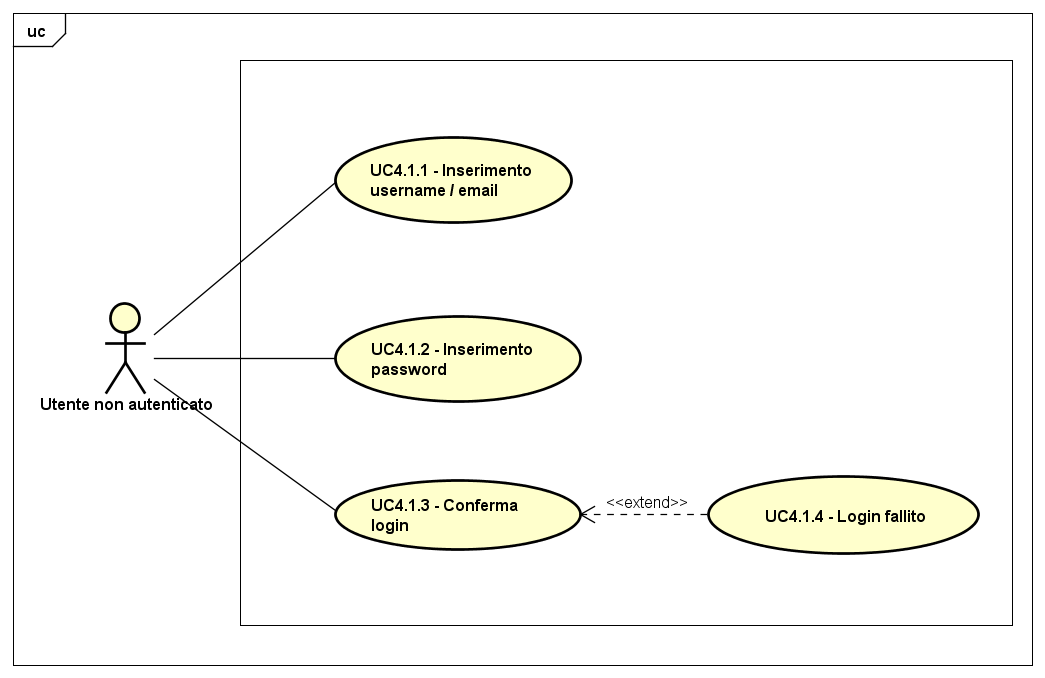
\includegraphics[scale=0.45]{UML/UC4_1.png}
	\caption{UC4.1: Login Base}
\end{figure}

\begin{tabular}{ l | p{11cm}}
	\hline
	\rowcolor{Gray}
	 \multicolumn{2}{c}{UC4.1 - Login Base} \\
	 \hline
	\textbf{Attori} & Utente Non Autenticato \\
	\textbf{Descrizione} & L'utente non autenticato effettua il login all'applicazione web, così da evolversi in un utente autenticato\\
	\textbf{Pre-Condizioni} & L'utente ha scelto di eseguire il login all'applicazione web e non è autenticato \\
	\textbf{Post-Condizioni} & L'utente ha effettuato il login all'applicazione web, evolvendosi in un utente autenticato \\
	\textbf{Scenario Principale} & 
	\begin{enumerate*}[label=(\arabic*.),itemjoin={\newline}]
		\item L'utente non autenticato può inserire l'email o username(UC4.1.1)
		\item L'utente non autenticato può inserire la password(UC4.1.2)
		\item L'utente non autenticato può confermare i dati per loggarsi(UC4.1.3)
	\end{enumerate*}\\
		\textbf{Scenari Alternativi} & 
	\begin{enumerate*}[label=(\arabic*.),itemjoin={\newline}]
		\item L'utente non autenticato visualizza un errore dovuto a un mismatch dei dati immessi e il login non avviene (UC4.1.4)
	\end{enumerate*}\\
\end{tabular}
\subsubsection{Caso d'uso UC4.2:  Login Tramite Facebook }
\label{UC4_2}
\begin{figure}[ht]
	\centering
	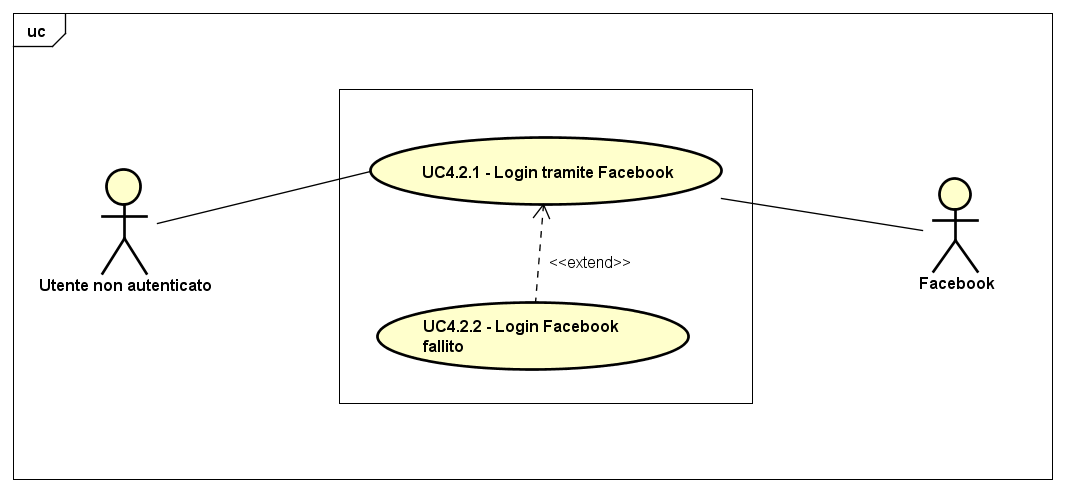
\includegraphics[scale=0.45]{UML/UC4_2.png}
	\caption{UC4.2: Login Tramite Facebook}
\end{figure}

\begin{tabular}{ l | p{11cm}}
	\hline
	\rowcolor{Gray}
	 \multicolumn{2}{c}{UC4.2 - Login Tramite Facebook} \\
	 \hline
	\textbf{Attori} & Utente Non Autenticato, Facebook \\
	\textbf{Descrizione} & L'utente non autenticato effettua il login all'applicazione web tramite Facebook, così da evolversi in un utente autenticato\\
	\textbf{Pre-Condizioni} & L'utente ha scelto di eseguire il login all'applicazione web e non è autenticato \\
	\textbf{Post-Condizioni} & L'utente ha effettuato il login all'applicazione web tramite Facebook, evolvendosi in un utente autenticato \\
	\textbf{Scenario Principale} & \begin{enumerate*}[label=(\arabic*.),itemjoin={\newline}]
		\item L'utente non autenticato può effettuare il login all'applicazione web tramite Facebook (UC4.2.1)
	\end{enumerate*}\\
\end{tabular}
\newpage
\subsubsection{Caso d'uso UC4.3: Login tramite Twitter }
\label{UC4_3}
\begin{figure}[!htbp]
	\centering
	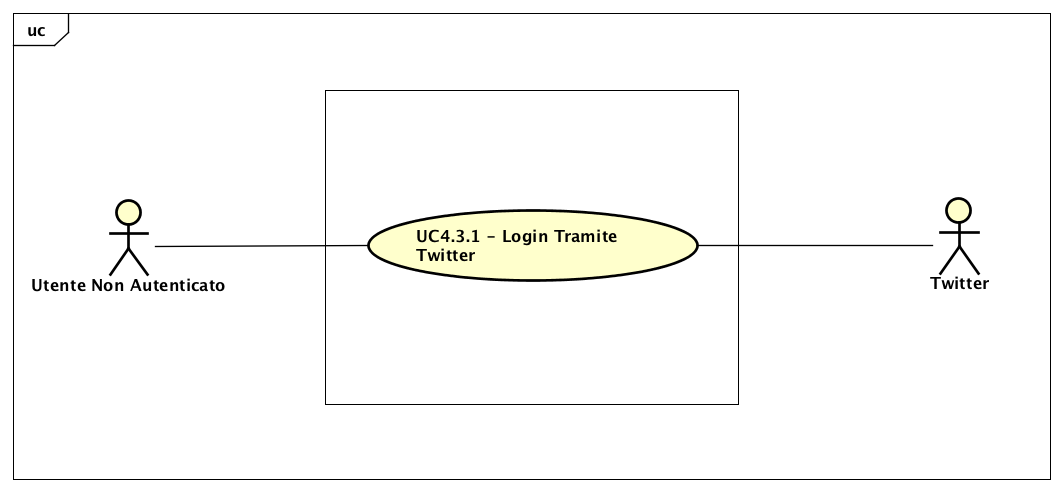
\includegraphics[scale=0.45]{UML/UC4_3.png}
	\caption{UC4.3: Login tramite Twitter}
\end{figure}

\begin{tabular}{ l | p{11cm}}
	\hline
	\rowcolor{Gray}
	\multicolumn{2}{c}{UC4.3 - Login tramite Twitter} \\
	\hline
	\textbf{Attori} & Utente non autenticato, Twitter \\
	\textbf{Descrizione} & L'attore effettua il login all'applicazione web tramite Twitter, così da evolversi in un utente autenticato \\
	\textbf{Pre-Condizioni} & L'attore ha scelto di eseguire il login all'applicazione web tramite Twitter (e non è autenticato) \\
	\textbf{Post-Condizioni} & L'attore ha effettuato il login all'applicazione web tramite Twitter, evolvendosi in un utente autenticato \\
	\textbf{Scenario Principale} & \begin{enumerate*}[label=(\arabic*.),itemjoin={\newline}]
		\item L'attore può effettuare con successo il login tramite Twitter (UC4.3.1), visualizzando un messaggio di successo, e venendo reindirizzato alla pagina principale evolvendosi in un utente autenticato (UC2)
	\end{enumerate*}\\
	\textbf{Scenari Alternativi} & \begin{enumerate*}[label=(\arabic*.),itemjoin={\newline}]
	\item L'attore ha fallito il login tramite Twitter (E.g: Mancanza di privilegi/autorizzazioni, problemi legati a Twitter...) e visualizza un messaggio d'errore (UC4.3.2)
	\end{enumerate*}\\
\end{tabular}
\newpage
\subsubsection{Caso d'uso UC4.4: Login tramite LinkedIn }
\label{UC4_2}
\begin{figure}[!htbp]
	\centering
	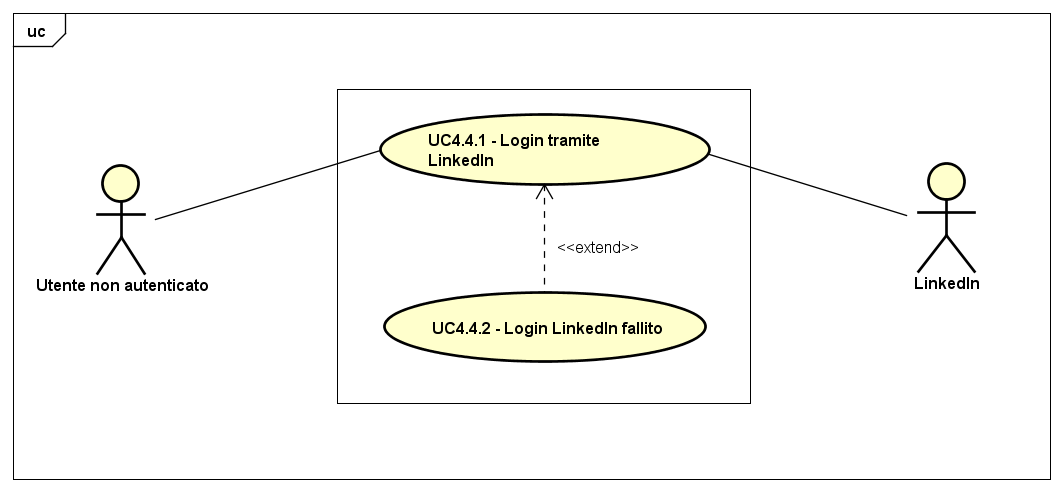
\includegraphics[scale=0.45]{UML/UC4_4.png}
	\caption{UC4.2: Login tramite LinkedIn}
\end{figure}

\begin{tabular}{ l | p{11cm}}
	\hline
	\rowcolor{Gray}
	\multicolumn{2}{c}{UC4.4 - Login tramite LinkedIn} \\
	\hline
	\textbf{Attori} & Utente non autenticato, LinkedIn \\
	\textbf{Descrizione} & L'attore effettua il login all'applicazione web tramite LinkedIn, così da evolversi in un utente autenticato \\
	\textbf{Pre-Condizioni} & L'attore ha scelto di eseguire il login all'applicazione web tramite LinkedIn (e non è autenticato) \\
	\textbf{Post-Condizioni} & L'attore ha effettuato il login all'applicazione web tramite LinkedIn, evolvendosi in un utente autenticato \\
	\textbf{Scenario Principale} & \begin{enumerate*}[label=(\arabic*.),itemjoin={\newline}]
		\item L'attore può effettuare con successo il login tramite LinkedIn (UC4.4.1), visualizzando un messaggio di successo, e venendo reindirizzato alla pagina principale evolvendosi in un utente autenticato (UC2)
	\end{enumerate*}\\
	\textbf{Scenari Alternativi} & \begin{enumerate*}[label=(\arabic*.),itemjoin={\newline}]
	\item L'attore ha fallito il login tramite LinkedIn (E.g: Mancanza di privilegi/autorizzazioni, utente non correttamente loggato a LinkedIn...) e visualizza un messaggio d'errore (UC4.4.2)
	\end{enumerate*}\\
\end{tabular}

\subsubsection{Caso d'uso UC4.5: Login Tramite Google+ }
\label{UC4_5}
\begin{figure}[ht]
	\centering
	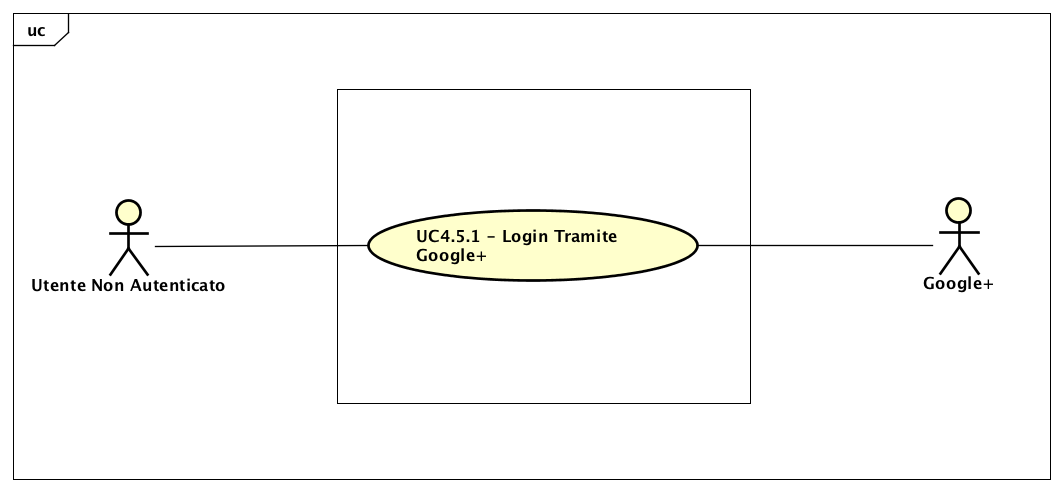
\includegraphics[scale=0.45]{UML/UC4_5.png}
	\caption{UC4.5: Login Tramite Google+ }
\end{figure}

\begin{longtable}{ l | p{11cm}}
	\hline
	\rowcolor{Gray}
	 \multicolumn{2}{c}{UC4.5 - Login Tramite Google+} \\
	 \hline
	\textbf{Attori} & Utente Non Autenticato, Google+ \\
	\textbf{Descrizione} & L'utente non autenticato effettua il login all'applicazione web tramite Google+, così da evolversi in un utente autenticato\\
	\textbf{Pre-Condizioni} & L'utente ha scelto di eseguire il login all'applicazione web e non è autenticato \\
	\textbf{Post-Condizioni} & L'utente ha effettuato il login all'applicazione web tramite Google+, evolvendosi in un utente autenticato\\
	\textbf{Scenario Principale} & \begin{enumerate*}[label=(\arabic*.),itemjoin={\newline}]
		\item L'utente non autenticato può effettuare il login all'applicazione web tramite Google+ (UC4.5.1)
	\end{enumerate*}\\
\end{longtable}
\newpage
\subsection{Caso d'uso UC5: Recupero password}
\label{UC5}
\begin{figure}[ht]
	\centering
	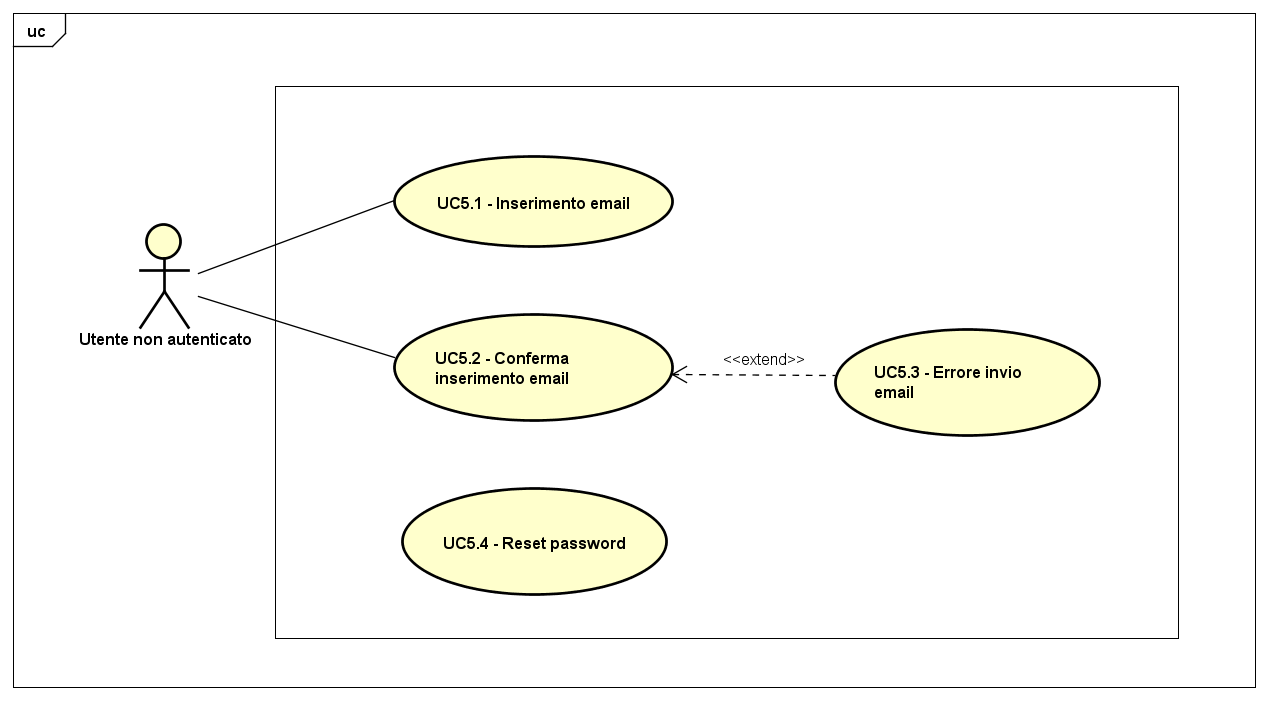
\includegraphics[scale=0.45]{UML/UC5.png}
	\caption{UC5: Recupero password}
\end{figure}

\begin{longtable}{ l | p{11cm}}
	\hline
	\rowcolor{Gray}
	 \multicolumn{2}{c}{UC5 - Recupero password} \\
	 \hline
	\textbf{Attori} & Utente non autenticato \\
	\textbf{Descrizione} & L'attore recupera la password del proprio account API Market tramite l'invio di una email \\
	\textbf{Pre-Condizioni} & L'attore ha scelto di recuperare la password del proprio account API Market \\
	\textbf{Post-Condizioni} & L'attore ha ricevuto nella propria casella email un link per resettare la password del proprio account API Market, oppure la procedura è fallita \\
	\textbf{Scenario Principale} & 
	\begin{enumerate*}[label=(\arabic*.),itemjoin={\newline}]
		\item L'attore può inserire la propria email (UC5.1)
		\item L'attore può confermare l'indirizzo email inserito, al quale l'applicazione web invierà un link per resettare la password (UC5.2)
	\end{enumerate*}\\
	\textbf{Scenari Alternativi} & 
	\begin{enumerate*}[label=(\arabic*.),itemjoin={\newline}]
		\item L'attore, se ha inserito un'email non valida o inesistente, può visualizzare un messaggio d'errore e l'email di reset password non viene inviata (UC5.3)
		\item L'attore, se ha richiesto il recupero della password ed ha aperto il link per poterla resettare, può effettuare il reset password in una apposita schermata (UC5.4)
	\end{enumerate*}\\
\end{longtable}
\subsubsection{Caso d'uso UC5.1: Inserimento email}
\label{UC5_1}

\begin{minipage}{\linewidth}
\begin{longtable}{ l | p{11cm}}
	\hline
	\rowcolor{Gray}
	 \multicolumn{2}{c}{UC5.1 - Inserimento email} \\
	 \hline
	\textbf{Attori} & Utente non autenticato \\
	\textbf{Descrizione} & L'attore inserisce la sua email  \\
	\textbf{Pre-Condizioni} & L'attore ha dimenticato la password e l'applicazione web mostra la schermata di recupero password\\
	\textbf{Post-Condizioni} & L'attore ha inserito l'email relativa all'account che desidera recuperare\\
	\textbf{Scenario Principale} & \begin{enumerate*}[label=(\arabic*.),itemjoin={\newline}]
		\item L'attore può inserire la propria email (UC5.1)
	\end{enumerate*}\\
\end{longtable}
\end{minipage}
\subsubsection{Caso d'uso UC5.2: Conferma inserimento email}
\label{UC5_2}

\begin{minipage}{\linewidth}
\begin{longtable}{ l | p{11cm}}
	\hline
	\rowcolor{Gray}
	 \multicolumn{2}{c}{UC5.2 - Conferma inserimento email} \\
	 \hline
	\textbf{Attori} & Utente non autenticato \\
	\textbf{Descrizione} & L'attore conferma l'inserimento del proprio indirizzo email tramite un apposito pulsante \\
	\textbf{Pre-Condizioni} & L'attore ha inserito l'email dell'account che intende recuperare\\
	\textbf{Post-Condizioni} & L'attore ha compilato il campo email, relativo all'account che desidera recuperare\\
	\textbf{Scenario Principale} & \begin{enumerate*}[label=(\arabic*.),itemjoin={\newline}]
		\item L'attore può confermare i dati immessi, visualizzando un messaggio di successo e ricevendo tramite email la procedura di recupero password (UC5.4) e viene reindirizzato alla schermata principale (UC1)
	\end{enumerate*}\\
	\textbf{Scenari Alternativi} & 
	\begin{enumerate*}[label=(\arabic*.),itemjoin={\newline}]
		\item L'attore ha inserito un email non valida o inesistente, e visualizza un messaggio d'errore (UC5.3)
	\end{enumerate*}\\
\end{longtable}
\end{minipage}
\subsubsection{Caso d'uso UC5.3: Errore invio email}
\label{UC5_3}

\begin{minipage}{\linewidth}
\begin{longtable}{ l | p{11cm}}
	\hline
	\rowcolor{Gray}
	 \multicolumn{2}{c}{UC5.3 - Errore invio email} \\
	 \hline
	\textbf{Attori} & Utente non autenticato \\
	\textbf{Descrizione} & L'attore riceve un messaggio di errore dovuto all'inserimento di un'email non valida o inesistente \\
	\textbf{Pre-Condizioni} & L'attore ha dimenticato la password e ha inserito l'email per poterla recuperare \\
	\textbf{Post-Condizioni} & L'attore riceve un messaggio di errore e può eventualmente ripetere la procedura di recupero password \\
	\textbf{Scenario Principale} & \begin{enumerate*}[label=(\arabic*.),itemjoin={\newline}]
		\item L'attore visualizza un messaggio d'errore per aver lasciato il campo vuoto o per aver inserito un indirizzo inesistente. Può ripetere la procedura (UC5)
	\end{enumerate*}\\
\end{longtable}
\end{minipage}

\newpage
\subsection{Caso d'uso UC6: Ricerca API}
\label{UC6}
\begin{figure}[ht]
	\centering
	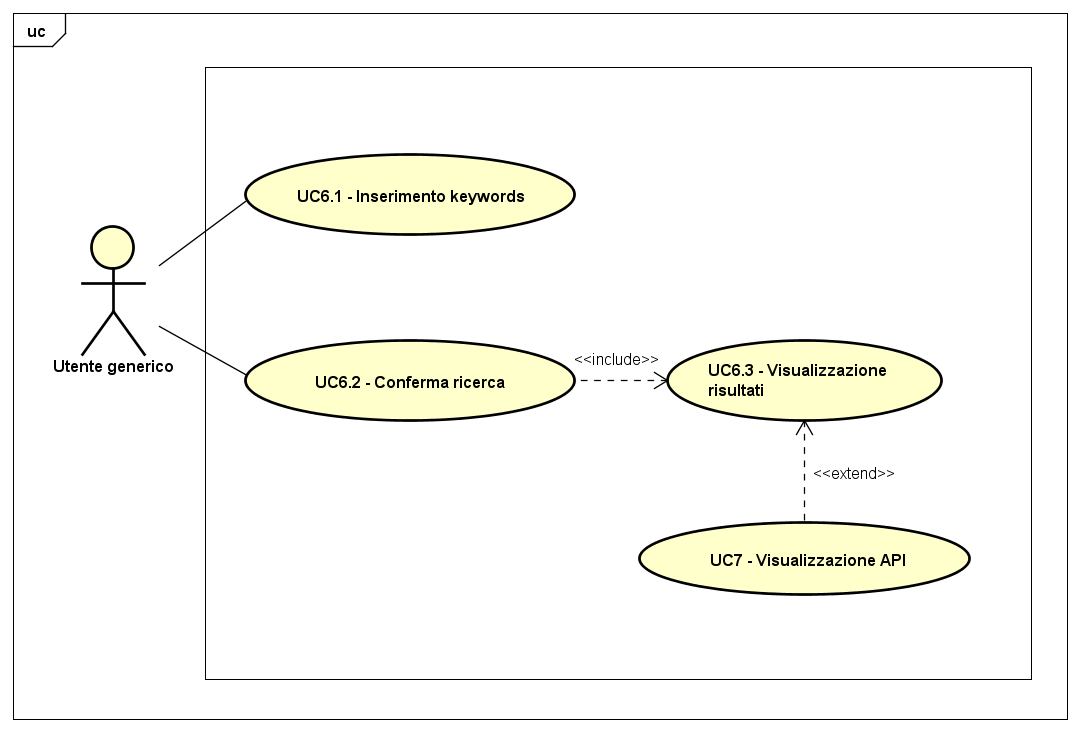
\includegraphics[scale=0.45]{UML/UC6.png}
	\caption{UC6: Ricerca API}
\end{figure}

\begin{longtable}{ l | p{11cm}}
	\hline
	\rowcolor{Gray}
	 \multicolumn{2}{c}{UC6 - Ricerca API} \\
	 \hline
	\textbf{Attori} & Utente generico \\
	\textbf{Descrizione} & L'attore inserisce le keywords per la ricerca di API \\
	\textbf{Pre-Condizioni} & L'attore ha scelto di effettuare una ricerca di API \\
	\textbf{Post-Condizioni} & L'attore ha effettuato la ricerca di API ed ha visualizzato la lista dei risultati \\
	\textbf{Scenario Principale} & 
	\begin{enumerate*}[label=(\arabic*.),itemjoin={\newline}]
		\item L'attore può inserire la stringa di ricerca desiderata (UC6.1)
		\item L'attore può confermare i dati inseriti (UC6.2) e visualizzare i risultati forniti dall'applicazione web (UC6.3)
	\end{enumerate*}\\
\end{longtable}

\subsubsection{Caso d'uso UC6.1: Inserimento keywords}
\label{UC6_1}

\begin{minipage}{\linewidth}
\begin{tabular}{ l | p{11cm}}
	\hline
	\rowcolor{Gray}
	 \multicolumn{2}{c}{UC6.1 - Inserimento keywords} \\
	 \hline
	\textbf{Attori} & Utente generico \\
	\textbf{Descrizione} & L'attore effettua una ricerca delle API inserendo nella barra di ricerca una stringa contenente le keywords desiderate \\
	\textbf{Pre-Condizioni} & L'attore ha scelto di effettuare una ricerca di API \\
	\textbf{Post-Condizioni} & L'attore ha inserito nella barra di ricerca una stringa contenente le keywords desiderate \\
	\textbf{Scenario Principale} & 
	\begin{enumerate*}[label=(\arabic*.),itemjoin={\newline}]
		\item L'attore può inserire nella barra di ricerca una stringa con tenente le keywords desiderate: esse verranno ricercate sul nome dell'API, sul nome dell'autore e su eventuali tag
	\end{enumerate*}\\
\end{tabular}
\end{minipage}

\subsubsection{Caso d'uso UC6.2: Conferma ricerca}
\label{UC6_2}

\begin{minipage}{\linewidth}
	\begin{tabular}{ l | p{11cm}}
		\hline
		\rowcolor{Gray}
		\multicolumn{2}{c}{UC6.2 - Conferma ricerca} \\
		\hline
		\textbf{Attori} & Utente generico \\
		\textbf{Descrizione} & L'attore conferma la stringa di ricerca inserita per poter visualizzare i risultati \\
		\textbf{Pre-Condizioni} & L'attore ha inserito una stringa di ricerca \\
		\textbf{Post-Condizioni} & L'attore ha confermato una stringa di ricerca \\
		\textbf{Scenario Principale} & 
		\begin{enumerate*}[label=(\arabic*.),itemjoin={\newline}]
			\item L'attore può confermare una stringa di ricerca, visualizzando la lista dei risultati (UC6.3)
		\end{enumerate*}\\
	\end{tabular}
\end{minipage}

\newpage
\subsubsection{Caso d'uso UC6.3: Visualizzazione lista risultati}
\label{UC6_3}
\begin{figure}[ht]
	\centering
	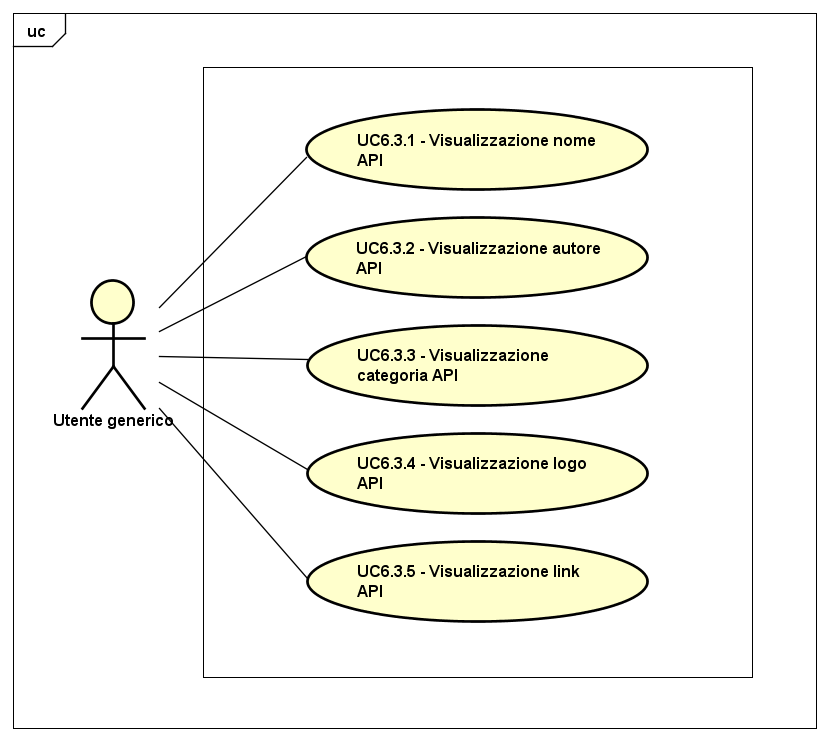
\includegraphics[scale=0.45]{UML/UC6_3.png}
	\caption{UC6.3: Visualizzazione lista risultati}
\end{figure}

\begin{minipage}{\linewidth}
	\begin{tabular}{ l | p{11cm}}
		\hline
		\rowcolor{Gray}
		\multicolumn{2}{c}{UC6.3 - Visualizzazione lista risultati} \\
		\hline
		\textbf{Attori} & Utente generico \\
		\textbf{Descrizione} & L'attore visualizza le API che corrispondono alle keywords della ricerca effettuata \\
		\textbf{Pre-Condizioni} & L'attore ha confermato la ricerca API \\
		\textbf{Post-Condizioni} & L'attore ha visualizzato le API che corrispondono alle keywords della ricerca effettuata \\
		\textbf{Scenario Principale} & 
		\begin{enumerate*}[label=(\arabic*.),itemjoin={\newline}]
			\item L'attore può visualizzare il nome delle API che corrispondono alle keywords della ricerca effettuata (UC6.3.1)
			\
		\end{enumerate*}\\
	\end{tabular}
\end{minipage}

\paragraph{Caso d'uso UC6.3.1: Visualizzazione nome API}
\label{UC6_3_1}

\begin{minipage}{\linewidth}
	\begin{tabular}{ l | p{11cm}}
		\hline
		\rowcolor{Gray}
		\multicolumn{2}{c}{UC6.3.1 - Visualizzazione nome API} \\
		\hline
		\textbf{Attori} & Utente generico \\
		\textbf{Descrizione} & L'attore visualizza nella lista il nome dell'API che corrisponde alle keywords della ricerca effettuata \\
		\textbf{Pre-Condizioni} & L'attore ha confermato la ricerca API \\
		\textbf{Post-Condizioni} & L'attore ha visualizzato nella lista il nome dell'API che corrisponde alle keywords della ricerca effettuata \\
		\textbf{Scenario Principale} & 
		\begin{enumerate*}[label=(\arabic*.),itemjoin={\newline}]
			\item L'attore può visualizzare nella lista il nome dell'API che corrisponde alle keywords della ricerca effettuata
		\end{enumerate*}\\
	\end{tabular}
\end{minipage}

\paragraph{Caso d'uso UC6.3.2: Visualizzazione autore API}
\label{UC6_3_2}

\begin{minipage}{\linewidth}
	\begin{tabular}{ l | p{11cm}}
		\hline
		\rowcolor{Gray}
		\multicolumn{2}{c}{UC6.3.2 - Visualizzazione autore API} \\
		\hline
		\textbf{Attori} & Utente generico \\
		\textbf{Descrizione} & L'attore visualizza nella lista il nome dell'autore dell'API che corrisponde alle keywords della ricerca effettuata \\
		\textbf{Pre-Condizioni} & L'attore ha confermato la ricerca API \\
		\textbf{Post-Condizioni} & L'attore ha visualizzato nella lista il nome dell'autore dell'API che corrisponde alle keywords della ricerca effettuata \\
		\textbf{Scenario Principale} & 
		\begin{enumerate*}[label=(\arabic*.),itemjoin={\newline}]
			\item L'attore può visualizzare nella lista il nome dell'autore dell'API che corrisponde alle keywords della ricerca effettuata
		\end{enumerate*}\\
	\end{tabular}
\end{minipage}

\paragraph{Caso d'uso UC6.3.3: Visualizzazione categoria API}
\label{UC6_3_3}

\begin{minipage}{\linewidth}
	\begin{tabular}{ l | p{11cm}}
		\hline
		\rowcolor{Gray}
		\multicolumn{2}{c}{UC6.3.3 - Visualizzazione categoria API} \\
		\hline
		\textbf{Attori} & Utente generico \\
		\textbf{Descrizione} & L'attore visualizza nella lista la categoria dell'API che corrisponde alle keywords della ricerca effettuata \\
		\textbf{Pre-Condizioni} & L'attore ha confermato la ricerca API \\
		\textbf{Post-Condizioni} & L'attore ha visualizzato nella lista la categoria dell'API che corrisponde alle keywords della ricerca effettuata \\
		\textbf{Scenario Principale} & 
		\begin{enumerate*}[label=(\arabic*.),itemjoin={\newline}]
			\item L'attore può visualizzare nella lista la categoria dell'API che corrisponde alle keywords della ricerca effettuata
		\end{enumerate*}\\
	\end{tabular}
\end{minipage}

\paragraph{Caso d'uso UC6.3.4: Visualizzazione logo API}
\label{UC6_3_4}

\begin{minipage}{\linewidth}
	\begin{tabular}{ l | p{11cm}}
		\hline
		\rowcolor{Gray}
		\multicolumn{2}{c}{UC6.3.4 - Visualizzazione logo API} \\
		\hline
		\textbf{Attori} & Utente generico \\
		\textbf{Descrizione} & L'attore visualizza nella lista il logo dell'API che corrisponde alle keywords della ricerca effettuata \\
		\textbf{Pre-Condizioni} & L'attore ha confermato la ricerca API \\
		\textbf{Post-Condizioni} & L'attore ha visualizzato nella lista il logo dell'API che corrisponde alle keywords della ricerca effettuata \\
		\textbf{Scenario Principale} & 
		\begin{enumerate*}[label=(\arabic*.),itemjoin={\newline}]
			\item L'attore può visualizzare nella lista il logo dell'API che corrisponde alle keywords della ricerca effettuata
		\end{enumerate*}\\
	\end{tabular}
\end{minipage}

\paragraph{Caso d'uso UC6.3.5: Visualizzazione link API}
\label{UC6_3_5}

\begin{minipage}{\linewidth}
	\begin{tabular}{ l | p{11cm}}
		\hline
		\rowcolor{Gray}
		\multicolumn{2}{c}{UC6.3.5 - Visualizzazione link API} \\
		\hline
		\textbf{Attori} & Utente generico \\
		\textbf{Descrizione} & L'attore visualizza nella lista il link alla visualizzazione dell'API che corrisponde alle keywords della ricerca effettuata \\
		\textbf{Pre-Condizioni} & L'attore ha confermato la ricerca API \\
		\textbf{Post-Condizioni} & L'attore ha visualizzato nella lista il link alla visualizzazione dell'API che corrisponde alle keywords della ricerca effettuata \\
		\textbf{Scenario Principale} & 
		\begin{enumerate*}[label=(\arabic*.),itemjoin={\newline}]
			\item L'attore può visualizzare nella lista il link alla visualizzazione dell'API che corrisponde alle keywords della ricerca effettuata, che lo reindirizzerà ad UC7 per l'API in questione
		\end{enumerate*}\\
	\end{tabular}
\end{minipage}
\subsubsection{Caso d'uso UC6.1:  Inserimento Nome API}
\label{UC6_1}

\begin{tabular}{ l | p{11cm}}
	\hline
	\rowcolor{Gray}
	 \multicolumn{2}{c}{UC6.1 - Inserimento Nome API} \\
	 \hline
	\textbf{Attori} & Utente Non Autenticato, Utente Autenticato \\
	\textbf{Descrizione} & Gli utenti possono effettuare una ricerca delle API usandone il nome\\
	\textbf{Pre-Condizioni} & L'utente ha scelto fare una ricerca di API\\
	\textbf{Post-Condizioni} & L'utente ha inserito il nome dell'API nella barra di ricerca \\
	\textbf{Scenario Principale} & 
	\begin{enumerate*}[label=(\arabic*.),itemjoin={\newline}]
		\item L'utente puo' inserire il Nome dell API nella barra di ricerca (UC6.1)
	\end{enumerate*}\\
\end{tabular}
\subsubsection{Caso d'uso UC6.2: Conferma ricerca}
\label{UC6_2}

\begin{minipage}{\linewidth}
	\begin{tabular}{ l | p{11cm}}
		\hline
		\rowcolor{Gray}
		\multicolumn{2}{c}{UC6.2 - Conferma ricerca} \\
		\hline
		\textbf{Attori} & Utente non autenticato, Utente autenticato \\
		\textbf{Descrizione} & L'attore conferma la stringa di ricerca inserita per poter visualizzare i risultati\\
		\textbf{Pre-Condizioni} & L'attore ha inserito una stringa di ricerca\\
		\textbf{Post-Condizioni} & L'attore ha confermato una stringa per la ricerca \\
		\textbf{Scenario Principale} & 
		\begin{enumerate*}[label=(\arabic*.),itemjoin={\newline}]
			\item L'attore può confermare una stringa per la ricerca
		\end{enumerate*}\\
	\end{tabular}
\end{minipage}
\subsubsection{Caso d'uso UC6.3: Visualizza risultati}
\label{UC6_3}

\begin{minipage}{\linewidth}
	\begin{tabular}{ l | p{11cm}}
		\hline
		\rowcolor{Gray}
		\multicolumn{2}{c}{UC6.3 - Visualizza risultati} \\
		\hline
		\textbf{Attori} & Utente non autenticato, Utente autenticato \\
		\textbf{Descrizione} & L'attore visualizza i risultati prodotti dalla piattaforma\\
		\textbf{Pre-Condizioni} & L'attore ha confermato la ricerca\\
		\textbf{Post-Condizioni} & L'attore visualizza i risultati di ricerca prodotti \\
		\textbf{Scenario Principale} & 
		\begin{enumerate*}[label=(\arabic*.),itemjoin={\newline}]
			\item L'attore può visualizzare i risultati della ricerca, che possono essere anche vuoti nel caso di stringhe non consone. L'utente può accedere alla schermata delle singole API (UC7)
		\end{enumerate*}\\
	\end{tabular}
\end{minipage}
\newpage
\subsection{Caso d'uso UC7 - Visualizzazione API}
\label{UC7}
\begin{figure}[ht]
	\centering
	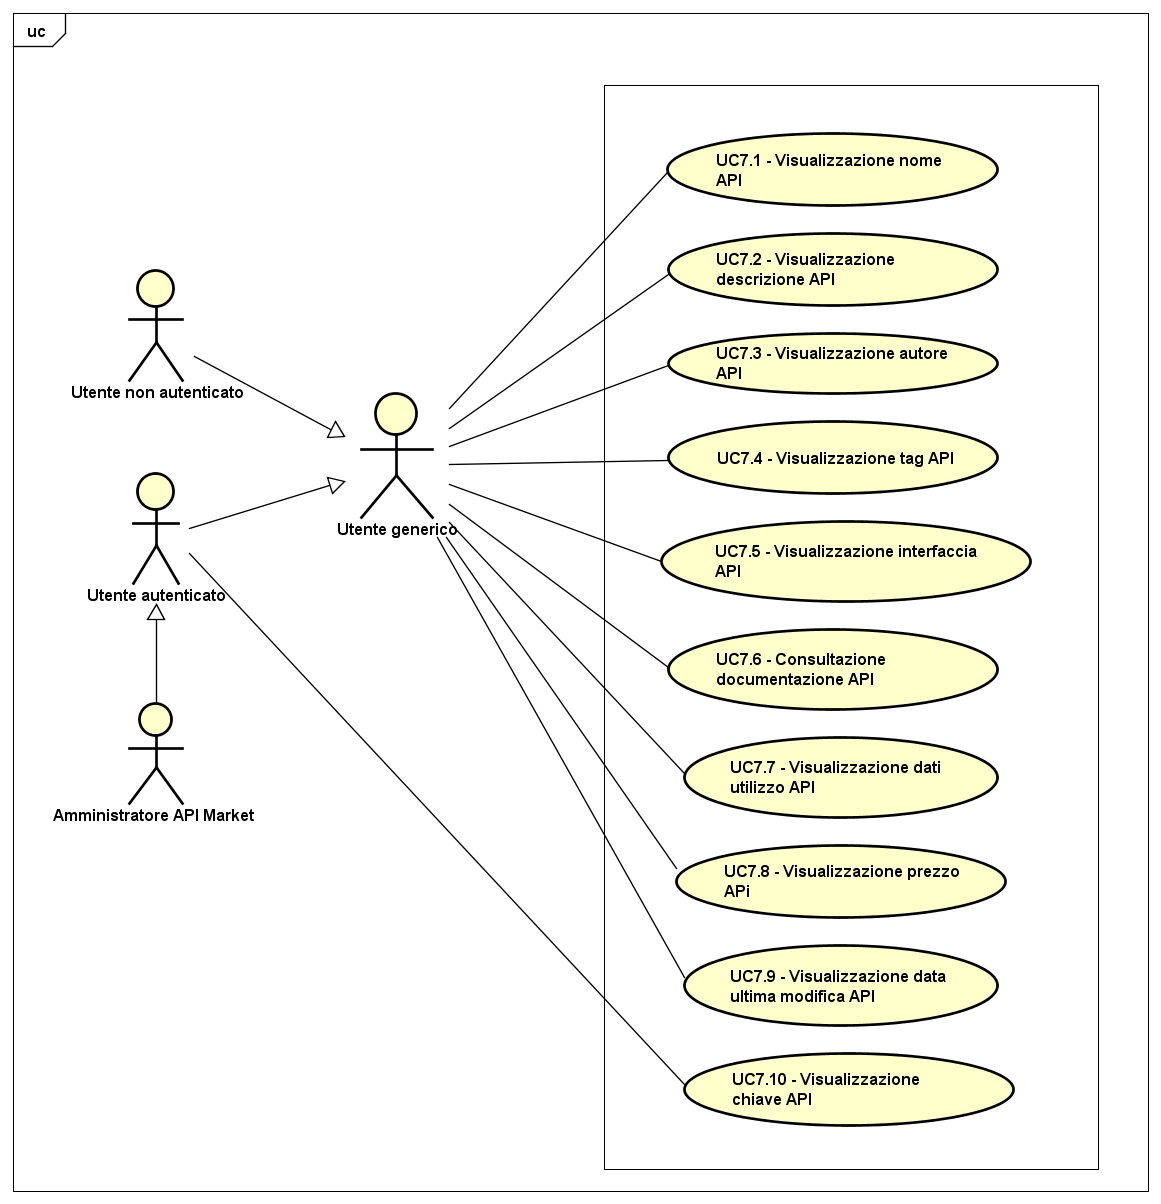
\includegraphics[scale=0.45]{UML/UC7.png}
	\caption{UC7: Visualizzazione API}
\end{figure}

\begin{longtable}{ l | p{11cm}}
	\hline
	\rowcolor{Gray}
	\multicolumn{2}{c}{UC7 - Visualizzazione API}\\
	\hline
	
	 \textbf{Attori} & Utente non autenticato, Utente autenticato  \\
	\textbf{Descrizione} & L'attore può visualizzare i dati relativi a un API che ha selezionato tramite la homepage o i risultati di una ricerca  \\
	\textbf{Pre-Condizioni} & L'attore ha selezionato un prodotto per la consultazione \\
	\textbf{Post-Condizioni} & L'attore visualizza la pagina relativa all'API selezionata\\
	\textbf{Scenario Principale} & 
	\begin{enumerate*}[label=(\arabic*.),itemjoin={\newline}]
		\item L'attore visualizza il nome dell'API (UC7.1)
		\item L'attore visualizza la descrizione dell'API (UC7.2)
		\item L'attore visualizza l'autore dell'API (UC7.3)
		\item L'attore visualizza i tag registrati relativi all'API (UC7.4)
		\item L'attore può visualizzare l'interfaccia dell'API (UC7.5)
		\item L'attore può consultare la documentazione fornita dall'utente (UC7.6)
		\item L'attore può visualizzare i dati di utilizzo dell'API  (UC7.7)
		\item L'attore visualizza il prezzo dell'API (UC7.8)
		\item L'attore può acquistare l'API visualizzata (UC9)
	\end{enumerate*}\\
	\textbf{Scenari Alternativi} & 
	\begin{enumerate*}[label=(\arabic*.),itemjoin={\newline}]
		\item L'attore possiede una licenza attiva per il prodotto, e può visualizzarne la chiave personale di utilizzo (UC7.9)
	\end{enumerate*}\\
\end{longtable}


\subsubsection{Caso d'uso UC7.1: Visualizzazione nome API}
\label{UC7_1}

\begin{minipage}{\linewidth}
	\begin{tabular}{ l | p{11cm}}
		\hline
		\rowcolor{Gray}
		\multicolumn{2}{c}{UC7.1 - Visualizza nome API} \\
		\hline
		\textbf{Attori} & Utente non autenticato, Utente autenticato \\
		\textbf{Descrizione} & L'attore visualizza il nome dell'API nella schermata relativa\\
		\textbf{Pre-Condizioni} & L'attore ha selezionato un API per poterla visualizzare\\
		\textbf{Post-Condizioni} & L'attore visualizza il nome dell'API selezionata \\
		\textbf{Scenario Principale} & 
		\begin{enumerate*}[label=(\arabic*.),itemjoin={\newline}]
			\item L'attore può visualizzare il nome dell'API selezionata
		\end{enumerate*}\\
	\end{tabular}
\end{minipage}

\subsubsection{Caso d'uso UC7.2: Visualizzazione descrizione API}
\label{UC7_2}

\begin{minipage}{\linewidth}
	\begin{tabular}{ l | p{11cm}}
		\hline
		\rowcolor{Gray}
		\multicolumn{2}{c}{UC7.2 - Visualizzazione descrizione API} \\
		\hline
		\textbf{Attori} & Utente non autenticato, Utente autenticato \\
		\textbf{Descrizione} & L'attore visualizza la descrizione dell'API nella schermata relativa\\
		\textbf{Pre-Condizioni} & L'attore ha selezionato un API per poterla visualizzare\\
		\textbf{Post-Condizioni} & L'attore visualizza la descrizione dell'API selezionata \\
		\textbf{Scenario Principale} & 
		\begin{enumerate*}[label=(\arabic*.),itemjoin={\newline}]
			\item L'attore può visualizzare la descrizione dell'API selezionata
		\end{enumerate*}\\
	\end{tabular}
\end{minipage}

\subsubsection{Caso d'uso UC7.3: Visualizzazione autore API}
\label{UC7_3}

\begin{minipage}{\linewidth}
	\begin{tabular}{ l | p{11cm}}
		\hline
		\rowcolor{Gray}
		\multicolumn{2}{c}{UC7.3 - Visualizzazione autore API} \\
		\hline
		\textbf{Attori} & Utente non autenticato, Utente autenticato \\
		\textbf{Descrizione} & L'attore visualizza il nome dell'autore dell'API nella schermata relativa\\
		\textbf{Pre-Condizioni} & L'attore ha selezionato un API per poterla visualizzare\\
		\textbf{Post-Condizioni} & L'attore visualizza il nome dell'autore per l'API selezionata \\
		\textbf{Scenario Principale} & 
		\begin{enumerate*}[label=(\arabic*.),itemjoin={\newline}]
			\item L'attore può visualizzare il nome dell'autore per l'API selezionata
		\end{enumerate*}\\
	\end{tabular}
\end{minipage}

\subsubsection{Caso d'uso UC7.4: Visualizzazione tag API}
\label{UC7_4}

\begin{minipage}{\linewidth}
	\begin{tabular}{ l | p{11cm}}
		\hline
		\rowcolor{Gray}
		\multicolumn{2}{c}{UC7.4 - Visualizzazione tag API} \\
		\hline
		\textbf{Attori} & Utente non autenticato, Utente autenticato \\
		\textbf{Descrizione} & L'attore visualizza i tag dell'API nella schermata relativa\\
		\textbf{Pre-Condizioni} & L'attore ha selezionato un API per poterla visualizzare\\
		\textbf{Post-Condizioni} & L'attore visualizza i tag per l'API selezionata \\
		\textbf{Scenario Principale} & 
		\begin{enumerate*}[label=(\arabic*.),itemjoin={\newline}]
			\item L'attore può visualizzare i tag assegnati all'API selezionata
		\end{enumerate*}\\
	\end{tabular}
\end{minipage}

\subsubsection{Caso d'uso UC7.5: Visualizzazione interfaccia API}
\label{UC7_5}

\begin{minipage}{\linewidth}
	\begin{tabular}{ l | p{11cm}}
		\hline
		\rowcolor{Gray}
		\multicolumn{2}{c}{UC7.5 - Visualizzazione interfaccia API} \\
		\hline
		\textbf{Attori} & Utente non autenticato, Utente autenticato \\
		\textbf{Descrizione} & L'attore visualizza l'interfaccia dell'API nella schermata relativa\\
		\textbf{Pre-Condizioni} & L'attore ha selezionato un API per poterla visualizzare\\
		\textbf{Post-Condizioni} & L'attore visualizza l'interfaccia dell'API selezionata \\
		\textbf{Scenario Principale} & 
		\begin{enumerate*}[label=(\arabic*.),itemjoin={\newline}]
			\item L'attore può visualizzare l'interfaccia dell'API selezionata
		\end{enumerate*}\\
	\end{tabular}
\end{minipage}

\subsubsection{Caso d'uso UC7.6: Visualizzazione documentazione API}
\label{UC7_6}

\begin{minipage}{\linewidth}
	\begin{tabular}{ l | p{11cm}}
		\hline
		\rowcolor{Gray}
		\multicolumn{2}{c}{UC7.6 - Visualizzazione documentazione API} \\
		\hline
		\textbf{Attori} & Utente non autenticato, Utente autenticato \\
		\textbf{Descrizione} & L'attore può visualizzare la documentazione dell'API\\
		\textbf{Pre-Condizioni} & L'attore ha selezionato un API per poterla visualizzare\\
		\textbf{Post-Condizioni} & L'attore visualizza la documentazione dell'API selezionata \\
		\textbf{Scenario Principale} & 
		\begin{enumerate*}[label=(\arabic*.),itemjoin={\newline}]
			\item L'attore può visualizzare la documentazione dell'API selezionata tramite un link esterno fornita dall'autore (UC7.6.1)
			\item L'attore può visualizzare la documentazione dell'API selezionata scaricando il file PDF fornito dall'autore (UC7.6.2)
		\end{enumerate*}\\
	\end{tabular}
\end{minipage}

\subsubsection{Caso d'uso UC7.6.1: Visualizzazione esterna documentazione}
\label{UC7_6_1}

\begin{minipage}{\linewidth}
	\begin{tabular}{ l | p{11cm}}
		\hline
		\rowcolor{Gray}
		\multicolumn{2}{c}{UC7.6.1 - Visualizzazione esterna documentazione} \\
		\hline
		\textbf{Attori} & Utente non autenticato, Utente autenticato, Pagina web esterna \\
		\textbf{Descrizione} & L'attore può visualizzare la documentazione dell'API tramite un link esterno fornito dall'autore\\
		\textbf{Pre-Condizioni} & L'attore visualizza un link relativo alla documentazione esterna\\
		\textbf{Post-Condizioni} & L'attore apre il link, e viene reindirizzato ad una pagina esterna fornita dall'autore dell'API \\
		\textbf{Scenario Principale} & 
		\begin{enumerate*}[label=(\arabic*.),itemjoin={\newline}]
			\item L'attore visita la pagina esterna per consultare la documentazione fornita dall'autore
		\end{enumerate*}\\
	\end{tabular}
\end{minipage}

\subsubsection{Caso d'uso UC7.6.2: Scarica documentazione PDF}
\label{UC7_6_2}

\begin{minipage}{\linewidth}
	\begin{tabular}{ l | p{11cm}}
		\hline
		\rowcolor{Gray}
		\multicolumn{2}{c}{UC7.6.2 - Scarica documentazione PDF} \\
		\hline
		\textbf{Attori} & Utente non autenticato, Utente autenticato \\
		\textbf{Descrizione} & L'attore può scaricare la documentazione dell'API in formato PDF\\
		\textbf{Pre-Condizioni} & L'attore visualizza un link relativo alla documentazione in PDF\\
		\textbf{Post-Condizioni} & L'attore seleziona il link di download e scarica la documentazione in formato PDF \\
		\textbf{Scenario Principale} & 
		\begin{enumerate*}[label=(\arabic*.),itemjoin={\newline}]
			\item L'attore può scaricare la documentazione fornita dall'autore dell'API in formato PDF
		\end{enumerate*}\\
	\end{tabular}
\end{minipage}

\subsubsection{Caso d'uso UC7.7: Visualizzazione dati utilizzo API}
\label{UC7_7}

\begin{minipage}{\linewidth}
	\begin{tabular}{ l | p{11cm}}
		\hline
		\rowcolor{Gray}
		\multicolumn{2}{c}{UC7.7 - Visualizzazione dati utilizzo API} \\
		\hline
		\textbf{Attori} & Utente non autenticato, Utente autenticato \\
		\textbf{Descrizione} & L'attore visualizza i dati di utilizzo dell'API nella schermata relativa\\
		\textbf{Pre-Condizioni} & L'attore ha selezionato un API per poterla visualizzare\\
		\textbf{Post-Condizioni} & L'attore visualizza i dati di utilizzo per l'API selezionata \\
		\textbf{Scenario Principale} & 
		\begin{enumerate*}[label=(\arabic*.),itemjoin={\newline}]
			\item L'attore può visualizzare il numero di licenze attive (UC7.7.1)
			\item L'attore può visualizzare il numero di chiamate giornaliere effettuate (UC7.7.2)
			\item L'attore può visualizzare il tempo medio di utilizzo (UC7.7.3)
			\item L'attore può visualizzare il quantitativo di dati scambiati (UC7.7.4)
		\end{enumerate*}\\
	\end{tabular}
\end{minipage}

\subsubsection{Caso d'uso UC7.7.1: Visualizzazione licenze attive}
\label{UC7_7.1}

\begin{minipage}{\linewidth}
	\begin{tabular}{ l | p{11cm}}
		\hline
		\rowcolor{Gray}
		\multicolumn{2}{c}{UC7.7.1 - Visualizzazione licenze attive} \\
		\hline
		\textbf{Attori} & Utente non autenticato, Utente autenticato \\
		\textbf{Descrizione} & L'attore visualizza il numero di licenze attive \\
		\textbf{Pre-Condizioni} & L'attore si trova nella schermata relativa ad una singola API\\
		\textbf{Post-Condizioni} & L'attore visualizza il numero di licenze attive per l'API selezionata \\
		\textbf{Scenario Principale} & 
		\begin{enumerate*}[label=(\arabic*.),itemjoin={\newline}]
			\item L'attore può visualizzare il numero di licenze attive per l'API selezionata
		\end{enumerate*}\\
	\end{tabular}
\end{minipage}

\subsubsection{Caso d'uso UC7.7.2: Visualizzazione chiamate giornaliere}
\label{UC7_7.2}

\begin{minipage}{\linewidth}
	\begin{tabular}{ l | p{11cm}}
		\hline
		\rowcolor{Gray}
		\multicolumn{2}{c}{UC7.7.2 - Visualizzazione chiamate giornaliere} \\
		\hline
		\textbf{Attori} & Utente non autenticato, Utente autenticato \\
		\textbf{Descrizione} & L'attore visualizza il numero di chiamate giornaliere \\
		\textbf{Pre-Condizioni} & L'attore si trova nella schermata relativa ad una singola API\\
		\textbf{Post-Condizioni} & L'attore visualizza il numero di chiamate giornaliere per l'API selezionata \\
		\textbf{Scenario Principale} & 
		\begin{enumerate*}[label=(\arabic*.),itemjoin={\newline}]
			\item L'attore può visualizzare il numero di chiamate giornaliere per l'API selezionata
		\end{enumerate*}\\
	\end{tabular}
\end{minipage}

\subsubsection{Caso d'uso UC7.7.3: Visualizzazione tempo medio di utilizzo}
\label{UC7_7.3}

\begin{minipage}{\linewidth}
	\begin{tabular}{ l | p{11cm}}
		\hline
		\rowcolor{Gray}
		\multicolumn{2}{c}{UC7.7.3 - Visualizzazione tempo medio di utilizzo} \\
		\hline
		\textbf{Attori} & Utente non autenticato, Utente autenticato \\
		\textbf{Descrizione} & L'attore visualizza il tempo medio di utilizzo \\
		\textbf{Pre-Condizioni} & L'attore si trova nella schermata relativa ad una singola API\\
		\textbf{Post-Condizioni} & L'attore visualizza il tempo medio di utilizzo per l'API selezionata \\
		\textbf{Scenario Principale} & 
		\begin{enumerate*}[label=(\arabic*.),itemjoin={\newline}]
			\item L'attore può visualizzare il tempo medio di utilizzo per l'API selezionata
		\end{enumerate*}\\
	\end{tabular}
\end{minipage}

\subsubsection{Caso d'uso UC7.7.4: Visualizzazione dati scambiati}
\label{UC7_7.4}

\begin{minipage}{\linewidth}
	\begin{tabular}{ l | p{11cm}}
		\hline
		\rowcolor{Gray}
		\multicolumn{2}{c}{UC7.7.4 - Visualizzazione dati scambiati} \\
		\hline
		\textbf{Attori} & Utente non autenticato, Utente autenticato \\
		\textbf{Descrizione} & L'attore visualizza il quantitativo di dati scambiati tra l'utilizzatore e il microservizio \\
		\textbf{Pre-Condizioni} & L'attore si trova nella schermata relativa ad una singola API\\
		\textbf{Post-Condizioni} & L'attore visualizza il quantitativo di dati scambiati per l'API selezionata \\
		\textbf{Scenario Principale} & 
		\begin{enumerate*}[label=(\arabic*.),itemjoin={\newline}]
			\item L'attore può visualizzare il quantitativo di dati scambiati per l'API selezionata
		\end{enumerate*}\\
	\end{tabular}
\end{minipage}

\subsubsection{Caso d'uso UC7.8: Visualizzazione chiave API}
\label{UC7_8}

\begin{minipage}{\linewidth}
	\begin{tabular}{ l | p{11cm}}
		\hline
		\rowcolor{Gray}
		\multicolumn{2}{c}{UC7.8 - Visualizzazione chiave API} \\
		\hline
		\textbf{Attori} & Utente autenticato \\
		\textbf{Descrizione} & L'attore visualizza la propria chiave di utilizzo per l'API\\
		\textbf{Pre-Condizioni} & L'attore possiede una licenza attualmente attiva per l'API in questione\\
		\textbf{Post-Condizioni} & L'attore visualizza la propria chiave API \\
		\textbf{Scenario Principale} & 
		\begin{enumerate*}[label=(\arabic*.),itemjoin={\newline}]
			\item L'attore può visualizzare la propria chiave API personale
		\end{enumerate*}\\
	\end{tabular}
\end{minipage}

\subsubsection{Caso d'uso UC7.9: Visualizzazione prezzo API}
\label{UC7_9}

\begin{minipage}{\linewidth}
	\begin{tabular}{ l | p{11cm}}
		\hline
		\rowcolor{Gray}
		\multicolumn{2}{c}{UC7.9 - Visualizzazione prezzo API} \\
		\hline
		\textbf{Attori} & Utente non autenticato, Utente autenticato \\
		\textbf{Descrizione} & L'attore visualizza il prezzo dell'API selezionata\\
		\textbf{Pre-Condizioni} & L'attore ha selezionato un API per poterla visualizzare\\
		\textbf{Post-Condizioni} & L'attore visualizza il prezzo per l'API selezionata \\
		\textbf{Scenario Principale} & 
		\begin{enumerate*}[label=(\arabic*.),itemjoin={\newline}]
			\item L'attore può visualizzare il prezzo per l'API nella pagina corrente
		\end{enumerate*}\\
	\end{tabular}
\end{minipage}
\newpage
\subsection{Caso d'uso UC8 - Visualizzazione API acquistate}
\label{UC8}
\begin{figure}[ht]
	\centering
	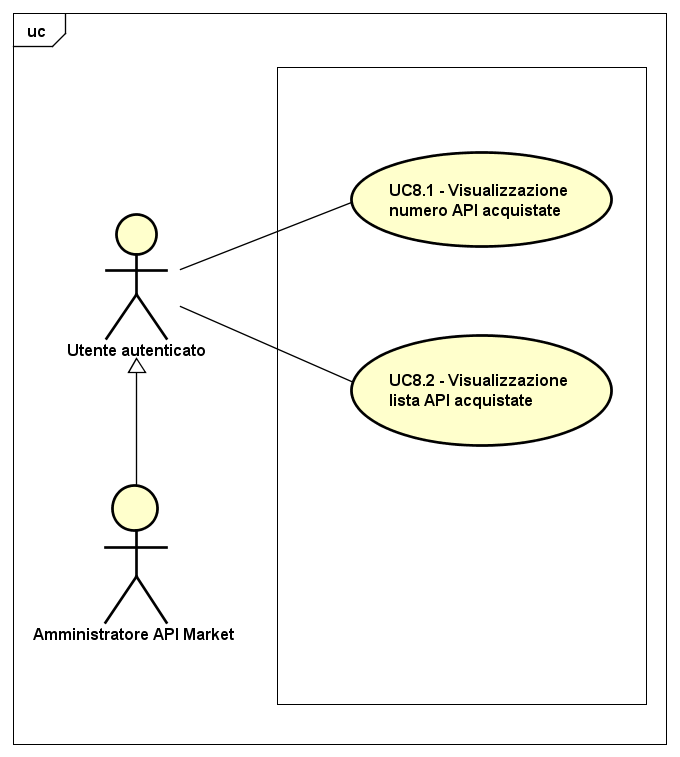
\includegraphics[scale=0.45]{UML/UC8.png}
	\caption{UC8: Visualizzazione API acquistate}
\end{figure}

\begin{longtable}{ l | p{11cm}}
	\hline
	\rowcolor{Gray}
	\multicolumn{2}{c}{UC8 - Visualizzazione API acquistate}\\
	\hline
	 \textbf{Attori} & Utente autenticato, Amministratore API Market \\
	\textbf{Descrizione} & L'attore visualizza le API da lui acquistate \\
	\textbf{Pre-Condizioni} & L'attore si trova nella schermata relativa alle API da lui acquistate \\
	\textbf{Post-Condizioni} & L'attore ha visualizzato le API da lui acquistate \\
	\textbf{Scenario Principale} & 
	\begin{enumerate*}[label=(\arabic*.),itemjoin={\newline}]
		\item L'attore può visualizzare il numero delle API acquistate e attive (UC8.1)
		\item L'attore può visualizzare la lista delle API acquistate e attive (UC8.2)
	\end{enumerate*}\\
	\textbf{Scenari Alternativi} & 
	\begin{enumerate*}[label=(\arabic*.),itemjoin={\newline}]
		\item L'attore può visualizzare i dati relativi ad una singola API (UC7)
	\end{enumerate*}\\
\end{longtable}

\subsubsection{Caso d'uso UC8.1: Visualizzazione numero API acquistate}
\label{UC8_1}

\begin{minipage}{\linewidth}
	\begin{tabular}{ l | p{11cm}}
		\hline
		\rowcolor{Gray}
		\multicolumn{2}{c}{UC8.1 - Visualizzazione numero API acquistate} \\
		\hline
		\textbf{Attori} & Utente autenticato, Amministratore API Market \\
		\textbf{Descrizione} & L'attore visualizza il numero di API da lui acquistate \\
		\textbf{Pre-Condizioni} & L'attore si trova nella schermata relativa alle API da lui acquistate \\
		\textbf{Post-Condizioni} & L'attore ha visualizzato il numero delle API da lui acquistate \\
		\textbf{Scenario Principale} & 
		\begin{enumerate*}[label=(\arabic*.),itemjoin={\newline}]
			\item L'attore può visualizzare il numero di API acquistate
		\end{enumerate*}\\
	\end{tabular}
\end{minipage}

\newpage
\subsubsection{Caso d'uso UC8.2: Visualizzazione lista API acquistate}
\label{UC8_2}
\begin{figure}[ht]
	\centering
	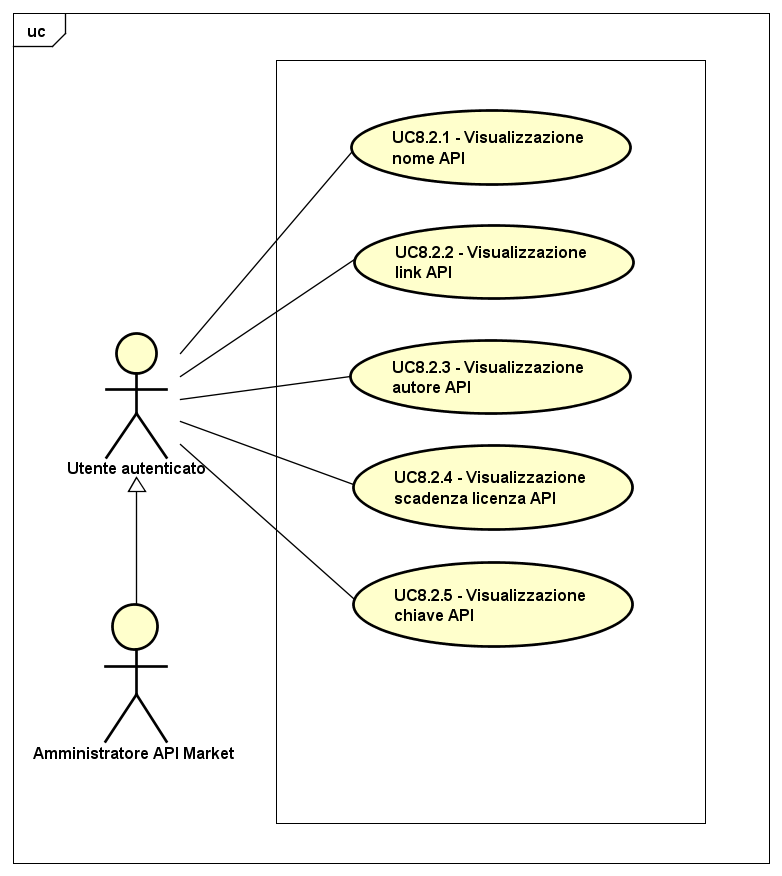
\includegraphics[scale=0.45]{UML/UC8_2.png}
	\caption{UC8.2: Visualizzazione lista API acquistate}
\end{figure}

\begin{minipage}{\linewidth}
	\begin{tabular}{ l | p{11cm}}
		\hline
		\rowcolor{Gray}
		\multicolumn{2}{c}{UC8.2 - Visualizzazione lista API acquistate} \\
		\hline
		\textbf{Attori} & Utente autenticato, Amministratore API Market \\
		\textbf{Descrizione} & L'attore visualizza la lista delle API da lui acquistate \\
		\textbf{Pre-Condizioni} & L'attore si trova nella schermata relativa alle API da lui acquistate \\
		\textbf{Post-Condizioni} & L'attore ha visualizzato la lista delle API da lui acquistate \\
		\textbf{Scenario Principale} & 
		\begin{enumerate*}[label=(\arabic*.),itemjoin={\newline}]
			\item L'attore può visualizzare il nome dell'API (UC8.2.1)
			\item L'attore può visualizzare il link alla pagina di visualizzazione API (UC8.2.2)
			\item L'attore può visualizzare il nome dell'autore dell'API (UC8.2.3)
			\item L'attore può visualizzare il parametro di scadenza, in base al contratto,  della propria licenza per l'API (UC8.2.4)
			\item L'attore può visualizzare la propria chiave per l'API (UC8.2.5)
		\end{enumerate*}\\
	\end{tabular}
\end{minipage}

\paragraph{Caso d'uso UC8.2.1: Visualizzazione nome API}
\label{UC8_2_1}

\begin{minipage}{\linewidth}
	\begin{tabular}{ l | p{11cm}}
		\hline
		\rowcolor{Gray}
		\multicolumn{2}{c}{UC8.2.1 - Visualizzazione nome API} \\
		\hline
		\textbf{Attori} & Utente autenticato, Amministratore API Market \\
		\textbf{Descrizione} & L'attore visualizza nella lista il nome dell'API \\
		\textbf{Pre-Condizioni} & L'attore si trova nella schermata relativa alle API da lui acquistate \\
		\textbf{Post-Condizioni} & L'attore ha visualizzato nella lista il nome dell'API \\
		\textbf{Scenario Principale} & 
		\begin{enumerate*}[label=(\arabic*.),itemjoin={\newline}]
			\item L'attore può visualizzare nella lista il nome dell'API
		\end{enumerate*}\\
	\end{tabular}
\end{minipage}

\paragraph{Caso d'uso UC8.2.2: Visualizzazione link API}
\label{UC8_2_2}

\begin{minipage}{\linewidth}
	\begin{tabular}{ l | p{11cm}}
		\hline
		\rowcolor{Gray}
		\multicolumn{2}{c}{UC8.2.2 - Visualizzazione link API} \\
		\hline
		\textbf{Attori} & Utente autenticato, Amministratore API Market \\
		\textbf{Descrizione} & L'attore visualizza nella lista il link alla visualizzazione dell'API \\
		\textbf{Pre-Condizioni} & L'attore si trova nella schermata di visualizzazione dell'API acquistate \\
		\textbf{Post-Condizioni} & L'attore ha visualizzato nella lista il link alla visualizzazione dell'API \\
		\textbf{Scenario Principale} & 
		\begin{enumerate*}[label=(\arabic*.),itemjoin={\newline}]
			\item L'attore può visualizzare nella lista il link alla visualizzazione dell'API
		\end{enumerate*}\\
	\end{tabular}
\end{minipage}

\paragraph{Caso d'uso UC8.2.4: Visualizzazione scadenza licenza}
\label{UC8_2_4}

\begin{minipage}{\linewidth}
	\begin{tabular}{ l | p{11cm}}
		\hline
		\rowcolor{Gray}
		\multicolumn{2}{c}{UC8.2.3 - Visualizzazione scadenza licenza} \\
		\hline
		\textbf{Attori} & Utente autenticato, Amministratore API Market \\
		\textbf{Descrizione} & L'attore visualizza nella lista la data di scadenza della propria licenza per l'API \\
		\textbf{Pre-Condizioni} & L'attore si trova nella schermata relativa alle API da lui acquistate \\
		\textbf{Post-Condizioni} & L'attore ha visualizzato nella lista il parametro di scadenza dell'API \\
		\textbf{Scenario Principale} & 
		\begin{enumerate*}[label=(\arabic*.),itemjoin={\newline}]
			\item L'attore può visualizzare nella lista il parametro di scadenza della propria licenza per l'API
		\end{enumerate*}\\
	\end{tabular}
\end{minipage}

\paragraph{Caso d'uso UC8.2.5: Visualizzazione chiave API}
\label{UC8_2_5}

\begin{minipage}{\linewidth}
	\begin{tabular}{ l | p{11cm}}
		\hline
		\rowcolor{Gray}
		\multicolumn{2}{c}{UC8.2.5 - Visualizzazione chiave API} \\
		\hline
		\textbf{Attori} & Utente autenticato, Amministratore API Market \\
		\textbf{Descrizione} & L'attore visualizza nella lista la propria chiave di utilizzo per l'API \\
		\textbf{Pre-Condizioni} & L'attore si trova nella schermata relativa alle API da lui acquistate \\
		\textbf{Post-Condizioni} & L'attore ha visualizzato nella lista la propria chiave di utilizzo per l'API \\
		\textbf{Scenario Principale} & 
		\begin{enumerate*}[label=(\arabic*.),itemjoin={\newline}]
			\item L'attore può visualizzare nella lista la propria chiave di utilizzo per l'API
		\end{enumerate*}\\
	\end{tabular}
\end{minipage}

\paragraph{Caso d'uso UC8.2.6: Avvertimento eliminazione API}
\label{UC8_2_6}

\begin{minipage}{\linewidth}
	\begin{tabular}{ l | p{11cm}}
		\hline
		\rowcolor{Gray}
		\multicolumn{2}{c}{UC8.2.6 - Avvertimento eliminazione API} \\
		\hline
		\textbf{Attori} & Utente autenticato, Amministratore API Market \\
		\textbf{Descrizione} & L'attore visualizza nella lista se l'API \\
		\textbf{Pre-Condizioni} & L'attore si trova nella schermata relativa alle API da lui acquistate \\
		\textbf{Post-Condizioni} & L'attore ha visualizzato nella lista la propria chiave di utilizzo per l'API \\
		\textbf{Scenario Principale} & 
		\begin{enumerate*}[label=(\arabic*.),itemjoin={\newline}]
			\item L'attore può visualizzare nella lista la propria chiave di utilizzo per l'API
		\end{enumerate*}\\
	\end{tabular}
\end{minipage}
\newpage
\subsection{Caso d'uso UC9 - Acquisto API}
\label{UC9}
\begin{figure}[ht]
	\centering
	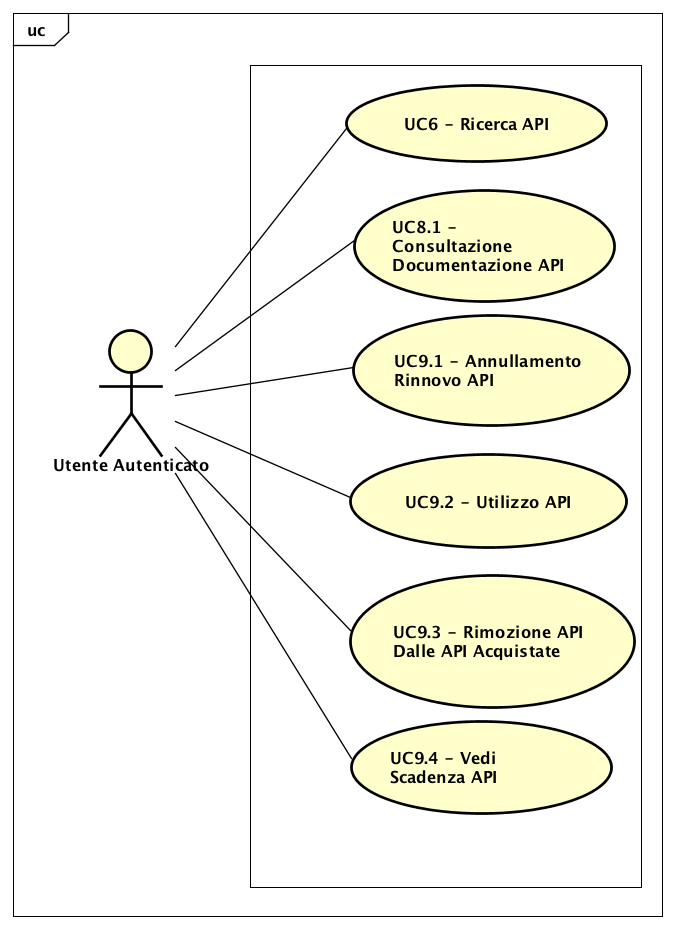
\includegraphics[scale=0.45]{UML/UC9.png}
	\caption{UC9: Acquisto API}
\end{figure}

\begin{longtable}{ l | p{11cm}}
	\hline
	\rowcolor{Gray}
	\multicolumn{2}{c}{UC9 - Acquisto API}\\
	\hline
	\textbf{Attori} & Utente autenticato, Amministratore API Market \\
	\textbf{Descrizione} & L'attore può effettuare l'acquisto dell'API selezionata tramite i crediti da lui posseduti \\
	\textbf{Pre-Condizioni} & L'attore ha selezionato una API e si trova nella relativa schermata di acquisto \\
	\textbf{Post-Condizioni} & L'attore ha acquistato l'API selezionata \\
	\textbf{Scenario Principale} & 
	\begin{enumerate*}[label=(\arabic*.),itemjoin={\newline}]
		\item L'attore può visualizzare il nome dell'API (UC7.1)
		\item L'attore può visualizzare l'autore dell'API (UC7.3)
		\item L'attore può scegliere la licenza API desiderata (UC9.1)
		\item L'attore può visualizzare il prezzo dell'API selezionata (UC7.8)
		\item L'attore può visualizzare il saldo disponibile nel suo conto virtuale (UC12.2.1)
		\item L'attore può ricaricare il proprio conto virtuale (UC12.2.2)
		\item L'attore può visualizzare il saldo preventivato in seguito all'acquisto della licenza selezionata (UC9.2)
		\item L'attore può confermare l'acquisto (UC9.3), venendo reindirizzato ad una schermata di riepilogo (UC9.4)
	\end{enumerate*}\\
	\textbf{Scenari Alternativi} & 
	\begin{enumerate*}[label=(\arabic*.),itemjoin={\newline}]
		\item L'attore può visualizzare un messaggio di errore e la transazione non avviene (UC9.5)
	\end{enumerate*}\\
\end{longtable}

\newpage
\subsubsection{Caso d'uso UC9.1: Scelta licenza API}
\label{UC9_1}
\begin{figure}[ht]
	\centering
	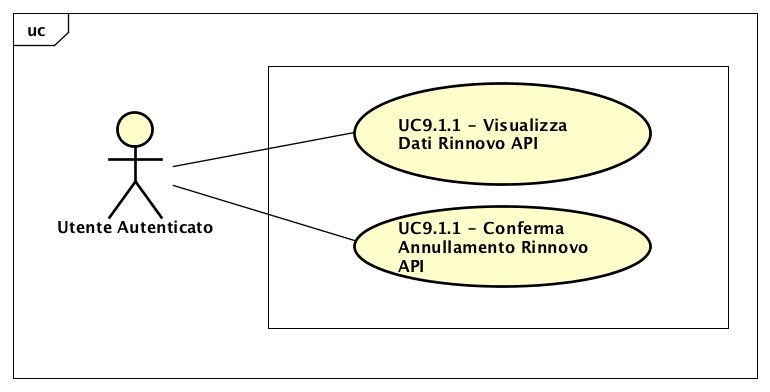
\includegraphics[scale=0.45]{UML/UC9_1.png}
	\caption{UC9.1: Scelta licenza API}
\end{figure}

\begin{minipage}{\linewidth}
	\begin{tabular}{ l | p{11cm}}
		\hline
		\rowcolor{Gray}
		\multicolumn{2}{c}{UC9.1 - Visualizzazione menù licenza} \\
		\hline
		\textbf{Attori} & Utente autenticato, Amministratore API Market \\
		\textbf{Descrizione} & L'attore sceglie tra le licenze quella desiderata, oppure lascia inalterata la scelta di default \\
		\textbf{Pre-Condizioni} & L'attore ha selezionato una API e si trova nella relativa schermata di acquisto \\
		\textbf{Post-Condizioni} & L'attore ha selezionato la licenza desiderata, oppure ha lasciato inalterata la scelta di default \\
		\textbf{Scenario Principale} & 
		\begin{enumerate*}[label=(\arabic*.),itemjoin={\newline}]
			\item L'attore può selezionare la licenza per numero di chiamate, impostata di default (UC9.1.1)
			\item L'attore può selezionare la licenza per tempo di utilizzo (UC9.1.2)
			\item L'attore può selezionare la licenza per traffico (UC9.1.3)
		\end{enumerate*}\\
	\end{tabular}
\end{minipage}

\paragraph{Caso d'uso UC9.1.1: Scelta licenza per numero di chiamate}
\label{UC9_1_1}

\begin{minipage}{\linewidth}
	\begin{tabular}{ l | p{11cm}}
		\hline
		\rowcolor{Gray}
		\multicolumn{2}{c}{UC9.1.1 - Scelta licenza per numero di chiamate} \\
		\hline
		\textbf{Attori} & Utente autenticato, Amministratore API Market \\
		\textbf{Descrizione} & L'attore sceglie la licenza API per numero di chiamate \\
		\textbf{Pre-Condizioni} & L'attore visualizza il menù per la scelta della licenza API  \\
		\textbf{Post-Condizioni} & L'attore ha scelto la licenza API per numero di chiamate \\
		\textbf{Scenario Principale} & 
		\begin{enumerate*}[label=(\arabic*.),itemjoin={\newline}]
			\item L'attore può scegliere la licenza API per numero di chiamate
		\end{enumerate*}\\
	\end{tabular}
\end{minipage}

\paragraph{Caso d'uso UC9.1.2: Scelta licenza per tempo di utilizzo}
\label{UC9_1_2}

\begin{minipage}{\linewidth}
	\begin{tabular}{ l | p{11cm}}
		\hline
		\rowcolor{Gray}
		\multicolumn{2}{c}{UC9.1.2 - Scelta licenza per tempo di utilizzo} \\
		\hline
		\textbf{Attori} & Utente autenticato, Amministratore API Market \\
		\textbf{Descrizione} & L'attore sceglie la licenza API per tempo di utilizzo \\
		\textbf{Pre-Condizioni} & L'attore visualizza il menù per la scelta della licenza API  \\
		\textbf{Post-Condizioni} & L'attore ha scelto la licenza API per tempo di utilizzo \\
		\textbf{Scenario Principale} & 
		\begin{enumerate*}[label=(\arabic*.),itemjoin={\newline}]
			\item L'attore può scegliere la licenza API per tempo di utilizzo
		\end{enumerate*}\\
	\end{tabular}
\end{minipage}

\paragraph{Caso d'uso UC9.1.3: Scelta licenza per traffico}
\label{UC9_1_3}

\begin{minipage}{\linewidth}
	\begin{tabular}{ l | p{11cm}}
		\hline
		\rowcolor{Gray}
		\multicolumn{2}{c}{UC9.1.3 - Scelta licenza per traffico} \\
		\hline
		\textbf{Attori} & Utente autenticato, Amministratore API Market \\
		\textbf{Descrizione} & L'attore sceglie la licenza API per traffico \\
		\textbf{Pre-Condizioni} & L'attore visualizza il menù per la scelta della licenza API  \\
		\textbf{Post-Condizioni} & L'attore ha scelto la licenza API per traffico \\
		\textbf{Scenario Principale} & 
		\begin{enumerate*}[label=(\arabic*.),itemjoin={\newline}]
			\item L'attore può scegliere la licenza API per traffico
		\end{enumerate*}\\
	\end{tabular}
\end{minipage}

\subsubsection{Caso d'uso UC9.2: Visualizzazione previsione saldo finale}
\label{UC9_2}

\begin{minipage}{\linewidth}
	\begin{tabular}{ l | p{11cm}}
		\hline
		\rowcolor{Gray}
		\multicolumn{2}{c}{UC9.2 - Visualizzazione previsione saldo finale} \\
		\hline
		\textbf{Attori} & Utente autenticato, Amministratore API Market \\
		\textbf{Descrizione} & L'attore visualizza una previsione del proprio saldo crediti in seguito all'acquisto\\
		\textbf{Pre-Condizioni} & L'attore ha selezionato una API e si trova nella relativa schermata di acquisto \\
		\textbf{Post-Condizioni} & L'attore ha visualizzato una previsione del proprio saldo in seguito all'acquisto \\
		\textbf{Scenario Principale} & 
		\begin{enumerate*}[label=(\arabic*.),itemjoin={\newline}]
			\item L'attore può visualizzare una previsione del proprio saldo finale qualora acquistasse l'API con la licenza scelta in UC9.1
		\end{enumerate*}\\
	\end{tabular}
\end{minipage}

\subsubsection{Caso d'uso UC9.3: Conferma acquisto API}
\label{UC9_3}

\begin{minipage}{\linewidth}
	\begin{tabular}{ l | p{11cm}}
		\hline
		\rowcolor{Gray}
		\multicolumn{2}{c}{UC9.3 - Conferma acquisto API} \\
		\hline
		\textbf{Attori} & Utente autenticato, Amministratore API Market \\
		\textbf{Descrizione} & L'attore può confermare l'acquisto dell'API, portando a termine la transazione, ricevendo un'email di riepilogo e visualizzando una schermata di riepilogo dell'acquisto appena realizzato \\
		\textbf{Pre-Condizioni} & L'attore ha selezionato una API e si trova nella relativa schermata di acquisto \\
		\textbf{Post-Condizioni} & L'attore ha confermato l'acquisto dell'API \\
		\textbf{Scenario Principale} & 
		\begin{enumerate*}[label=(\arabic*.),itemjoin={\newline}]
			\item L'attore può confermare l'acquisto dell'API, portando a termine la transazione, ricevendo un'email di riepilogo e visualizzando una schermata di riepilogo dell'acquisto appena realizzato (UC9.4)
		\end{enumerate*}\\
	\end{tabular}
\end{minipage}

\subsubsection{Caso d'uso UC9.4: Riepilogo acquisto API}
\label{UC9_4}

\begin{minipage}{\linewidth}
	\begin{tabular}{ l | p{11cm}}
		\hline
		\rowcolor{Gray}
		\multicolumn{2}{c}{UC9.4 - Riepilogo acquisto API} \\
		\hline
		\textbf{Attori} & Utente autenticato, Amministratore API Market \\
		\textbf{Descrizione} & L'attore conferma l'acquisto dell'API, portando a termine la transazione e visualizzando un messaggio di ringraziamento \\
		\textbf{Pre-Condizioni} & L'attore ha confermato l'acquisto per l'API \\
		\textbf{Post-Condizioni} & L'attore ha visualizzato il riepilogo dell'acquisto appena realizzato \\
		\textbf{Scenario Principale} & 
		\begin{enumerate*}[label=(\arabic*.),itemjoin={\newline}]
			\item L'attore può visualizzare un messaggio di ringraziamento (UC9.4.1)
			\item L'attore può visualizzare il nome dell'API appena acquistata (UC7.1)
			\item L'attore può visualizzare la chiave dell'API appena acquistata (UC7.9)
		\end{enumerate*}\\
	\end{tabular}
\end{minipage}

\paragraph{Caso d'uso UC9.5: Errore acquisto API}
\label{UC9_5}

\begin{minipage}{\linewidth}
	\begin{tabular}{ l | p{11cm}}
		\hline
		\rowcolor{Gray}
		\multicolumn{2}{c}{UC9.5 - Errore acquisto API} \\
		\hline
		\textbf{Attori} & Utente autenticato, Amministratore API Market \\
		\textbf{Descrizione} & L'attore visualizza un messaggio di errore e la transazione non avviene \\
		\textbf{Pre-Condizioni} & L'attore ha confermato l'acquisto per una API ma si è verificato un errore \\
		\textbf{Post-Condizioni} & L'attore ha visualizzato un errore relativo all'acquisto, con opportuna descrizione \\
		\textbf{Scenario Principale} & 
		\begin{enumerate*}[label=(\arabic*.),itemjoin={\newline}]
			\item L'attore può visualizzare un messaggio di errore e la transazione non avviene (E.g: L'API è in fase di cancellazione)
		\end{enumerate*}\\
	\end{tabular}
\end{minipage}
\newpage
\subsection{Caso d'uso UC10 - Visualizzazione API registrate}
\label{UC10}
\begin{figure}[ht]
	\centering
	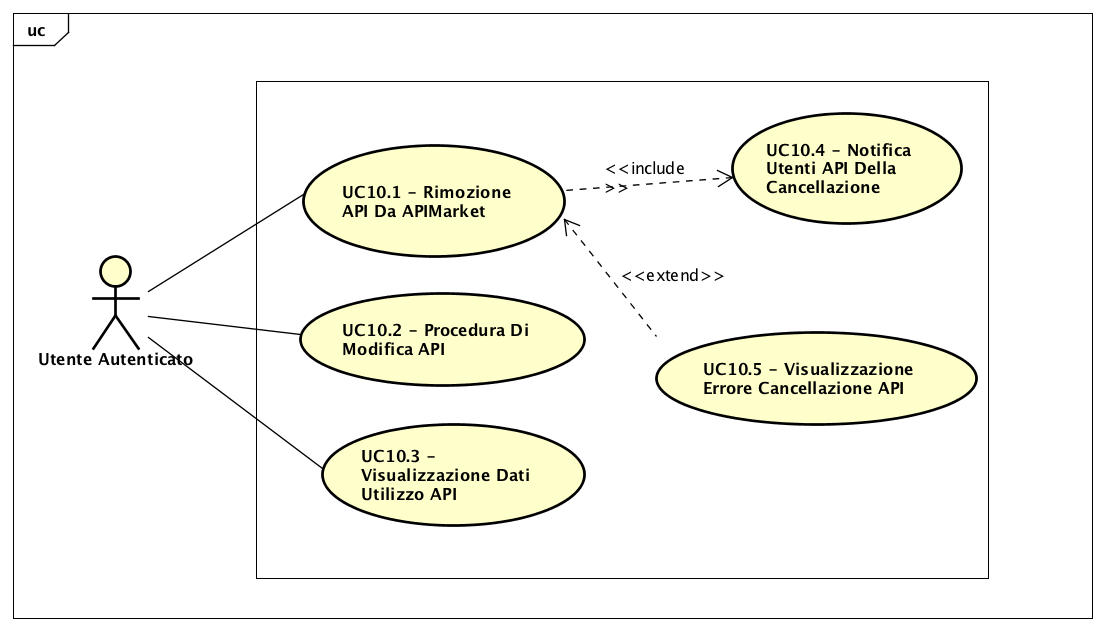
\includegraphics[scale=0.45]{UML/UC10.png}
	\caption{UC10: Visualizzazione API registrate}
\end{figure}

\begin{longtable}{ l | p{11cm}}
	\hline
	\rowcolor{Gray}
	\multicolumn{2}{c}{UC10 - Visualizzazione API registrate}\\
	\hline
	\textbf{Attori} & Utente autenticato, Amministratore API Market \\
	\textbf{Descrizione} & L'attore visualizza le API da lui registrate \\
	\textbf{Pre-Condizioni} & L'attore si trova nella schermata relativa alle API da lui registrate  \\
	\textbf{Post-Condizioni} & L'attore ha visualizzato le API da lui registrate \\
	\textbf{Scenario Principale} & 
	\begin{enumerate*}[label=(\arabic*.),itemjoin={\newline}]
		\item L'attore può visualizzare il numero delle API registrate (UC10.1)
		\item L'attore può visualizzare la lista delle API registrate (UC10.2)
	\end{enumerate*}\\
	\textbf{Scenari Alternativi} & 
	\begin{enumerate*}[label=(\arabic*.),itemjoin={\newline}]
		\item L'attore può visualizzare i dati relativi ad una singola API (UC7)
	\end{enumerate*}\\
\end{longtable}

\subsubsection{Caso d'uso UC10.1: Visualizzazione numero API registrate}
\label{UC10_1}

\begin{minipage}{\linewidth}
	\begin{tabular}{ l | p{11cm}}
		\hline
		\rowcolor{Gray}
		\multicolumn{2}{c}{UC10.1 - Visualizzazione numero API registrate} \\
		\hline
		\textbf{Attori} & Utente autenticato, Amministratore API Market \\
		\textbf{Descrizione} & L'attore visualizza il numero di API da lui registrate \\
		\textbf{Pre-Condizioni} & L'attore si trova nella schermata relativa alle API da lui registrate \\
		\textbf{Post-Condizioni} & L'attore ha visualizzato il numero delle API da lui registrate \\
		\textbf{Scenario Principale} & 
		\begin{enumerate*}[label=(\arabic*.),itemjoin={\newline}]
			\item L'attore può visualizzare il numero di API da lui registrate
		\end{enumerate*}\\
	\end{tabular}
\end{minipage}

\newpage
\subsubsection{Caso d'uso UC10.2: Visualizzazione lista API registrate}
\label{UC10_2}
\begin{figure}[ht]
	\centering
	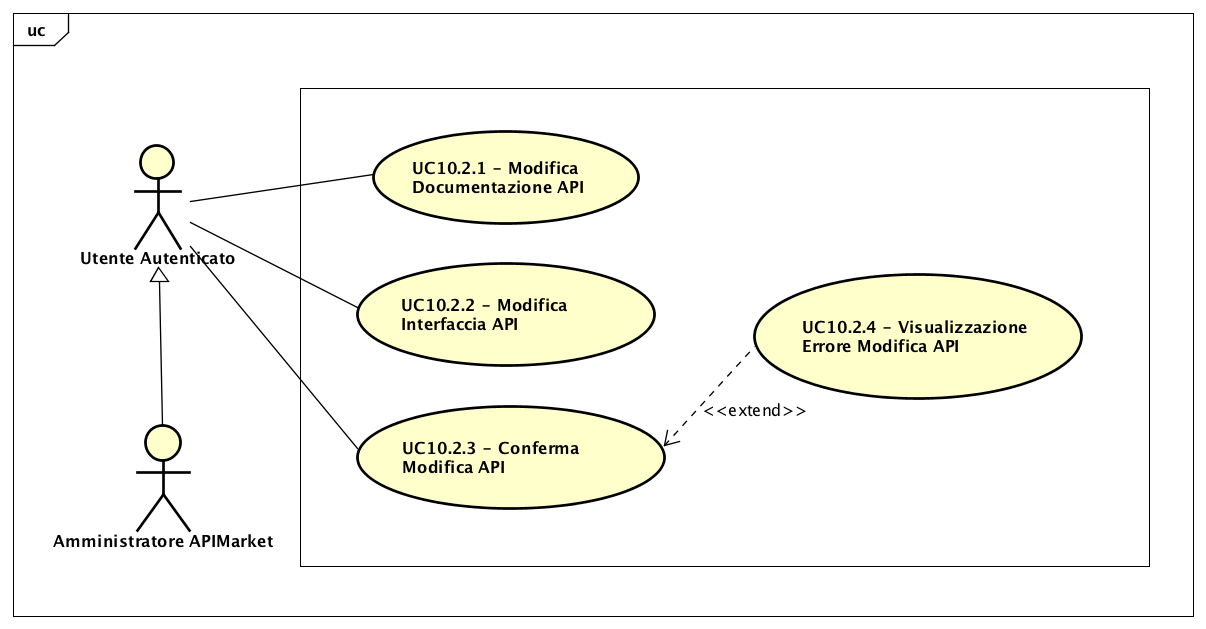
\includegraphics[scale=0.45]{UML/UC10_2.png}
	\caption{UC10.2: Visualizzazione lista API registrate}
\end{figure}

\begin{minipage}{\linewidth}
	\begin{tabular}{ l | p{11cm}}
		\hline
		\rowcolor{Gray}
		\multicolumn{2}{c}{UC10.2 - Visualizzazione lista API registrate} \\
		\hline
		\textbf{Attori} & Utente autenticato, Amministratore API Market \\
		\textbf{Descrizione} & L'attore visualizza la lista di ogni API da lui registrata \\
		\textbf{Pre-Condizioni} & L'attore si trova nella schermata relativa alle API da lui registrate \\
		\textbf{Post-Condizioni} & L'attore ha visualizzato la lista delle API da lui registrate \\
		\textbf{Scenario Principale} & 
		\begin{enumerate*}[label=(\arabic*.),itemjoin={\newline}]
			\item L'attore può visualizzare il nome di ogni API da lui registrata (UC10.2.1)
			\item L'attore può visualizzare il link alla pagina di visualizzazione API di ogni API da lui registrata (UC10.2.2)
			\item L'attore può visualizzare il numero di licenze attive di ogni API da lui registrata (UC10.2.3)
			\item L'attore può modificare ogni API da lui registrata (UC10.2.4)
			\item L'attore può eliminare ogni API da lui registrata (UC10.2.5)
		\end{enumerate*}\\
	\end{tabular}
\end{minipage}

\paragraph{Caso d'uso UC10.2.1: Visualizzazione nome API}
\label{UC10_2_1}

\begin{minipage}{\linewidth}
	\begin{tabular}{ l | p{11cm}}
		\hline
		\rowcolor{Gray}
		\multicolumn{2}{c}{UC10.2.1 - Visualizzazione nome API} \\
		\hline
		\textbf{Attori} & Utente autenticato, Amministratore API Market \\
		\textbf{Descrizione} & L'attore visualizza nella lista il nome di ogni API da lui registrata \\
		\textbf{Pre-Condizioni} & L'attore si trova nella schermata relativa alle API da lui registrate \\
		\textbf{Post-Condizioni} & L'attore ha visualizzato nella lista il nome di ogni API da lui registrata \\
		\textbf{Scenario Principale} & 
		\begin{enumerate*}[label=(\arabic*.),itemjoin={\newline}]
			\item L'attore può visualizzare nella lista il nome di ogni API da lui registrata
		\end{enumerate*}\\
	\end{tabular}
\end{minipage}

\paragraph{Caso d'uso UC10.2.2: Visualizzazione link API}
\label{UC10_2_2}

\begin{minipage}{\linewidth}
	\begin{tabular}{ l | p{11cm}}
		\hline
		\rowcolor{Gray}
		\multicolumn{2}{c}{UC10.2.2 - Visualizzazione link API} \\
		\hline
		\textbf{Attori} & Utente autenticato, Amministratore API Market \\
		\textbf{Descrizione} & L'attore visualizza nella lista il link alla visualizzazione di ogni API da lui registrata \\
		\textbf{Pre-Condizioni} & L'attore si trova nella schermata relativa alle API da lui registrate \\
		\textbf{Post-Condizioni} & L'attore ha visualizzato nella lista il link alla visualizzazione di ogni API da lui registrata \\
		\textbf{Scenario Principale} & 
		\begin{enumerate*}[label=(\arabic*.),itemjoin={\newline}]
			\item L'attore può visualizzare nella lista il link alla visualizzazione di ogni API da lui registrata
		\end{enumerate*}\\
	\end{tabular}
\end{minipage}

\paragraph{Caso d'uso UC10.2.3: Visualizzazione numero licenze attive}
\label{UC10_2_3}

\begin{minipage}{\linewidth}
	\begin{tabular}{ l | p{11cm}}
		\hline
		\rowcolor{Gray}
		\multicolumn{2}{c}{UC10.2.3 - Visualizzazione numero licenze attive} \\
		\hline
		\textbf{Attori} & Utente autenticato, Amministratore API Market \\
		\textbf{Descrizione} & L'attore visualizza nella lista il numero di licenze attive per ogni API da lui registrata \\
		\textbf{Pre-Condizioni} & L'attore si trova nella schermata relativa alle API da lui registrate \\
		\textbf{Post-Condizioni} & L'attore ha visualizzato nella lista il numero di licenze attive per ogni API da lui registrata \\
		\textbf{Scenario Principale} & 
		\begin{enumerate*}[label=(\arabic*.),itemjoin={\newline}]
			\item L'attore può visualizzare nella lista il numero di licenze attive per ogni API da lui registrata
		\end{enumerate*}\\
	\end{tabular}
\end{minipage}

\paragraph{Caso d'uso UC10.2.4: Notifica eliminazione API}
\label{UC10_2_1}

\begin{minipage}{\linewidth}
	\begin{tabular}{ l | p{11cm}}
		\hline
		\rowcolor{Gray}
		\multicolumn{2}{c}{UC10.2.1 - Notifica eliminazione API} \\
		\hline
		\textbf{Attori} & Utente autenticato, Amministratore API Market \\
		\textbf{Descrizione} & Per ogni API da lui registrata nella lista, l'attore visualizza se questa sia in fase di eliminazione \\
		\textbf{Pre-Condizioni} & L'attore si trova nella schermata relativa alle API da lui registrate \\
		\textbf{Post-Condizioni} & Per ogni API da lui registrata nella lista, l'attore ha visualizzato se questa sia in fase di eliminazione \\
		\textbf{Scenario Principale} & 
		\begin{enumerate*}[label=(\arabic*.),itemjoin={\newline}]
			\item Per ogni API da lui registrata nella lista, l'attore può visualizzare se questa sia in fase di eliminazione
		\end{enumerate*}\\
	\end{tabular}
\end{minipage}

\newpage
\paragraph{Caso d'uso UC10.2.5: Modifica API registrata}
\label{UC10_2_5}
\begin{figure}[ht]
	\centering
	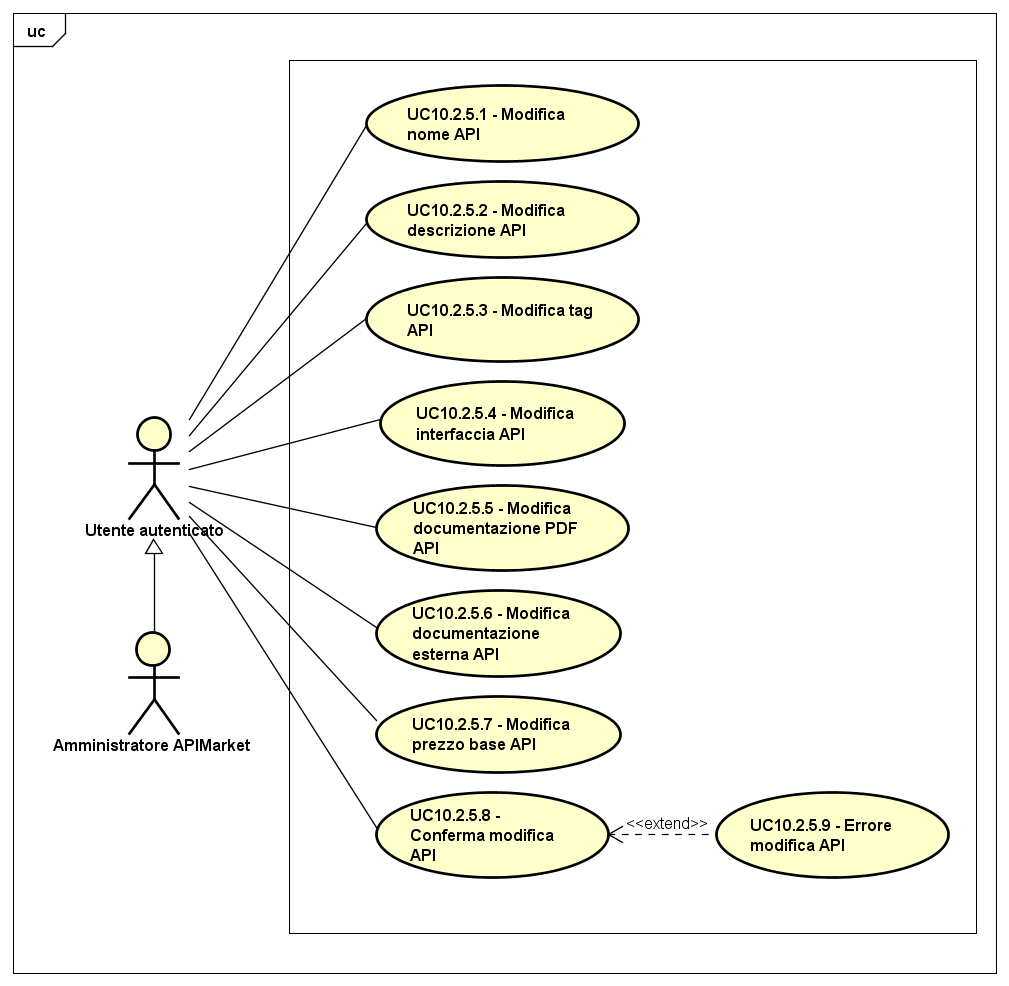
\includegraphics[scale=0.45]{UML/UC10_2_5.png}
	\caption{UC10.2.5: Modifica API registrata}
\end{figure}

\begin{minipage}{\linewidth}
	\begin{tabular}{ l | p{11cm}}
		\hline
		\rowcolor{Gray}
		\multicolumn{2}{c}{UC10.2.5 - Modifica API registrata} \\
		\hline
		\textbf{Attori} & Utente autenticato, Amministratore API Market \\
		\textbf{Descrizione} & L'attore modifica una API da lui registrata \\
		\textbf{Pre-Condizioni} & L'attore si trova nella schermata relativa alle API da lui registrate \\
		\textbf{Post-Condizioni} & L'attore ha modificato un API registrata \\
		\textbf{Scenario Principale} & 
		\begin{enumerate*}[label=(\arabic*.),itemjoin={\newline}]
			\item L'attore può modificare il nome dell'API (UC10.2.5.1)
			\item L'attore può modificare la descrizione dell'API (UC10.2.5.2)
			\item L'attore può modificare i tag dell'API (UC10.2.5.3)
			\item L'attore può modificare l'interfaccia dell'API (UC10.2.5.4)
			\item L'attore può modificare il file di documentazione PDF (UC10.2.5.5)
			\item L'attore può modificare il link alla documentazione esterna (UC10.2.5.6)
			\item L'attore può modificare il prezzo base dell'API (UC10.2.5.7)
			\item L'attore può confermare la modifica dell'API (UC10.2.5.8)
		\end{enumerate*}\\
		\textbf{Scenari Alternativi} & 
		\begin{enumerate*}[label=(\arabic*.),itemjoin={\newline}]
			\item L'attore può visualizzare un messaggio d'errore informativo e le modifiche non avvengono
		\end{enumerate*}\\
	\end{tabular}
\end{minipage}

\subparagraph{Caso d'uso UC10.2.5.1: Modifica nome API}
\label{UC10_2_5_1}

\begin{minipage}{\linewidth}
	\begin{tabular}{ l | p{11cm}}
		\hline
		\rowcolor{Gray}
		\multicolumn{2}{c}{UC10.2.5.1 - Modifica nome API} \\
		\hline
		\textbf{Attori} & Utente autenticato, Amministratore API Market \\
		\textbf{Descrizione} & L'attore modifica il nome dell'API \\
		\textbf{Pre-Condizioni} & L'attore si trova nella schermata relativa alla modifica di una API registrata, precedentemente selezionata \\
		\textbf{Post-Condizioni} & L'attore ha modificato il nome dell'API selezionata \\
		\textbf{Scenario Principale} & 
		\begin{enumerate*}[label=(\arabic*.),itemjoin={\newline}]
			\item L'attore può modificare il nome dell'API
		\end{enumerate*}\\
	\end{tabular}
\end{minipage}

\subparagraph{Caso d'uso UC10.2.5.2: Modifica descrizione API}
\label{UC10_2_5_2}

\begin{minipage}{\linewidth}
	\begin{tabular}{ l | p{11cm}}
		\hline
		\rowcolor{Gray}
		\multicolumn{2}{c}{UC10.2.5.2 - Modifica descrizione API} \\
		\hline
		\textbf{Attori} & Utente autenticato, Amministratore API Market \\
		\textbf{Descrizione} & L'attore modifica la descrizione dell'API\\
		\textbf{Pre-Condizioni} & L'attore si trova nella schermata relativa alla modifica di una API registrata, precedentemente selezionata \\
		\textbf{Post-Condizioni} & L'attore ha modificato la descrizione dell'API selezionata \\
		\textbf{Scenario Principale} & 
		\begin{enumerate*}[label=(\arabic*.),itemjoin={\newline}]
			\item L'attore può modificare la descrizione dell'API
		\end{enumerate*}\\
	\end{tabular}
\end{minipage}

\subparagraph{Caso d'uso UC10.2.5.3: Modifica tag API}
\label{UC10_2_5_3}

\begin{minipage}{\linewidth}
	\begin{tabular}{ l | p{11cm}}
		\hline
		\rowcolor{Gray}
		\multicolumn{2}{c}{UC10.2.5.3 - Modifica tag API} \\
		\hline
		\textbf{Attori} & Utente autenticato, Amministratore API Market \\
		\textbf{Descrizione} & L'attore modifica i tag dell'API \\
		\textbf{Pre-Condizioni} & L'attore si trova nella schermata relativa alla modifica di una API registrata, precedentemente selezionata \\
		\textbf{Post-Condizioni} & L'attore ha modificato i tag dell'API selezionata \\
		\textbf{Scenario Principale} & 
		\begin{enumerate*}[label=(\arabic*.),itemjoin={\newline}]
			\item L'attore può modificare i tag dell'API
		\end{enumerate*}\\
	\end{tabular}
\end{minipage}

\subparagraph{Caso d'uso UC10.2.5.4: Modifica interfaccia API}
\label{UC10_2_5_4}

\begin{minipage}{\linewidth}
	\begin{tabular}{ l | p{11cm}}
		\hline
		\rowcolor{Gray}
		\multicolumn{2}{c}{UC10.2.5.4 - Modifica interfaccia API} \\
		\hline
		\textbf{Attori} & Utente autenticato, Amministratore API Market \\
		\textbf{Descrizione} & L'attore modifica l'interfaccia dell'API \\
		\textbf{Pre-Condizioni} & L'attore si trova nella schermata relativa alla modifica di una API registrata, precedentemente selezionata \\
		\textbf{Post-Condizioni} & L'attore ha modificato l'interfaccia pubblica dell'API selezionata \\
		\textbf{Scenario Principale} & 
		\begin{enumerate*}[label=(\arabic*.),itemjoin={\newline}]
			\item L'attore può modificare l'interfaccia pubblica dell'API
		\end{enumerate*}\\
	\end{tabular}
\end{minipage}

\subparagraph{Caso d'uso UC10.2.5.5: Modifica documentazione PDF API}
\label{UC10_2_5_5}

\begin{minipage}{\linewidth}
	\begin{tabular}{ l | p{11cm}}
		\hline
		\rowcolor{Gray}
		\multicolumn{2}{c}{UC10.2.5.5 - Modifica documentazione PDF API} \\
		\hline
		\textbf{Attori} & Utente autenticato, Amministratore API Market \\
		\textbf{Descrizione} & L'attore modifica la documentazione PDF dell'API \\
		\textbf{Pre-Condizioni} & L'attore si trova nella schermata relativa alla modifica di una API registrata, precedentemente selezionata \\
		\textbf{Post-Condizioni} & L'attore ha modificato il file di documentazione dell'API selezionata \\
		\textbf{Scenario Principale} & 
		\begin{enumerate*}[label=(\arabic*.),itemjoin={\newline}]
			\item L'attore può selezionare un nuovo file dalle sue cartelle personali, che verrà caricato alla conferma
		\end{enumerate*}\\
		\textbf{Scenario Principale} & 
		\begin{enumerate*}[label=(\arabic*.),itemjoin={\newline}]
			\item Il file selezionato è di un formato non conforme e l'operazione non avviene
		\end{enumerate*}\\
	\end{tabular}
\end{minipage}

\subparagraph{Caso d'uso UC10.2.5.6: Modifica documentazione esterna API}
\label{UC10_2_5_6}

\begin{minipage}{\linewidth}
	\begin{tabular}{ l | p{11cm}}
		\hline
		\rowcolor{Gray}
		\multicolumn{2}{c}{UC10.2.5.6 - Modifica documentazione esterna API} \\
		\hline
		\textbf{Attori} & Utente autenticato, Amministratore API Market \\
		\textbf{Descrizione} & L'attore modifica la documentazione esterna dell'API \\
		\textbf{Pre-Condizioni} & L'attore si trova nella schermata relativa alla modifica di una API registrata, precedentemente selezionata \\
		\textbf{Post-Condizioni} & L'attore ha modificato il link di documentazione esterna dell'API selezionata \\
		\textbf{Scenario Principale} & 
		\begin{enumerate*}[label=(\arabic*.),itemjoin={\newline}]
			\item L'attore può modificare il link di documentazione esterna dell'API
		\end{enumerate*}\\
	\end{tabular}
\end{minipage}

\subparagraph{Caso d'uso UC10.2.5.7: Modifica prezzo base API}
\label{UC10_2_5_7}

\begin{minipage}{\linewidth}
	\begin{tabular}{ l | p{11cm}}
		\hline
		\rowcolor{Gray}
		\multicolumn{2}{c}{UC10.2.5.7 - Modifica prezzo base API} \\
		\hline
		\textbf{Attori} & Utente autenticato, Amministratore API Market \\
		\textbf{Descrizione} & L'attore modifica il prezzo base dell'API \\
		\textbf{Pre-Condizioni} & L'attore si trova nella schermata relativa alla modifica di una API registrata, precedentemente selezionata \\
		\textbf{Post-Condizioni} & L'attore ha modificato prezzo base dell'API selezionata \\
		\textbf{Scenario Principale} & 
		\begin{enumerate*}[label=(\arabic*.),itemjoin={\newline}]
			\item L'attore può modificare prezzo base dell'API
		\end{enumerate*}\\
	\end{tabular}
\end{minipage}

\subparagraph{Caso d'uso UC10.2.5.8: Conferma modifica API}
\label{UC10_2_5_8}

\begin{minipage}{\linewidth}
	\begin{tabular}{ l | p{11cm}}
		\hline
		\rowcolor{Gray}
		\multicolumn{2}{c}{UC10.2.5.8 - Conferma modifica API} \\
		\hline
		\textbf{Attori} & Utente autenticato, Amministratore API Market \\
		\textbf{Descrizione} & L'attore conferma le modifiche all'API, visualizzando un messaggio di successo \\
		\textbf{Pre-Condizioni} & L'attore si trova nella schermata relativa alla modifica di una API registrata, precedentemente selezionata \\
		\textbf{Post-Condizioni} & L'attore ha confermato le modifiche all'API, visualizzando un messaggio di successo \\
		\textbf{Scenario Principale} & 
		\begin{enumerate*}[label=(\arabic*.),itemjoin={\newline}]
			\item L'attore può confermare le modifiche effettuate all'API, visualizzando un messaggio di successo e venendo reindirizzato alla schermata di visualizzazione API registrate (UC10)
		\end{enumerate*}\\
	\end{tabular}
\end{minipage}

\subparagraph{Caso d'uso UC10.2.5.9: Errore modifica API}
\label{UC10_2_5_9}

\begin{minipage}{\linewidth}
	\begin{tabular}{ l | p{11cm}}
		\hline
		\rowcolor{Gray}
		\multicolumn{2}{c}{UC10.2.5.9 - Errore modifica API} \\
		\hline
		\textbf{Attori} & Utente autenticato, Amministratore API Market \\
		\textbf{Descrizione} & L'attore visualizza un messaggio di errore e la modifica non avviene \\
		\textbf{Pre-Condizioni} & L'attore ha confermato la modifica di una API ma si è verificato un errore \\
		\textbf{Post-Condizioni} & L'attore ha visualizzato un errore relativo alla modifica dell'API, con opportuna descrizione \\
		\textbf{Scenario Principale} & 
		\begin{enumerate*}[label=(\arabic*.),itemjoin={\newline}]
			\item L'attore può visualizzare un messaggio di errore e la modifica non avviene
		\end{enumerate*}\\
	\end{tabular}
\end{minipage}

\paragraph{Caso d'uso UC10.2.6: Eliminazione API registrata}
\label{UC10_2_6}

\begin{minipage}{\linewidth}
	\begin{tabular}{ l | p{11cm}}
		\hline
		\rowcolor{Gray}
		\multicolumn{2}{c}{UC10.2.6 - Eliminazione API registrata} \\
		\hline
		\textbf{Attori} & Utente autenticato, Amministratore API Market \\
		\textbf{Descrizione} & L'attore richiede l'eliminazione di una API da lui registrata, che verrà eliminata secondo le politiche di API Market \\
		\textbf{Pre-Condizioni} & L'attore si trova nella schermata relativa alle API da lui registrate \\
		\textbf{Post-Condizioni} & L'attore ha richiesto l'eliminazione di una API da lui registrata \\
		\textbf{Scenario Principale} & 
		\begin{enumerate*}[label=(\arabic*.),itemjoin={\newline}]
			\item L'attore può richiedere l'eliminazione di una API da lui registrata, che verrà eliminata secondo le politiche di API Market
		\end{enumerate*}\\
	\end{tabular}
\end{minipage}

\paragraph{Caso d'uso UC10.2.7: Revoca eliminazione API registrata}
\label{UC10_2_7}

\begin{minipage}{\linewidth}
	\begin{tabular}{ l | p{11cm}}
		\hline
		\rowcolor{Gray}
		\multicolumn{2}{c}{UC10.2.7 - Revoca eliminazione API registrata} \\
		\hline
		\textbf{Attori} & Utente autenticato, Amministratore API Market \\
		\textbf{Descrizione} & L'attore revoca la richiesta di eliminazione di una API da lui registrata \\
		\textbf{Pre-Condizioni} & L'attore si trova nella schermata relativa alle API da lui registrate \\
		\textbf{Post-Condizioni} & L'attore ha revocato la richiesta di eliminazione di una API da lui registrata \\
		\textbf{Scenario Principale} & 
		\begin{enumerate*}[label=(\arabic*.),itemjoin={\newline}]
			\item L'attore può revocare la richiesta di eliminazione di una API da lui registrata
		\end{enumerate*}\\
	\end{tabular}
\end{minipage}
\newpage
\subsection{Caso d'uso UC11 - Menù profilo utente}
\label{UC11}

\begin{figure}[ht]
	\centering
	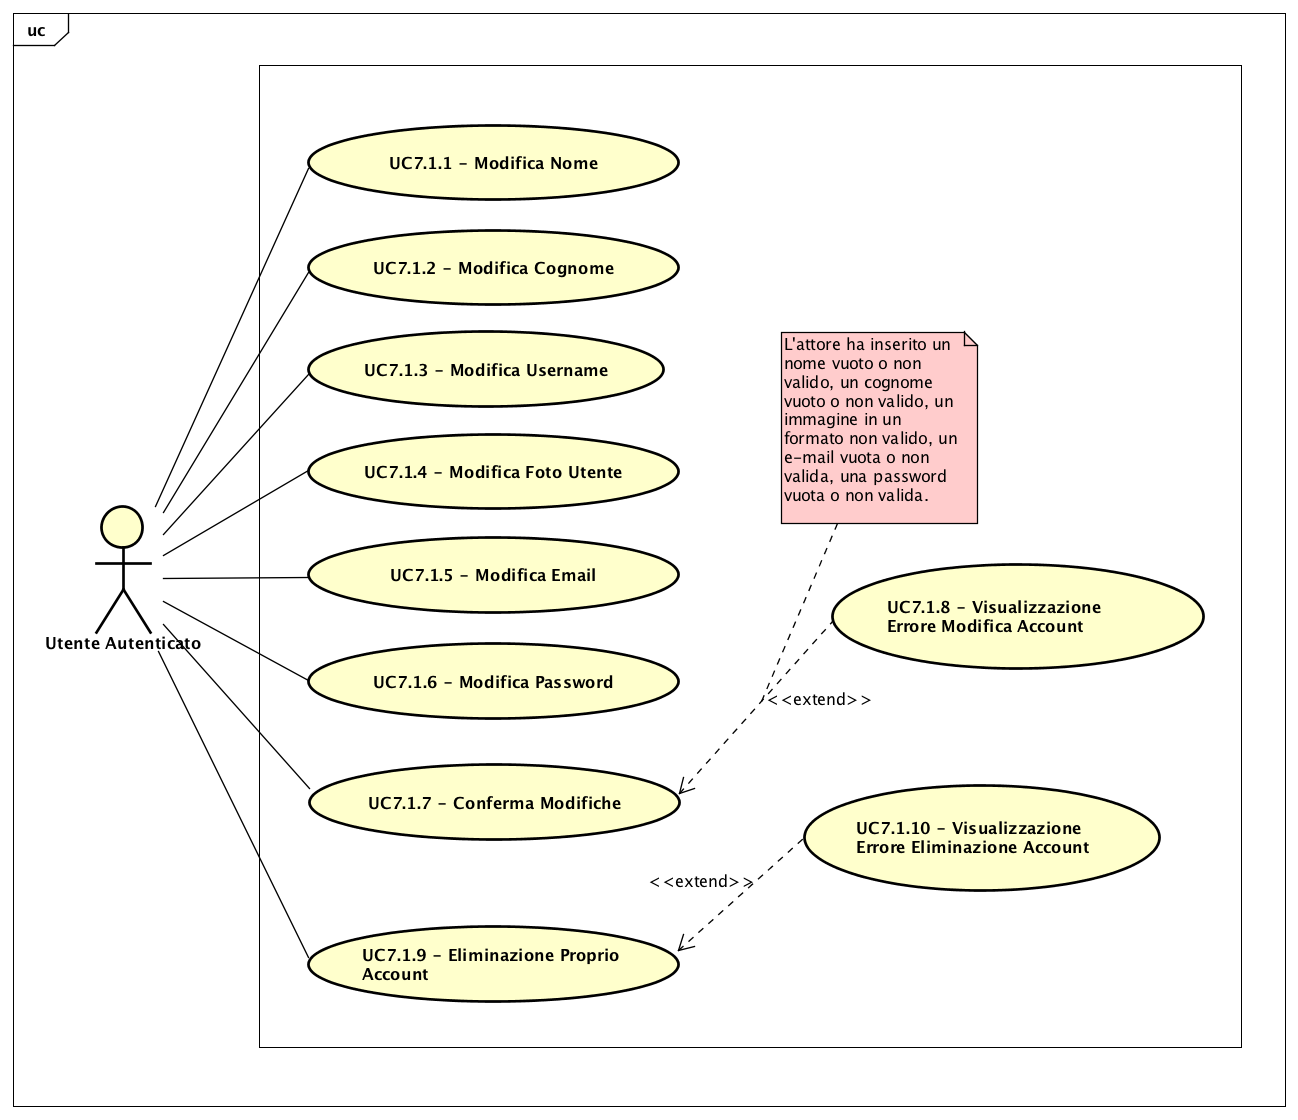
\includegraphics[scale=0.45]{UML/UC7_1.png}
	\caption{UC11 - Menù profilo utente}
\end{figure}
\FloatBarrier
\begin{longtable}{ l | p{11cm}}
	\hline
	\rowcolor{Gray}
	 \multicolumn{2}{c}{UC11 - Menù profilo utente} \\
	 \hline
	 \textbf{Attori} & Utente autenticato  \\
	\textbf{Descrizione} & L’attore può visualizzare e modificare i dati relativi all'account registrato \\
	\textbf{Pre-Condizioni} & L’attore è nel menù per la gestione del profilo \\
	\textbf{Post-Condizioni} & L’attore ha effettuato operazioni di gestione del proprio profilo \\
	\textbf{Scenario Principale} & 
	\begin{enumerate*}[label=(\arabic*.),itemjoin={\newline}]
		\item L'attore può gestire le proprie informazioni personali (UC11.1)
		\item L'attore può gestire il metodo di pagamento (UC11.2)
		\item L'attore può visualizzare le API acquistate (UC8)
		\item L'attore può interagire con le API da lui registrate e fornite sul marketplace (UCxx)
	\end{enumerate*}\\
\end{longtable}

\subsubsection{Caso d'uso UC11.1: Gestione informazioni personali}
\label{UC11_1}

\begin{minipage}{\linewidth}
	\begin{tabular}{ l | p{11cm}}
		\hline
		\rowcolor{Gray}
		\multicolumn{2}{c}{UC11.1 - Gestione informazioni personali} \\
		\hline
		\textbf{Attori} & Utente autenticato \\
		\textbf{Descrizione} & L'attore può gestire le proprie informazioni personali\\
		\textbf{Pre-Condizioni} & L'attore si trova nel menù relativo alla gestione delle informazioni personali del profilo\\
		\textbf{Post-Condizioni} & L'attore ha effettuato operazioni di gestione di informazioni personali \\
		\textbf{Scenario Principale} & 
		\begin{enumerate*}[label=(\arabic*.),itemjoin={\newline}]
			\item L'attore può visualizzare le informazioni personali (UC11.1.1)
			\item L'attore può modificare le informazioni personali (UC11.1.2)
		\end{enumerate*}
	\end{tabular}
\end{minipage}

\paragraph{Caso d'uso UC11.1.1: Visualizzazione info personali profilo utente}
\label{UC11_1_1}
\begin{figure}[ht]
	\centering
	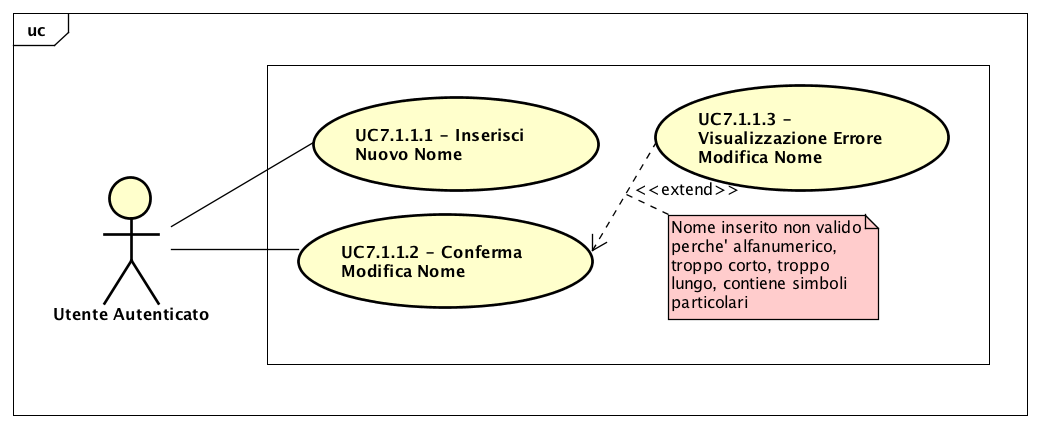
\includegraphics[scale=0.45]{UML/UC7_1_1.png}
	\caption{UC11.1.1: Visualizzazione info personali profilo utente}
\end{figure}
\FloatBarrier
\begin{tabular}{ l | p{11cm}}
	\hline
	\rowcolor{Gray}
	\multicolumn{2}{c}{UC11.1.1 - Visualizzazione info personali profilo utente} \\
	\hline
	\textbf{Attori} & Utente autenticato \\
	\textbf{Descrizione} & L'attore può visualizzare le informazioni personali relative al proprio account registrato\\
	\textbf{Pre-Condizioni} & L'attore è nella schermata di gestione informazioni personali\\
	\textbf{Post-Condizioni} & L'attore ha visualizzato le proprie informazioni personali \\
	\textbf{Scenario Principale} & 
	\begin{enumerate*}[label=(\arabic*.),itemjoin={\newline}]
		\item L'attore visualizza il nome (UC11.1.1.1)
		\item L'attore visualizza il cognome (UC11.1.1.2)
		\item L'attore visualizza lo username (UC11.1.1.3)
		\item L'attore visualizza l'email (UC11.1.1.4)
		\item L'attore visualizza l'immagine del profilo (UC11.1.1.5)
	\end{enumerate*}
\end{tabular}

\subparagraph{Caso d'uso UC11.1.1.1: Visualizzazione nome}
\label{UC11_1_1_1}
\begin{minipage}{\linewidth}
\begin{tabular}{ l | p{11cm}}
	\hline
	\rowcolor{Gray}
	\multicolumn{2}{c}{UC11.1.1.1 - Visualizzazione nome} \\
	\hline
	\textbf{Attori} & Utente autenticato \\
	\textbf{Descrizione} & L'attore può visualizzare il nome\\
	\textbf{Pre-Condizioni} & L'attore è nella schermata di visualizzazione informazioni personali\\
	\textbf{Post-Condizioni} & L'attore ha visualizzato il proprio nome \\
	\textbf{Scenario Principale} & 
	\begin{enumerate*}[label=(\arabic*.),itemjoin={\newline}]
		\item L'attore visualizza il proprio nome
	\end{enumerate*}
\end{tabular}
\end{minipage}

\subparagraph{Caso d'uso UC11.1.1.2: Visualizzazione cognome}
\label{UC11_1_1_2}
\begin{minipage}{\linewidth}
	\begin{tabular}{ l | p{11cm}}
		\hline
		\rowcolor{Gray}
		\multicolumn{2}{c}{UC11.1.1.2 - Visualizzazione cognome} \\
		\hline
		\textbf{Attori} & Utente autenticato \\
		\textbf{Descrizione} & L'attore può visualizzare il cognome\\
		\textbf{Pre-Condizioni} & L'attore è nella schermata di visualizzazione informazioni personali\\
		\textbf{Post-Condizioni} & L'attore ha visualizzato il proprio cognome \\
		\textbf{Scenario Principale} & 
		\begin{enumerate*}[label=(\arabic*.),itemjoin={\newline}]
			\item L'attore visualizza il proprio cognome
		\end{enumerate*}
	\end{tabular}
\end{minipage}

\subparagraph{Caso d'uso UC11.1.1.3: Visualizzazione username}
\label{UC11_1_1_3}
\begin{minipage}{\linewidth}
	\begin{tabular}{ l | p{11cm}}
		\hline
		\rowcolor{Gray}
		\multicolumn{2}{c}{UC11.1.1.3 - Visualizzazione username} \\
		\hline
		\textbf{Attori} & Utente autenticato \\
		\textbf{Descrizione} & L'attore può visualizzare lo username\\
		\textbf{Pre-Condizioni} & L'attore è nella schermata di visualizzazione informazioni personali\\
		\textbf{Post-Condizioni} & L'attore ha visualizzato il proprio username \\
		\textbf{Scenario Principale} & 
		\begin{enumerate*}[label=(\arabic*.),itemjoin={\newline}]
			\item L'attore visualizza il proprio username
		\end{enumerate*}
	\end{tabular}
\end{minipage}

\subparagraph{Caso d'uso UC11.1.1.4: Visualizzazione email}
\label{UC11_1_1_4}
\begin{minipage}{\linewidth}
	\begin{tabular}{ l | p{11cm}}
		\hline
		\rowcolor{Gray}
		\multicolumn{2}{c}{UC11.1.1.4 - Visualizzazione email} \\
		\hline
		\textbf{Attori} & Utente autenticato \\
		\textbf{Descrizione} & L'attore può visualizzare l'indirizzo email associato al proprio account\\
		\textbf{Pre-Condizioni} & L'attore è nella schermata di visualizzazione informazioni personali\\
		\textbf{Post-Condizioni} & L'attore ha visualizzato la propria email \\
		\textbf{Scenario Principale} & 
		\begin{enumerate*}[label=(\arabic*.),itemjoin={\newline}]
			\item L'attore visualizza la propria email
		\end{enumerate*}
	\end{tabular}
\end{minipage}

\subparagraph{Caso d'uso UC11.1.1.5: Visualizzazione immagine del profilo}
\label{UC11_1_1_5}
\begin{minipage}{\linewidth}
	\begin{tabular}{ l | p{11cm}}
		\hline
		\rowcolor{Gray}
		\multicolumn{2}{c}{UC11.1.1.5 - Visualizzazione immagine del profilo} \\
		\hline
		\textbf{Attori} & Utente autenticato \\
		\textbf{Descrizione} & L'attore può visualizzare l'immagine del profilo\\
		\textbf{Pre-Condizioni} & L'attore è nella schermata di visualizzazione informazioni personali\\
		\textbf{Post-Condizioni} & L'attore ha visualizzato l'immagine del proprio profilo \\
		\textbf{Scenario Principale} & 
		\begin{enumerate*}[label=(\arabic*.),itemjoin={\newline}]
			\item L'attore visualizza l'immagine del proprio profilo
		\end{enumerate*}
	\end{tabular}
\end{minipage}

\paragraph{Caso d'uso UC11.1.2: Modifica info personali profilo utente}
\label{UC11_1_2}
\begin{figure}[ht]
	\centering
	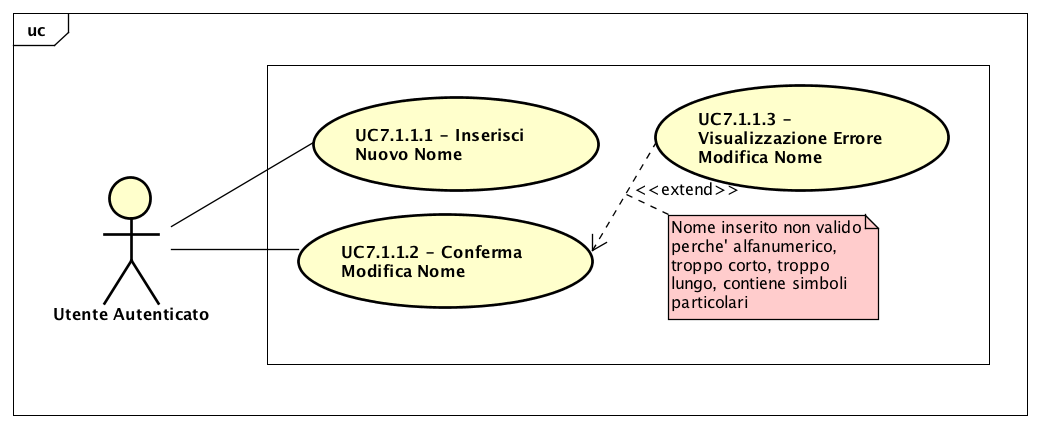
\includegraphics[scale=0.45]{UML/UC7_1_1.png}
	\caption{UC11.1.2: Modifica info personali profilo utente}
\end{figure}
\FloatBarrier
\begin{tabular}{ l | p{11cm}}
	\hline
	\rowcolor{Gray}
	\multicolumn{2}{c}{UC11.1.2 - Modifica info personali profilo utente} \\
	\hline
	\textbf{Attori} & Utente autenticato \\
	\textbf{Descrizione} & L'attore può modificare le informazioni personali relative al proprio profilo utente\\
	\textbf{Pre-Condizioni} & L'attore è nella schermata di gestione informazioni personali\\
	\textbf{Post-Condizioni} & L'attore ha modificato le proprie informazioni personali \\
	\textbf{Scenario Principale} & 
	\begin{enumerate*}[label=(\arabic*.),itemjoin={\newline}]
		\item L'attore può modificare il nome (UC11.1.2.1)
		\item L'attore può modificare il cognome (UC11.1.2.2)
		\item L'attore può modificare lo username (UC11.1.2.3)
		\item L'attore può modificare l'email (UC11.1.2.4)
		\item L'attore può modificare l'immagine del profilo (UC11.1.2.4)
		\item L'attore può confermare le modifiche effettuate (UC11.1.2.5)
	\end{enumerate*}\\
	\textbf{Scenari Alternativi} & 
	\begin{enumerate*}[label=(\arabic*.),itemjoin={\newline}]
		\item L'attore visualizza gli errori rilevati nelle modifiche richieste (UC)
	\end{enumerate*}\\
\end{tabular}

\subparagraph{Caso d'uso UC11.1.2.1: Modifica nome}
\label{UC11_1_2_1}
\begin{minipage}{\linewidth}
	\begin{tabular}{ l | p{11cm}}
		\hline
		\rowcolor{Gray}
		\multicolumn{2}{c}{UC11.1.2.1 - Modifica nome} \\
		\hline
		\textbf{Attori} & Utente autenticato \\
		\textbf{Descrizione} & L'attore può modificare il nome\\
		\textbf{Pre-Condizioni} & L'attore è nella schermata di modifica informazioni personali\\
		\textbf{Post-Condizioni} & L'attore ha modificato il nome \\
		\textbf{Scenario Principale} & 
		\begin{enumerate*}[label=(\arabic*.),itemjoin={\newline}]
			\item L'attore inserisce il nuovo nome
			\item L'attore conferma l'inserimento del nuovo nome
		\end{enumerate*}\\
		\textbf{Scenari Alternativi} & 
		\begin{enumerate*}[label=(\arabic*.),itemjoin={\newline}]
			\item L'attore visualizza un errore dovuto all'inserimento di un nome non consono
		\end{enumerate*}
	\end{tabular}
\end{minipage}

\subparagraph{Caso d'uso UC11.1.2.2: Modifica cognome}
\label{UC11_1_2_2}
\begin{minipage}{\linewidth}
	\begin{tabular}{ l | p{11cm}}
		\hline
		\rowcolor{Gray}
		\multicolumn{2}{c}{UC11.1.2.2 - Modifica cognome} \\
		\hline
		\textbf{Attori} & Utente autenticato \\
		\textbf{Descrizione} & L'attore può modificare il cognome\\
		\textbf{Pre-Condizioni} & L'attore è nella schermata di modifica informazioni personali\\
		\textbf{Post-Condizioni} & L'attore ha modificato il cognome \\
		\textbf{Scenario Principale} & 
		\begin{enumerate*}[label=(\arabic*.),itemjoin={\newline}]
			\item L'attore inserisce il nuovo cognome
			\item L'attore conferma l'inserimento del nuovo cognome
		\end{enumerate*}\\
		\textbf{Scenari Alternativi} & 
		\begin{enumerate*}[label=(\arabic*.),itemjoin={\newline}]
			\item L'attore visualizza un errore dovuto all'inserimento di un cognome non consono
		\end{enumerate*}
	\end{tabular}
\end{minipage}

\subsubsection{Caso d'uso UC11.2: Gestione metodo di pagamento}
\label{UC11_2}

\begin{minipage}{\linewidth}
	\begin{tabular}{ l | p{11cm}}
		\hline
		\rowcolor{Gray}
		\multicolumn{2}{c}{UC11.2 - Gestione metodo di pagamento} \\
		\hline
		\textbf{Attori} & Utente autenticato \\
		\textbf{Descrizione} & L'attore può gestire il proprio credito \\
		\textbf{Pre-Condizioni} & L'attore si trova nel menù relativo alla gestione del metodo di pagamento\\
		\textbf{Post-Condizioni} & L'attore ha effettuato operazioni relative al metodo di pagamento \\
		\textbf{Scenario Principale} & 
		\begin{enumerate*}[label=(\arabic*.),itemjoin={\newline}]
			\item L'attore può visualizzare il credito attuale presente nel proprio account (UC11.2.1)
			\item L'attore può effettuare un versamento per accrescere il proprio credito (UC11.2.2)
		\end{enumerate*}
	\end{tabular}
\end{minipage}


%\newpage
\subsection{Caso d'uso UC7 - Visualizzazione API}
\label{UC7}
\begin{figure}[ht]
	\centering
	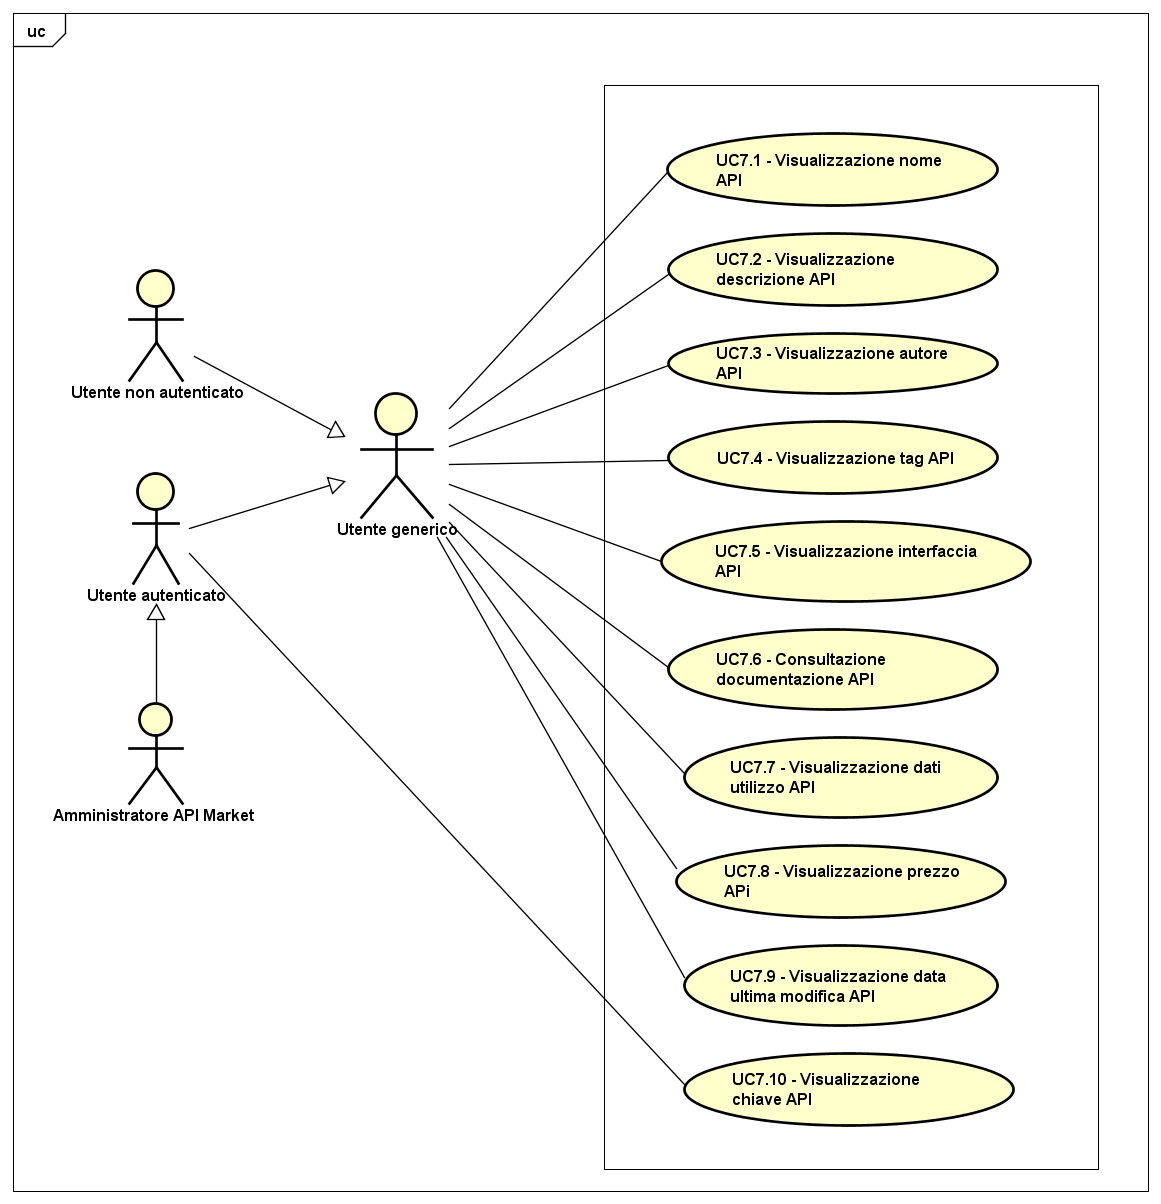
\includegraphics[scale=0.45]{UML/UC7.png}
	\caption{UC7: Visualizzazione API}
\end{figure}

\begin{longtable}{ l | p{11cm}}
	\hline
	\rowcolor{Gray}
	\multicolumn{2}{c}{UC7 - Visualizzazione API}\\
	\hline
	
	 \textbf{Attori} & Utente non autenticato, Utente autenticato  \\
	\textbf{Descrizione} & L'attore può visualizzare i dati relativi a un API che ha selezionato tramite la homepage o i risultati di una ricerca  \\
	\textbf{Pre-Condizioni} & L'attore ha selezionato un prodotto per la consultazione \\
	\textbf{Post-Condizioni} & L'attore visualizza la pagina relativa all'API selezionata\\
	\textbf{Scenario Principale} & 
	\begin{enumerate*}[label=(\arabic*.),itemjoin={\newline}]
		\item L'attore visualizza il nome dell'API (UC7.1)
		\item L'attore visualizza la descrizione dell'API (UC7.2)
		\item L'attore visualizza l'autore dell'API (UC7.3)
		\item L'attore può visualizzare l'interfaccia dell'API (UC7.4)
		\item L'attore può consultare la documentazione fornita dall'utente (UC7.5)
		\item L'utente può visualizzare i dati di utilizzo dell'API  (UC7.6)
	\end{enumerate*}\\
\end{longtable}

%\newpage
\subsubsection{UC7.1 - Gestione Proprio Profilo Utente}
\label{UC7.1}

\begin{figure}[ht]
	\centering
	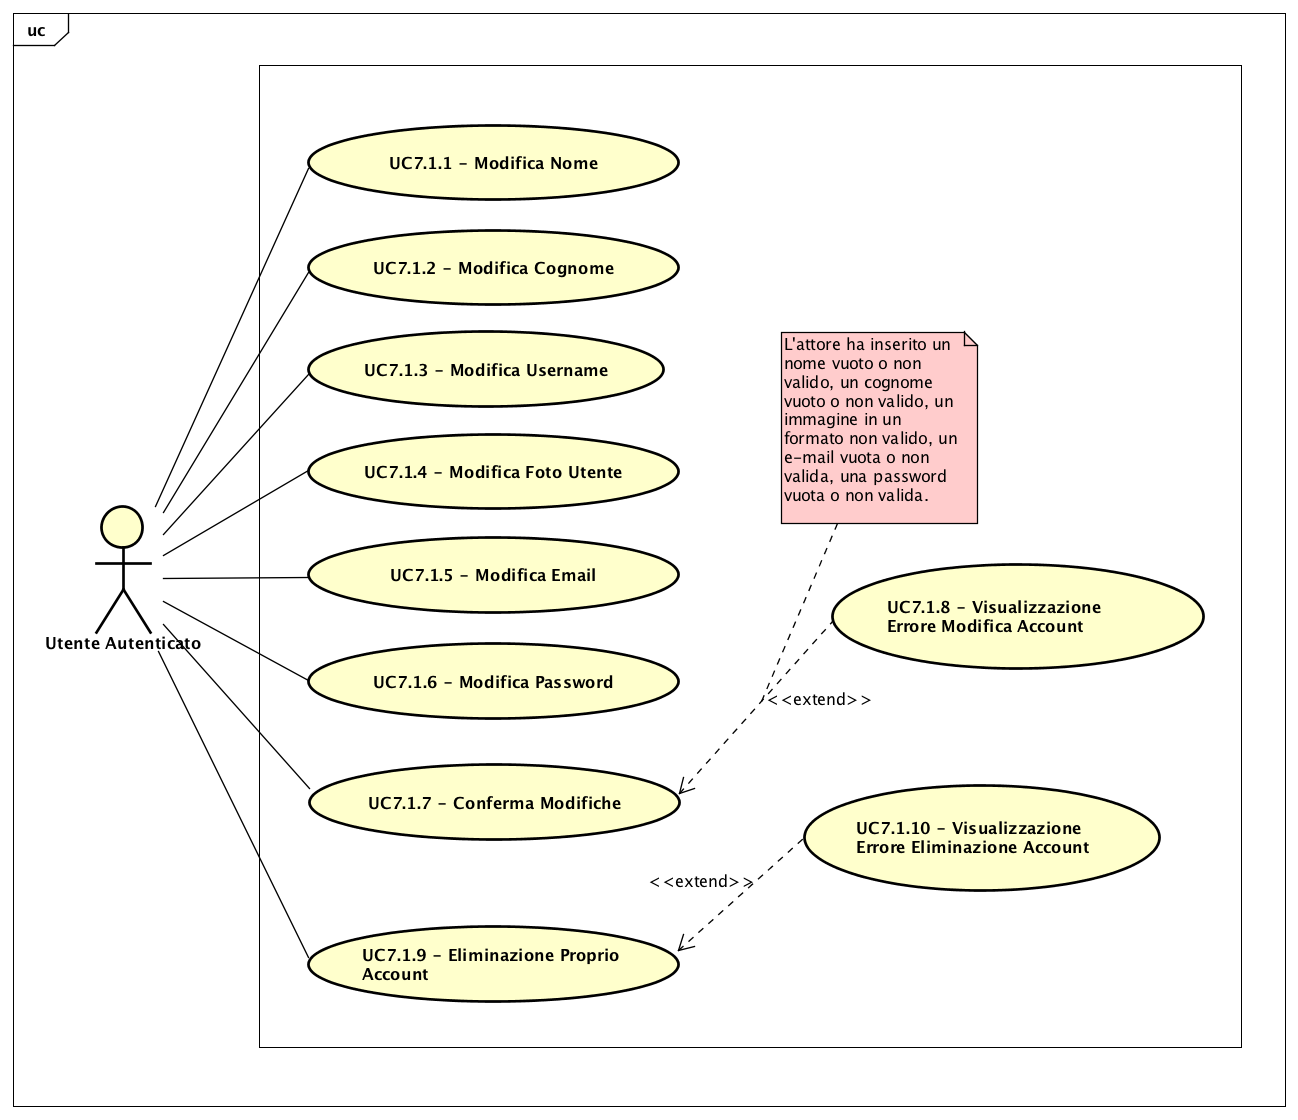
\includegraphics[scale=0.45]{UML/UC7_1.png}
	\caption{UC7.1 - Gestione Proprio Profilo Utente}
\end{figure}
\FloatBarrier
\begin{longtable}{ l | p{11cm}}
	\hline
	\rowcolor{Gray}
	 \multicolumn{2}{c}{UC7.1 - Gestione Proprio Profilo Utente} \\
	 \hline
	 \textbf{Attori} & Utente autenticato  \\
	\textbf{Descrizione} & L’utente pu\'{o} modificare le proprie informazioni personali  \\
	\textbf{Pre-Condizioni} & L’Utente \`{e} nel proprio profilo \\
	\textbf{Post-Condizioni} & L’Utente ha aggiornato il proprio profilo \\
	\textbf{Scenario Principale} & 
	\begin{enumerate*}[label=(\arabic*.),itemjoin={\newline}]
		\item L'utente pu\`{o} modificare il Nome (UC7.1.1)
		\item L'utente pu\`{o} modificare il Cognome (UC7.1.2)
		\item L'utente pu\`{o} modificare l'Username (UC7.1.3)
		\item L'utente pu\`{o} modificare la Foto Utente (UC7.1.4)
		\item L'utente pu\`{o} modificare l'Email (UC7.1.5)
		\item L'utente pu\`{o} modificare la Password (UC7.1.6)
		\item L'utente pu\`{o} confermare le Proprie Modifiche (UC7.1.7)
		\item L'utente pu\`{o} eliminare il Proprio Account (UC7.1.9)
	\end{enumerate*}\\
	\textbf{Scenari Alternativi} & 
		\begin{enumerate*}[label=(\arabic*.),itemjoin={\newline}]
		\item L'utente visualizza un Errore di Modifica Account se le modifiche risultano illegali (UC7.1.8)
		\item L'utente visualizza un Errore di Modifica Account se risulta un errore durante eliminazione (UC7.1.10)
	\end{enumerate*}\\
\end{longtable}




%\paragraph{Caso d'uso UC7.1.1:  Modifica Nome}
\label{UC7_1_1}
\begin{figure}[ht]
	\centering
	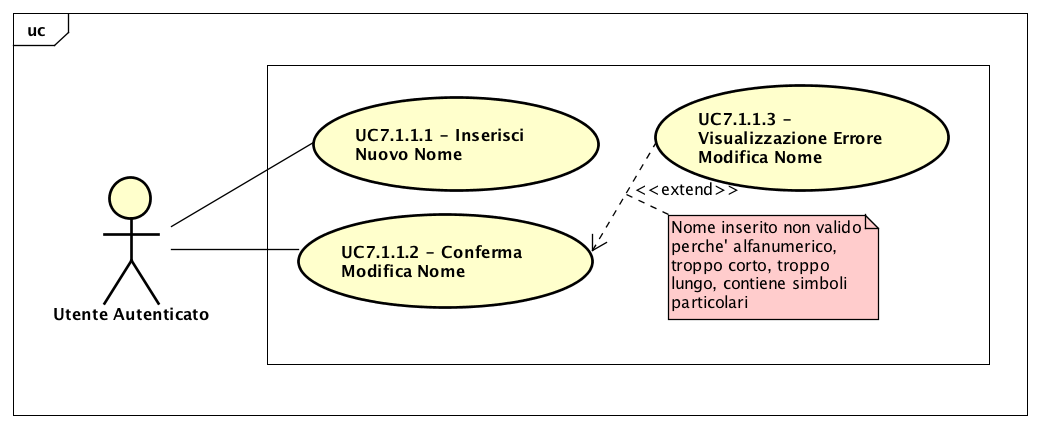
\includegraphics[scale=0.45]{UML/UC7_1_1.png}
	\caption{UC7.1.1:  Modifica Nome}
\end{figure}
\FloatBarrier
\begin{tabular}{ l | p{11cm}}
	\hline
	\rowcolor{Gray}
	 \multicolumn{2}{c}{UC7.1.1 - Modifica Nome} \\
	 \hline
	\textbf{Attori} & Utente Autenticato \\
	\textbf{Descrizione} & Gli utenti possono modificare il proprio Nome\\
	\textbf{Pre-Condizioni} & L'utente e' nella schermata di gestione Profilo\\
	\textbf{Post-Condizioni} & L'utente ha modificato con successo il proprio Nome \\
	\textbf{Scenario Principale} & 
	\begin{enumerate*}[label=(\arabic*.),itemjoin={\newline}]
		\item L'utente puo' inserire il Nuovo Nome (UC7.1.1.1)
		\item L'utente conferma la modifica al Nome (UC7.1.1.2)
	\end{enumerate*}\\
	\textbf{Scenari Alternativi} & 
	\begin{enumerate*}[label=(\arabic*.),itemjoin={\newline}]
		\item L'utente visualizza un errore nella modifica del Nome (UC7.1.1.3)
	\end{enumerate*}\\
\end{tabular}

%\subparagraph{Caso d'uso UC7.1.1.1:  Inserimento Nuovo Nome}
\label{UC7_1_1_1}

\begin{tabular}{ l | p{11cm}}
	\hline
	\rowcolor{Gray}
	 \multicolumn{2}{c}{UC7.1.1.1 - Inserimento Nuovo Nome} \\
	 \hline
	\textbf{Attori} & Utente Autenticato \\
	\textbf{Descrizione} & L'utente inserisce un nuovo Nome\\
	\textbf{Pre-Condizioni} & L'utente e' nella processo di modifica del Nome\\
	\textbf{Post-Condizioni} & L'utente ha scritto un nuovo Nome nell'editor\\
	\textbf{Scenario Principale} & 
	\begin{enumerate*}[label=(\arabic*.),itemjoin={\newline}]
		\item L'utente scrive un nuovo nome 
	\end{enumerate*}\\
\end{tabular}
%\subparagraph{Caso d'uso UC7.1.1.2:  Conferma Modifica Nome}
\label{UC7_1_1_2}

\begin{tabular}{ l | p{11cm}}
	\hline
	\rowcolor{Gray}
	 \multicolumn{2}{c}{UC7.1.1.2 - Conferma Modifica Nome} \\
	 \hline
	\textbf{Attori} & Utente Autenticato \\
	\textbf{Descrizione} & L'utente conferma il Nuovo Nome inserito\\
	\textbf{Pre-Condizioni} & L'utente ha scritto il proprio nome in Input\\
	\textbf{Post-Condizioni} & L'utente ha modificato il proprio Nome\\
	\textbf{Scenario Principale} & 
	\begin{enumerate*}[label=(\arabic*.),itemjoin={\newline}]
		\item L'utente conferma il nuovo Nome inserito
	\end{enumerate*}\\
	\textbf{Scenari Alternativi} & 
	\begin{enumerate*}[label=(\arabic*.),itemjoin={\newline}]
		\item L'utente scritto contiene simboli particolari
	\end{enumerate*}\\
\end{tabular}
%\paragraph{Caso d'uso UC7.1.2:  Modifica Cognome}
\label{UC7_1_2}
\begin{figure}[ht]
	\centering
	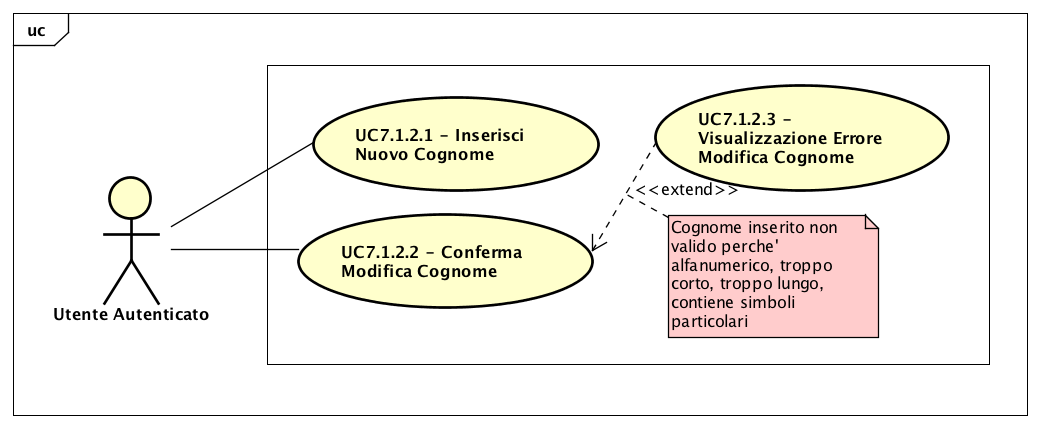
\includegraphics[scale=0.45]{UML/UC7_1_2.png}
	\caption{UC7.1.2:  Modifica Cognome}
\end{figure}

\FloatBarrier
\begin{tabular}{ l | p{11cm}}
	\hline
	\rowcolor{Gray}
	 \multicolumn{2}{c}{UC7.1.2 - Modifica Cognome} \\
	 \hline
	\textbf{Attori} & Utente Autenticato \\
	\textbf{Descrizione} & Gli utenti possono modificare il proprio Cognome\\
	\textbf{Pre-Condizioni} & L'utente e' nella schermata di gestione Profilo\\
	\textbf{Post-Condizioni} & L'utente ha modificato con successo il proprio Cognome \\
	\textbf{Scenario Principale} & 
	\begin{enumerate*}[label=(\arabic*.),itemjoin={\newline}]
		\item L'utente puo' inserire il Nuovo Cognome (UC7.1.2.1)
		\item L'utente conferma la modifica al Cognome (UC7.1.2.2)
	\end{enumerate*}\\
	\textbf{Scenari Alternativi} & 
	\begin{enumerate*}[label=(\arabic*.),itemjoin={\newline}]
		\item L'utente visualizza un errore nella modifica del Cognome (UC7.1.2.3)
	\end{enumerate*}\\
\end{tabular}

%\subparagraph{Caso d'uso UC7.1.2.1:  Inserimento Nuovo Cognome}
\label{UC7_1_2_1}

\begin{tabular}{ l | p{11cm}}
	\hline
	\rowcolor{Gray}
	 \multicolumn{2}{c}{UC7.1.2.1 - Inserimento Nuovo Cognome} \\
	 \hline
	\textbf{Attori} & Utente Autenticato \\
	\textbf{Descrizione} & L'utente inserisce un nuovo Cognome in Input\\
	\textbf{Pre-Condizioni} & L'utente e' nella processo di modifica del Cognome\\
	\textbf{Post-Condizioni} & L'utente ha scritto un nuovo Nome nell'editor\\
	\textbf{Scenario Principale} & 
	\begin{enumerate*}[label=(\arabic*.),itemjoin={\newline}]
		\item L'utente scrive un nuovo Cognome (UC7.1.1.1)
	\end{enumerate*}\\
\end{tabular}
%\subparagraph{Caso d'uso UC7.1.2.2:  Conferma Modifica Cognome}
\label{UC7_1_2_2}

\begin{tabular}{ l | p{11cm}}
	\hline
	\rowcolor{Gray}
	 \multicolumn{2}{c}{UC7.1.2.2:  Conferma Modifica Cognome} \\
	 \hline
	\textbf{Attori} & Utente Autenticato \\
	\textbf{Descrizione} & L'utente inserisce un nuovo nome\\
	\textbf{Pre-Condizioni} & L'utente e' nella schermata di gestione Profilo\\
	\textbf{Post-Condizioni} & L'utente ha scritto un nuovo Cognome nell'editor\\
	\textbf{Scenario Principale} & 
	\begin{enumerate*}[label=(\arabic*.),itemjoin={\newline}]
		\item L'utente conferma il nuovo Cognome (UC7.1.1.1)
	\end{enumerate*}\\
\end{tabular}
%\paragraph{Caso d'uso UC7.1.3:  Modifica Username}
\label{UC7_1_3}
\begin{figure}[ht]
	\centering
	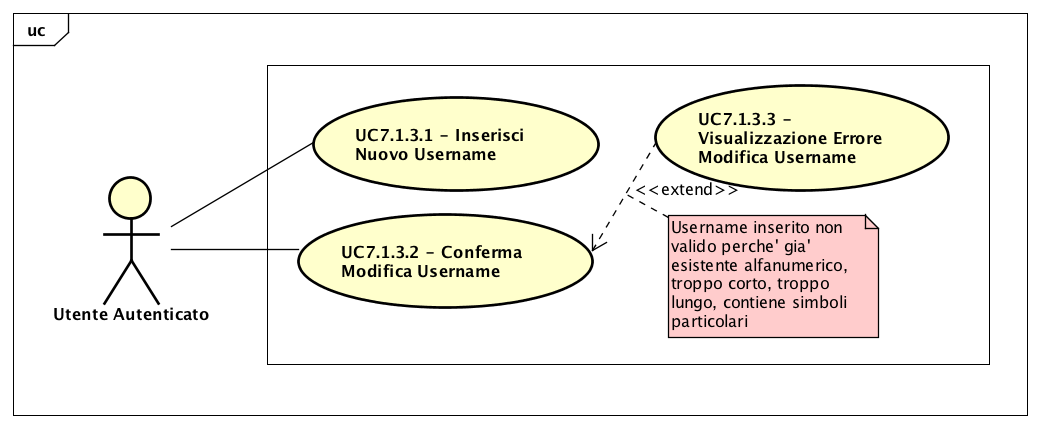
\includegraphics[scale=0.45]{UML/UC7_1_3.png}
	\caption{UC7.1.3:  Modifica Username}
\end{figure}
\FloatBarrier
\begin{tabular}{ l | p{11cm}}
	\hline
	\rowcolor{Gray}
	 \multicolumn{2}{c}{UC7.1.3 - Modifica Username} \\
	 \hline
		\textbf{Attori} & Utente Autenticato \\
	\textbf{Descrizione} & Gli utenti possono modificare il proprio Username\\
	\textbf{Pre-Condizioni} & L'utente e' nella schermata di gestione Profilo\\
	\textbf{Post-Condizioni} & L'utente ha modificato con successo il proprio Username \\
	\textbf{Scenario Principale} & 
	\begin{enumerate*}[label=(\arabic*.),itemjoin={\newline}]
		\item L'utente puo' inserire il Nuovo Username (UC7.1.3.1)
		\item L'utente conferma la modifica al Username (UC7.1.3.2)
	\end{enumerate*}\\
	\textbf{Scenari Alternativi} & 
	\begin{enumerate*}[label=(\arabic*.),itemjoin={\newline}]
		\item L'utente visualizza un errore nella modifica del Username (UC7.1.3.3)
	\end{enumerate*}\\
\end{tabular}

%\subparagraph{Caso d'uso UC7.1.3.1:  Inserimento Nuovo Username}
\label{UC7_1_3_1}

\begin{tabular}{ l | p{11cm}}
	\hline
	\rowcolor{Gray}
	 \multicolumn{2}{c}{UC7.1.3.1:  Inserimento Nuovo Username} \\
	 \hline
	\textbf{Attori} & Utente Autenticato \\
	\textbf{Descrizione} & L'utente inserisce un nuovo Username\\
	\textbf{Pre-Condizioni} & L'utente e' nella processo di modifica del Username\\
	\textbf{Post-Condizioni} & L'utente ha scritto un nuovo Username nell'editor\\
	\textbf{Scenario Principale} & 
	\begin{enumerate*}[label=(\arabic*.),itemjoin={\newline}]
		\item L'utente scrive un nuovo Username
	\end{enumerate*}\\
\end{tabular}
%\subparagraph{Caso d'uso UC7.1.3.2:  Conferma Modifica Username}
\label{UC7_1_3_2}

\begin{tabular}{ l | p{11cm}}
	\hline
	\rowcolor{Gray}
	 \multicolumn{2}{c}{UC7.1.3.2 - Conferma Modifica Username} \\
	 \hline
	\textbf{Attori} & Utente Autenticato \\
	\textbf{Descrizione} & L'utente conferma l'username\\
	\textbf{Pre-Condizioni} & L'utente ha scritto un nuovo username nell'editor\\
	\textbf{Post-Condizioni} & L'utente ha modificato l'username\\
	\textbf{Scenario Principale} & 
	\begin{enumerate*}[label=(\arabic*.),itemjoin={\newline}]
		\item L'utente conferma il nuovo username appena scritto
	\end{enumerate*}\\
\end{tabular}
%\paragraph{Caso d'uso UC7.1.4:  Modifica Foto Utente}
\label{UC7_1_4}
\begin{figure}[ht]
	\centering
	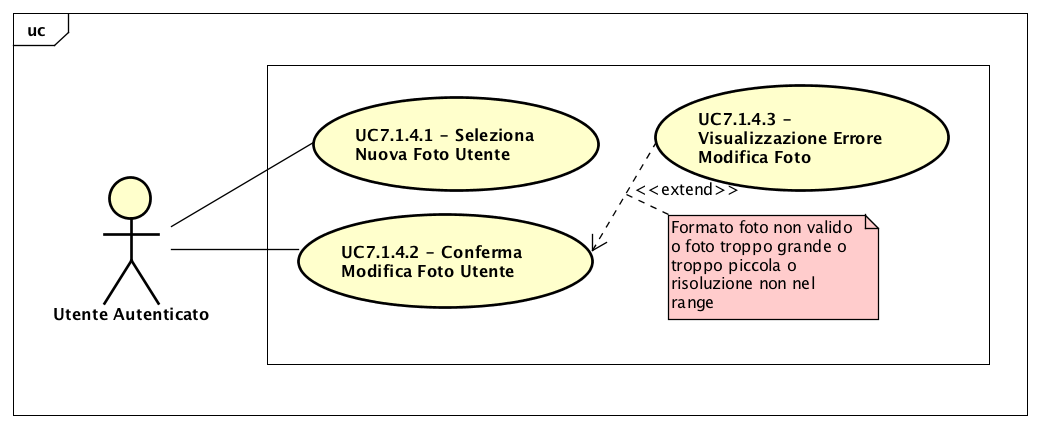
\includegraphics[scale=0.45]{UML/UC7_1_4.png}
	\caption{UC4: Login}
\end{figure}
\FloatBarrier
\begin{tabular}{ l | p{11cm}}
	\hline
	\rowcolor{Gray}
	 \multicolumn{2}{c}{UC7.1.4 - Modifica Foto Utente} \\
	 \hline
		\textbf{Attori} & Utente Autenticato \\
	\textbf{Descrizione} & Gli utenti possono modificare la propria Foto Profilo Utente selezionandola dal loro dispositivo\\
	\textbf{Pre-Condizioni} & L'utente e' nella schermata di gestione Profilo\\
	\textbf{Post-Condizioni} & L'utente ha modificato con successo la propria Foto Profilo \\
	\textbf{Scenario Principale} & 
	\begin{enumerate*}[label=(\arabic*.),itemjoin={\newline}]
		\item L'utente puo' inserire selezionare una Nuova Foto (UC7.1.4.1)
		\item L'utente conferma la modifica alla Foto Profilo (UC7.1.2.2)
	\end{enumerate*}\\
	\textbf{Scenari Alternativi} & 
	\begin{enumerate*}[label=(\arabic*.),itemjoin={\newline}]
		\item L'utente visualizza un errore nella modifica della Foto (UC7.1.2.3)
	\end{enumerate*}\\
\end{tabular}

%\subparagraph{Caso d'uso UC7.1.4.1:  Seleziona Nuova Foto Utente}
\label{UC7_1_4_1}

\begin{tabular}{ l | p{11cm}}
	\hline
	\rowcolor{Gray}
	 \multicolumn{2}{c}{UC7.1.4.1:  Seleziona Nuova Foto Utente} \\
	 \hline
	\textbf{Attori} & Utente Autenticato \\
	\textbf{Descrizione} & L'attore sceglie una Nuova Foto Utente localmente\\
	\textbf{Pre-Condizioni} & L'utente e' nella processo di modifica della Foto Utente\\
	\textbf{Post-Condizioni} & L'utente ha scelto una Nuova Foto Utente\\
	\textbf{Scenario Principale} & 
	\begin{enumerate*}[label=(\arabic*.),itemjoin={\newline}]
		\item L'utente sceglie una foto 
	\end{enumerate*}\\
\end{tabular}
%\subparagraph{Caso d'uso UC7.1.4.2:  Conferma Modifica Foto Utente}
\label{UC7_1_4_2}

\begin{tabular}{ l | p{11cm}}
	\hline
	\rowcolor{Gray}
	 \multicolumn{2}{c}{UC7.1.4.2:  Conferma Modifica Foto Utente} \\
	 \hline
	\textbf{Attori} & Utente Autenticato \\
	\textbf{Descrizione} & L'utente conferma la modifica alla foto\\
	\textbf{Pre-Condizioni} & L'utente ha scelto una foto utente\\
	\textbf{Post-Condizioni} & L'utente ha modificato con successo la propria foto\\
	\textbf{Scenario Principale} & 
	\begin{enumerate*}[label=(\arabic*.),itemjoin={\newline}]
		\item L'utente conferma la modifica della foto
	\end{enumerate*}\\
\end{tabular}
%\paragraph{Caso d'uso UC7.1.5:  Modifica Email}
\label{UC7_1_5}
\begin{figure}[ht]
	\centering
	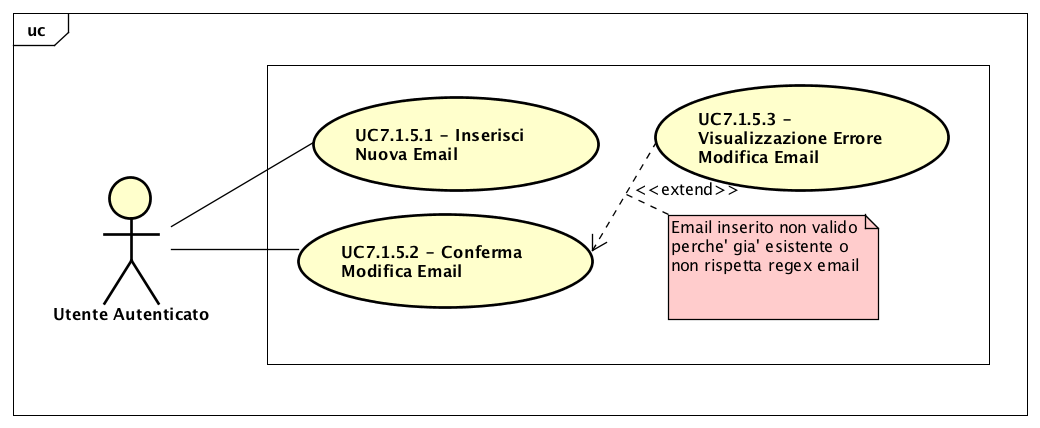
\includegraphics[scale=0.45]{UML/UC7_1_5.png}
	\caption{UC7.1.5:  Modifica Email}
\end{figure}
\FloatBarrier
\begin{tabular}{ l | p{11cm}}
	\hline
	\rowcolor{Gray}
	 \multicolumn{2}{c}{UC7.1.5 - Modifica Email} \\
	 \hline
		\textbf{Attori} & Utente Autenticato \\
	\textbf{Descrizione} & Gli utenti possono modificare la propria Email\\
	\textbf{Pre-Condizioni} & L'utente e' nella schermata di gestione Profilo\\
	\textbf{Post-Condizioni} & L'utente ha modificato con successo la Propria Email\\
	\textbf{Scenario Principale} & 
	\begin{enumerate*}[label=(\arabic*.),itemjoin={\newline}]
		\item L'utente puo' inserire la nuova Email (UC7.1.5.1)
		\item L'utente conferma la modifica al'Email (UC7.1.5.2)
	\end{enumerate*}\\
	\textbf{Scenari Alternativi} & 
	\begin{enumerate*}[label=(\arabic*.),itemjoin={\newline}]
		\item L'utente visualizza un errore nella modifica dell'Email (UC7.1.5.3)
	\end{enumerate*}\\
\end{tabular}


%\subparagraph{Caso d'uso UC7.1.5.1:  Inserimento Nuova Email}
\label{UC7_1_5_1}

\begin{tabular}{ l | p{11cm}}
	\hline
	\rowcolor{Gray}
	 \multicolumn{2}{c}{UC7.1.5.1 - Inserimento Nuova Email} \\
	 \hline
	\textbf{Attori} & Utente Autenticato \\
	\textbf{Descrizione} & L'utente inserisce un nuova Email nell'Editor\\
	\textbf{Pre-Condizioni} & L'utente e' nella Editor di modifica dell'Email\\
	\textbf{Post-Condizioni} & L'utente ha scritto una nuova Email nell'Editor\\
	\textbf{Scenario Principale} & 
	\begin{enumerate*}[label=(\arabic*.),itemjoin={\newline}]
		\item L'utente scrive una nuova Email
	\end{enumerate*}\\
\end{tabular}
%\subparagraph{Caso d'uso UC7.1.5.2:  Conferma Modifica Email}
\label{UC7_1_5_2}

\begin{tabular}{ l | p{11cm}}
	\hline
	\rowcolor{Gray}
	 \multicolumn{2}{c}{UC7.1.5.2:  Conferma Modifica Email} \\
	 \hline
	\textbf{Attori} & Utente Autenticato \\
	\textbf{Descrizione} & L'utente inserisce un nuovo nome\\
	\textbf{Pre-Condizioni} & L'utente e' nella schermata di gestione Profilo\\
	\textbf{Post-Condizioni} & L'utente ha scritto un nuovo Nome nell'editor\\
	\textbf{Scenario Principale} & 
	\begin{enumerate*}[label=(\arabic*.),itemjoin={\newline}]
		\item L'utente scrive un nuovo nome (UC7.1.1.1)
	\end{enumerate*}\\
\end{tabular}
%\paragraph{Caso d'uso UC7.1.6:  Modifica Password}
\label{UC7_1_6}
\begin{figure}[ht]
	\centering
	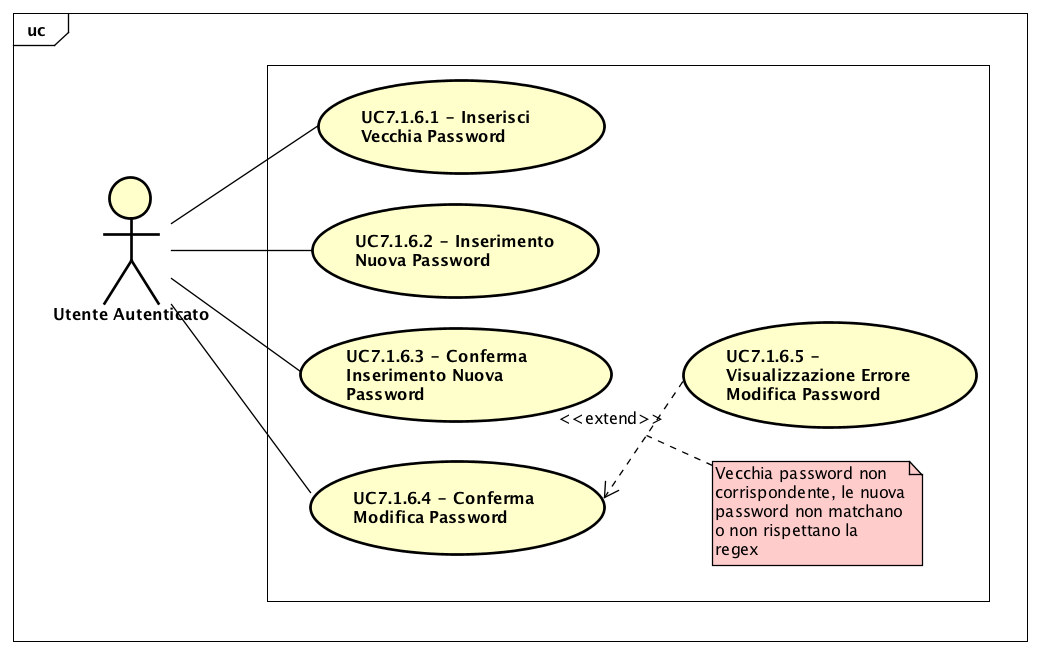
\includegraphics[scale=0.45]{UML/UC7_1_6.png}
	\caption{UC7.1.6:  Modifica Password}
\end{figure}
\FloatBarrier
\begin{tabular}{ l | p{11cm}}
	\hline
	\rowcolor{Gray}
	 \multicolumn{2}{c}{UC7.1.6 - Modifica Password} \\
	 \hline
		\textbf{Attori} & Utente Autenticato \\
	\textbf{Descrizione} & Gli utenti possono modificare il proprio Cognome\\
	\textbf{Pre-Condizioni} & L'utente e' nella schermata di gestione Profilo\\
	\textbf{Post-Condizioni} & L'utente ha modificato con successo il proprio Cognome \\
	\textbf{Scenario Principale} & 
	\begin{enumerate*}[label=(\arabic*.),itemjoin={\newline}]
		\item L'utente deve inserire la Vecchia Password (UC7.1.6.1)
		\item L'utente deve inserire la Nuova Password (UC7.1.6.2)
		\item L'utente deve re-inserire la Nuova Password (UC7.1.6.3)
		\item L'utente conferma la modifica alla Password(UC7.1.6.4)
	\end{enumerate*}\\
	\textbf{Scenari Alternativi} & 
	\begin{enumerate*}[label=(\arabic*.),itemjoin={\newline}]
		\item L'utente visualizza un errore nella modifica della Password (UC7.1.6.5)
	\end{enumerate*}\\
\end{tabular}

%\subparagraph{Caso d'uso UC7.1.6.1:  Inserimento Vecchia Password}
\label{UC7_1_6_1}

\begin{tabular}{ l | p{11cm}}
	\hline
	\rowcolor{Gray}
	 \multicolumn{2}{c}{UC7.1.6.1:  Inserimento Vecchia Password} \\
	 \hline
	\textbf{Attori} & Utente Autenticato \\
	\textbf{Descrizione} & L'utente inserisce la vecchia Password in Input nell'Editor\\
	\textbf{Pre-Condizioni} & L'utente e' nella schermata di modifica Password\\
	\textbf{Post-Condizioni} & L'utente ha scritto la Vecchia Password nell'editor\\
	\textbf{Scenario Principale} & 
	\begin{enumerate*}[label=(\arabic*.),itemjoin={\newline}]
		\item L'utente scrive la vecchia Password
	\end{enumerate*}\\
\end{tabular}
%\subparagraph{Caso d'uso UC7.1.6.2:  Inserimento Nuova Password}
\label{UC7_1_6_2}

\begin{tabular}{ l | p{11cm}}
	\hline
	\rowcolor{Gray}
	 \multicolumn{2}{c}{UC7.1.6.2 - Inserimento Nuova Password} \\
	 \hline
	\textbf{Attori} & Utente Autenticato \\
	\textbf{Descrizione} & L'utente inserisce una Nuova Password\\
	\textbf{Pre-Condizioni} & L'utente e' nella schermata di modifica Password\\
	\textbf{Post-Condizioni} & L'utente ha scritto una nuova Password nell'editor\\
	\textbf{Scenario Principale} & 
	\begin{enumerate*}[label=(\arabic*.),itemjoin={\newline}]
		\item L'utente scrive una Nuova Password
	\end{enumerate*}\\
\end{tabular}
%\subparagraph{Caso d'uso UC7.1.6.3:  Re-Inserimento Nuovo Password}
\label{UC7_1_6_3}

\begin{tabular}{ l | p{11cm}}
	\hline
	\rowcolor{Gray}
	 \multicolumn{2}{c}{UC7.1.6.3 - Re-Inserimento Nuova Password} \\
	 \hline
	\textbf{Attori} & Utente Autenticato \\
	\textbf{Descrizione} & L'utente inserisce una Nuova Password\\
	\textbf{Pre-Condizioni} & L'utente e' nella schermata di gestione Profilo\\
	\textbf{Post-Condizioni} & L'utente ha scritto un nuovo Nome nell'editor\\
	\textbf{Scenario Principale} & 
	\begin{enumerate*}[label=(\arabic*.),itemjoin={\newline}]
		\item L'utente conferma l'inserimento della Nuova PassWord
	\end{enumerate*}\\
\end{tabular}
%\subparagraph{Caso d'uso UC7.1.6.4:  Conferma Modifica Password}
\label{UC7_1_6_4}

\begin{tabular}{ l | p{11cm}}
	\hline
	\rowcolor{Gray}
	 \multicolumn{2}{c}{UC7.1.6.4 - Conferma Modifica Password} \\
	 \hline
	\textbf{Attori} & Utente Autenticato \\
	\textbf{Descrizione} & L'utente inserisce conferma la password nuova\\
	\textbf{Pre-Condizioni} & L'utente e' nella schermata di modifica Password\\
	\textbf{Post-Condizioni} & L'utente ha modificato la Password\\
	\textbf{Scenario Principale} & 
	\begin{enumerate*}[label=(\arabic*.),itemjoin={\newline}]
		\item L'utente conferma la modifica della Password
	\end{enumerate*}\\
\end{tabular}
%\paragraph{Caso d'uso UC7.1.7:  Conferma Modifiche}
\label{UC7_1_7}

\begin{tabular}{ l | p{11cm}}
	\hline
	\rowcolor{Gray}
	 \multicolumn{2}{c}{UC7.1.7 - Conferma Modifiche} \\
	 \hline
	\textbf{Attori} & Utente Autenticato \\
	\textbf{Descrizione} & Gli utenti confermano e rendono permanenti le modifiche al proprio Profilo Utente\\
	\textbf{Pre-Condizioni} & L'utente si trova nella schermata di gestione Profilo\\
	\textbf{Post-Condizioni} & L'utente ha reso permanenti le modifiche al suo Profilo\\
	\textbf{Scenario Principale} & 
	\begin{enumerate*}[label=(\arabic*.),itemjoin={\newline}]
		\item L'utente conferma le modifiche al proprio Profilo (UC7.1.7)
	\end{enumerate*}\\
\end{tabular}
%\paragraph{Caso d'uso UC7.1.8:  Visualizza Errore Modifica Account}
\label{UC7_1_8}

\begin{tabular}{ l | p{11cm}}
	\hline
	\rowcolor{Gray}
	 \multicolumn{2}{c}{UC7.1.8 - Visualizza Errore Eliminazione Account} \\
	 \hline
	\textbf{Attori} & Utente Autenticato \\
	\textbf{Descrizione} & L'utente ha confermato le modifiche al proprio Profilo ma c'e' stato un errore e lo visualizza a schermo con dettagli\\
	\textbf{Pre-Condizioni} & L'utente ha confermato le modifiche al proprio account\\
	\textbf{Post-Condizioni} & L'utente si trova nella schermata di Gestione Account e puo' scegliere se rifare le modifiche \\
	\textbf{Scenario Principale} & 
	\begin{enumerate*}[label=(\arabic*.),itemjoin={\newline}]
		\item L'utente visualizza un errore delle modifche all'Account (UC7.1.8)
	\end{enumerate*}\\
\end{tabular}
%\paragraph{Caso d'uso UC7.1.9:  Eliminazione Proprio Account}
\label{UC7_1_9}

\begin{tabular}{ l | p{11cm}}
	\hline
	\rowcolor{Gray}
	 \multicolumn{2}{c}{UC7.1.9 - Eliminazione Proprio Account} \\
	 \hline
	\textbf{Attori} & Utente Autenticato \\
	\textbf{Descrizione} & Gli utenti possono eliminare il proprio Account\\
	\textbf{Pre-Condizioni} & L'utente si trova nella schermata di gestione del proprio Profilo\\
	\textbf{Post-Condizioni} & L'utente ha eliminato il proprio Account \\
	\textbf{Scenario Principale} & 
	\begin{enumerate*}[label=(\arabic*.),itemjoin={\newline}]
		\item L'utente puo' eliminare il proprio Account (UC7.1.9)
	\end{enumerate*}\\
\end{tabular}
%\paragraph{Caso d'uso UC7.1.10:  Visualizza Errore Eliminazione Account}
\label{UC7_1_10}

\begin{tabular}{ l | p{11cm}}
	\hline
	\rowcolor{Gray}
	 \multicolumn{2}{c}{UC7.1.10 - Visualizza Errore Eliminazione Account} \\
	 \hline
	\textbf{Attori} & Utente Autenticato \\
	\textbf{Descrizione} & L'utente ha provato a elimare il proprio Account ma c'e' stata un'illegalita'. Ad esempio l'utente e' in saldo negativo.\\
	\textbf{Pre-Condizioni} & L'utente ha provato a elimare il proprio Account\\
	\textbf{Post-Condizioni} & L'utente visualizza una schermata con i motivi della negazione d'elimazione account\\
	\textbf{Scenario Principale} & 
	\begin{enumerate*}[label=(\arabic*.),itemjoin={\newline}]
		\item L'utente visualizza un errore di Eliminazione Account (UC7.1.9)
	\end{enumerate*}\\
\end{tabular}
%\newpage
\subsubsection{UC7.2 - Visualizzazione Proprio Profilo Utente}
\label{UC7.2}

\begin{figure}[ht]
	\centering
	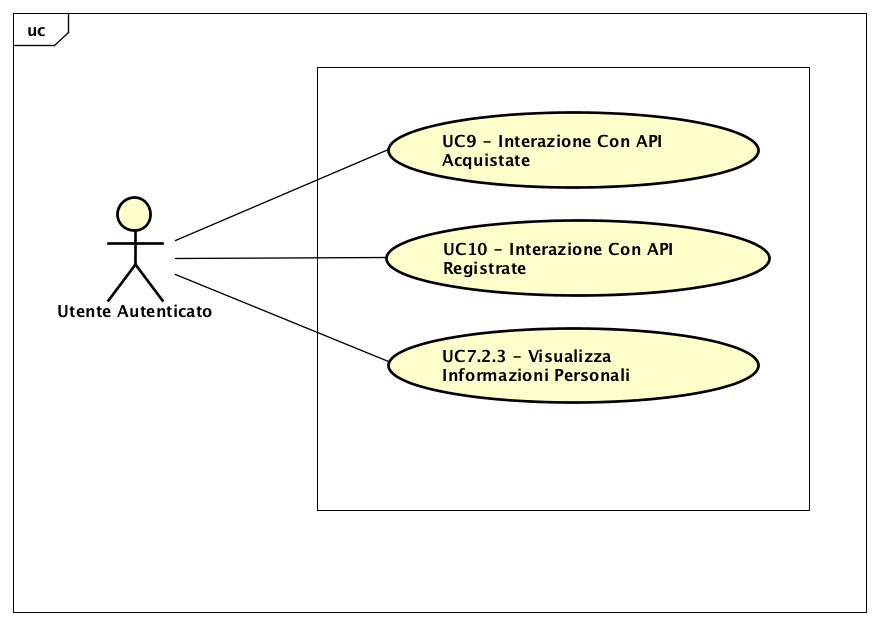
\includegraphics[scale=0.45]{UML/UC7_2.png}
	\caption{UC7.2 - Visualizzazione Proprio Profilo Utente}
\end{figure}
\FloatBarrier
\begin{longtable}{ l | p{11cm}}
	\hline
	\rowcolor{Gray}
	 \multicolumn{2}{c}{UC7.2 - Visualizzazione Proprio Profilo Utente} \\
	 \hline
	 \textbf{Attori} & Utente autenticato \\
	\textbf{Descrizione} & L’utente pu\'{o} visualizzare le proprie informazioni personali, interagire con le API da lui registrate e con le API acquistate  \\
	\textbf{Pre-Condizioni} & L’Utente \`{e} nel proprio profilo \\
	\textbf{Post-Condizioni} & L’Utente ha scelto l'interazione con il proprio profilo \\
	\textbf{Scenario Principale} & 
	\begin{enumerate*}[label=(\arabic*.),itemjoin={\newline}]
		\item L'utente pu\`{o} interagire con le API acquistate (UC9)
		\item L'utente pu\`{o} interagire con le API registrate (UC10)
		\item L'utente pu\`{o} visualizzare le Informazioni personali (UC7.2.3)
	\end{enumerate*}\\
\end{longtable}



%\paragraph{Caso d'uso UC7.2.3:  Visualizza Informazioni Personali}
\label{UC7_2_3}
\begin{figure}[ht]
	\centering
	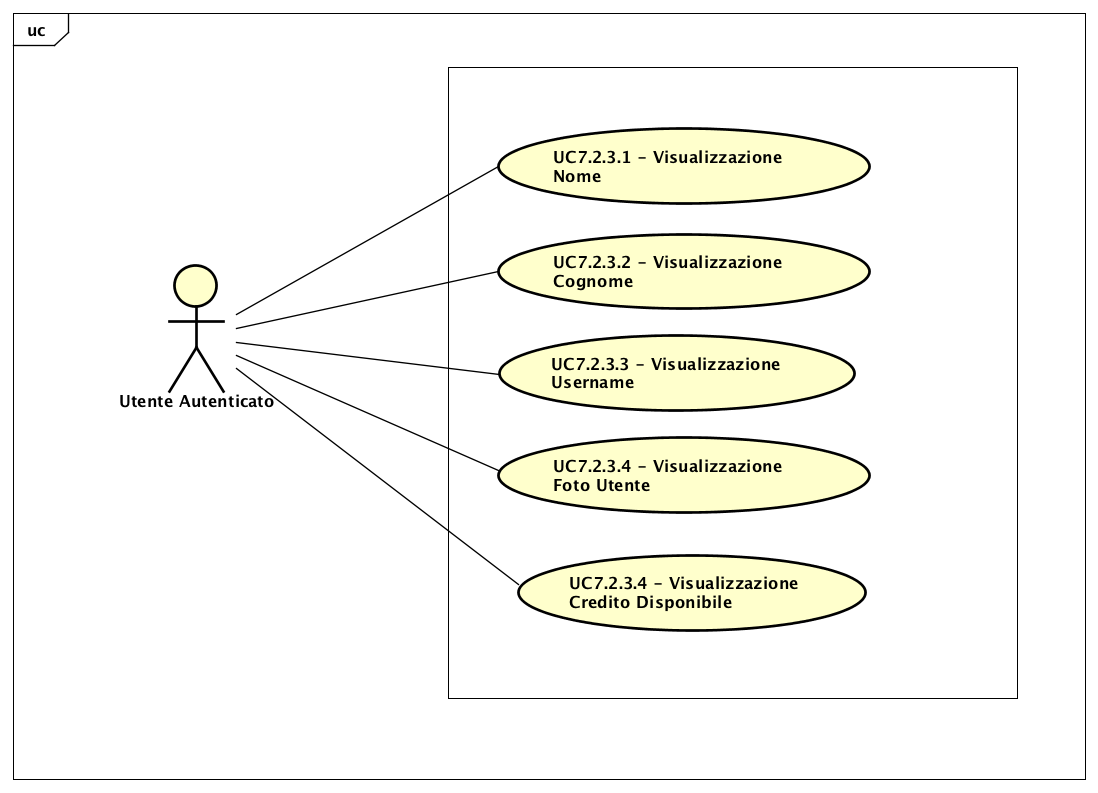
\includegraphics[scale=0.45]{UML/UC7_2_3.png}
	\caption{UC7.2.3: Visualizza Informazioni Personali}
\end{figure}

\FloatBarrier
\begin{tabular}{ l | p{11cm}}
	\hline
	\rowcolor{Gray}
	 \multicolumn{2}{c}{UC7.2.3:  VIsualizza Informazioni Personali} \\
	 \hline
	\textbf{Attori} & Utente Autenticato \\
	\textbf{Descrizione} & Gli utenti visualizzano le informazioni del proprio Profilo Utente\\
	\textbf{Pre-Condizioni} & L'utente e' nella schermata di gestione Profilo\\
	\textbf{Post-Condizioni} & L'utente ha modificato con successo il proprio Cognome \\
	\textbf{Scenario Principale} & 
	\begin{enumerate*}[label=(\arabic*.),itemjoin={\newline}]
		\item L'utente puo' Visualizzare il Nome (UC7.1.3.1)
		\item L'utente puo' Visualizzare il Cognome (UC7.1.3.2)
		\item L'utente puo' Visualizzare l'Username (UC7.1.3.3)
		\item L'utente puo' Visualizzare la Foto Utente (UC7.1.3.4)
		\item L'utente puo' Visualizzare il suo Credito Disponibile (UC7.1.3.4)
	\end{enumerate*}\\
\end{tabular}

%\newpage
\subsection{Caso d'uso UC8: Visualizzazione API acquistate}
\label{UC8}
\begin{figure}[ht]
	\centering
	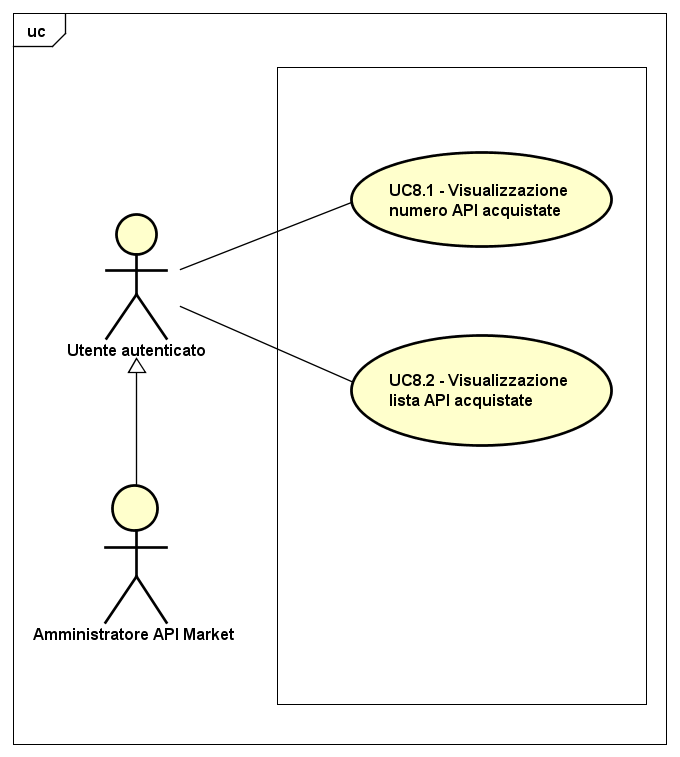
\includegraphics[scale=0.45]{UML/UC8.png}
	\caption{UC8: Visualizzazione API acquistate}
\end{figure}

\begin{longtable}{ l | p{11cm}}
	\hline
	\rowcolor{Gray}
	\multicolumn{2}{c}{UC8 - Visualizzazione API acquistate}\\
	\hline
	 \textbf{Attori} & Utente autenticato, Amministratore API Market \\
	\textbf{Descrizione} & L'attore visualizza le API da lui acquistate \\
	\textbf{Pre-Condizioni} & L'attore si trova nella schermata relativa alle API da lui acquistate \\
	\textbf{Post-Condizioni} & L'attore ha visualizzato le API da lui acquistate \\
	\textbf{Scenario Principale} & 
	\begin{enumerate*}[label=(\arabic*.),itemjoin={\newline}]
		\item L'attore può visualizzare il numero delle API acquistate e attive (UC8.1)
		\item L'attore può visualizzare la lista delle API acquistate e attive (UC8.2)
	\end{enumerate*}\\
\end{longtable}

\subsubsection{Caso d'uso UC8.1: Visualizzazione numero API acquistate}
\label{UC8_1}

\begin{minipage}{\linewidth}
	\begin{tabular}{ l | p{11cm}}
		\hline
		\rowcolor{Gray}
		\multicolumn{2}{c}{UC8.1 - Visualizzazione numero API acquistate} \\
		\hline
		\textbf{Attori} & Utente autenticato, Amministratore API Market \\
		\textbf{Descrizione} & L'attore visualizza il numero di API da lui acquistate \\
		\textbf{Pre-Condizioni} & L'attore si trova nella schermata relativa alle API da lui acquistate \\
		\textbf{Post-Condizioni} & L'attore ha visualizzato il numero delle API da lui acquistate \\
		\textbf{Scenario Principale} & 
		\begin{enumerate*}[label=(\arabic*.),itemjoin={\newline}]
			\item L'attore può visualizzare il numero di API acquistate
		\end{enumerate*}\\
	\end{tabular}
\end{minipage}

\newpage
\subsubsection{Caso d'uso UC8.2: Visualizzazione lista API acquistate}
\label{UC8_2}
\begin{figure}[ht]
	\centering
	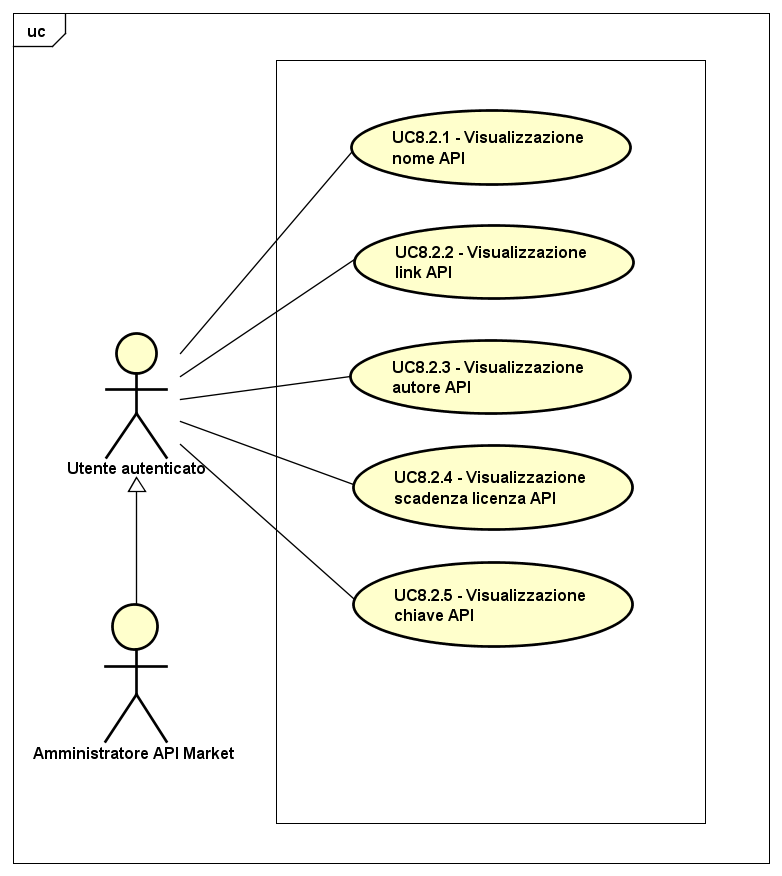
\includegraphics[scale=0.45]{UML/UC8_2.png}
	\caption{UC8.2: Visualizzazione lista API acquistate}
\end{figure}

\begin{minipage}{\linewidth}
	\begin{tabular}{ l | p{11cm}}
		\hline
		\rowcolor{Gray}
		\multicolumn{2}{c}{UC8.2 - Visualizzazione lista API acquistate} \\
		\hline
		\textbf{Attori} & Utente autenticato, Amministratore API Market \\
		\textbf{Descrizione} & L'attore visualizza la lista delle API da lui acquistate \\
		\textbf{Pre-Condizioni} & L'attore si trova nella schermata relativa alle API da lui acquistate \\
		\textbf{Post-Condizioni} & L'attore ha visualizzato la lista delle API da lui acquistate \\
		\textbf{Scenario Principale} & 
		\begin{enumerate*}[label=(\arabic*.),itemjoin={\newline}]
			\item L'attore può visualizzare il nome dell'API (UC8.2.1)
			\item L'attore può visualizzare il link alla pagina di visualizzazione API (UC8.2.2)
			\item L'attore può visualizzare il nome dell'autore dell'API (UC8.2.3)
			\item L'attore può visualizzare la policy divendita dell'API (UC8.2.4)
			\item L'attore può visualizzare il parametro di scadenza, in base al contratto,  della propria licenza per l'API (UC8.2.5)
			\item L'attore può visualizzare gli avvisi riguardo l'API (UC8.2.6)
		\end{enumerate*}\\
	\end{tabular}
\end{minipage}

\paragraph{Caso d'uso UC8.2.1: Visualizzazione nome API}
\label{UC8_2_1}

\begin{minipage}{\linewidth}
	\begin{tabular}{ l | p{11cm}}
		\hline
		\rowcolor{Gray}
		\multicolumn{2}{c}{UC8.2.1 - Visualizzazione nome API} \\
		\hline
		\textbf{Attori} & Utente autenticato, Amministratore API Market \\
		\textbf{Descrizione} & L'attore visualizza nella lista il nome dell'API \\
		\textbf{Pre-Condizioni} & L'attore si trova nella schermata relativa alle API da lui acquistate \\
		\textbf{Post-Condizioni} & L'attore ha visualizzato nella lista il nome dell'API \\
		\textbf{Scenario Principale} & 
		\begin{enumerate*}[label=(\arabic*.),itemjoin={\newline}]
			\item L'attore può visualizzare nella lista il nome dell'API
		\end{enumerate*}\\
	\end{tabular}
\end{minipage}

\paragraph{Caso d'uso UC8.2.2: Visualizzazione link API}
\label{UC8_2_2}

\begin{minipage}{\linewidth}
	\begin{tabular}{ l | p{11cm}}
		\hline
		\rowcolor{Gray}
		\multicolumn{2}{c}{UC8.2.2 - Visualizzazione link API} \\
		\hline
		\textbf{Attori} & Utente autenticato, Amministratore API Market \\
		\textbf{Descrizione} & L'attore visualizza nella lista il link alla visualizzazione dell'API \\
		\textbf{Pre-Condizioni} & L'attore si trova nella schermata di visualizzazione delle API acquistate \\
		\textbf{Post-Condizioni} & L'attore ha visualizzato nella lista il link alla visualizzazione dell'API \\
		\textbf{Scenario Principale} & 
		\begin{enumerate*}[label=(\arabic*.),itemjoin={\newline}]
			\item L'attore può visualizzare nella lista il link alla visualizzazione dell'API, che lo reindirizzerà ad UC7 per l'API in questione
		\end{enumerate*}\\
	\end{tabular}
\end{minipage}

\paragraph{Caso d'uso UC8.2.3: Visualizzazione nome autore API}
\label{UC8_2_3}

\begin{minipage}{\linewidth}
	\begin{tabular}{ l | p{11cm}}
		\hline
		\rowcolor{Gray}
		\multicolumn{2}{c}{UC8.2.3 - Visualizzazione nome autore API} \\
		\hline
		\textbf{Attori} & Utente autenticato, Amministratore API Market \\
		\textbf{Descrizione} & L'attore visualizza nella lista il nome dell'autore dell'API \\
		\textbf{Pre-Condizioni} & L'attore si trova nella schermata relativa alle API da lui acquistate \\
		\textbf{Post-Condizioni} & L'attore ha visualizzato nella lista il nome dell'autore dell'API \\
		\textbf{Scenario Principale} & 
		\begin{enumerate*}[label=(\arabic*.),itemjoin={\newline}]
			\item L'attore può visualizzare nella lista il nome dell'autore dell'API
		\end{enumerate*}\\
	\end{tabular}
\end{minipage}

\paragraph{Caso d'uso UC8.2.4: Visualizzazione policy vendita API}
\label{UC8_2_4}

\begin{minipage}{\linewidth}
	\begin{tabular}{ l | p{11cm}}
		\hline
		\rowcolor{Gray}
		\multicolumn{2}{c}{UC8.2.4 - Visualizzazione policy vendita API} \\
		\hline
		\textbf{Attori} & Utente autenticato, Amministratore API Market \\
		\textbf{Descrizione} & L'attore visualizza nella lista la policy di vendita dell'API \\
		\textbf{Pre-Condizioni} & L'attore si trova nella schermata relativa alle API da lui acquistate \\
		\textbf{Post-Condizioni} & L'attore ha visualizzato nella lista la policy di vendita dell'API \\
		\textbf{Scenario Principale} & 
		\begin{enumerate*}[label=(\arabic*.),itemjoin={\newline}]
			\item L'attore può visualizzare nella lista la policy di vendita dell'API
		\end{enumerate*}\\
	\end{tabular}
\end{minipage}

\paragraph{Caso d'uso UC8.2.5: Visualizzazione scadenza licenza}
\label{UC8_2_5}

\begin{minipage}{\linewidth}
	\begin{tabular}{ l | p{11cm}}
		\hline
		\rowcolor{Gray}
		\multicolumn{2}{c}{UC8.2.3 - Visualizzazione scadenza licenza} \\
		\hline
		\textbf{Attori} & Utente autenticato, Amministratore API Market \\
		\textbf{Descrizione} & L'attore visualizza nella lista la data di scadenza della propria licenza per l'API \\
		\textbf{Pre-Condizioni} & L'attore si trova nella schermata relativa alle API da lui acquistate \\
		\textbf{Post-Condizioni} & L'attore ha visualizzato nella lista il parametro di scadenza dell'API \\
		\textbf{Scenario Principale} & 
		\begin{enumerate*}[label=(\arabic*.),itemjoin={\newline}]
			\item L'attore può visualizzare nella lista il parametro di scadenza della propria licenza per l'API
		\end{enumerate*}\\
	\end{tabular}
\end{minipage}

\paragraph{Caso d'uso UC8.2.6: Avvisi API}
\label{UC8_2_6}

\begin{minipage}{\linewidth}
	\begin{tabular}{ l | p{11cm}}
		\hline
		\rowcolor{Gray}
		\multicolumn{2}{c}{UC8.2.6 - Avvisi API} \\
		\hline
		\textbf{Attori} & Utente autenticato, Amministratore API Market \\
		\textbf{Descrizione} & L'attore visualizza nella lista gli avvisi riguardanti l'API \\
		\textbf{Pre-Condizioni} & L'attore si trova nella schermata relativa alle API da lui acquistate \\
		\textbf{Post-Condizioni} & L'attore ha visualizzato nella lista gli avvisi riguardanti l'API \\
		\textbf{Scenario Principale} & 
		\begin{enumerate*}[label=(\arabic*.),itemjoin={\newline}]
			\item L'attore può visualizzare nella lista gli avvisi riguardanti l'API (E.g: cancellazione, manutenzione)
		\end{enumerate*}\\
	\end{tabular}
\end{minipage}
%\subsubsection{Caso d'uso UC8.1 - Consultazione Documentazione API}
\label{UC8.1}
\begin{figure}[ht]
	\centering
	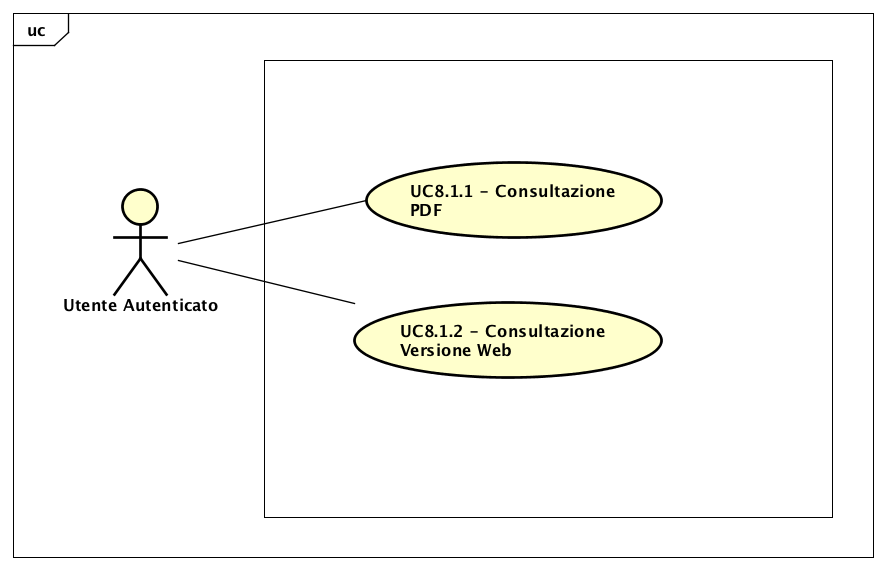
\includegraphics[scale=0.45]{UML/UC8_1.png}
	\caption{UC8.1 - Consultazione Documentazione API}
\end{figure}
\FloatBarrier
\begin{longtable}{ l | p{11cm}}
	\hline
	\rowcolor{Gray}
	\multicolumn{2}{c}{UC8.1 - Consultazione Documentazione API}\\
	\hline
	
	 \textbf{Attori} & Utente autenticato  \\
	\textbf{Descrizione} & L'utente puo' consultare la Documentazione delle API \\
	\textbf{Pre-Condizioni} & L'utente e' autenticato in APIMarket e ha scelto una API dalla lista API\\
	\textbf{Post-Condizioni} & L'utente ha visualizzato la documetazione e ora puo' scegliere un'altra interazione\\
	\textbf{Scenario Principale} & 
	\begin{enumerate*}[label=(\arabic*.),itemjoin={\newline}]
		\item L'utente puo' Consultare la versione PDF della Documentazione (UC8.1.1)
		\item L'utente puo' Consultare la versione Web della Documentazione (UC8.1.2)
	\end{enumerate*}\\
\end{longtable}


%\paragraph{Caso d'uso UC8.1.1: Consultazione PDF}
\label{UC8.1.1}

\renewcommand*{\arraystretch}{1.6}
\begin{longtable}{ l | p{11cm}}
	\hline
	\rowcolor{Gray}
	\multicolumn{2}{c}{UC8.1.1: Consultazione PDF} \\
	\hline
	\textbf{Attori} &Utente Autenticato, Amministratore APIMarket \\
	\textbf{Descrizione} & l'attore visualizza la documentazione dell'API \\
	\textbf{Pre-Condizioni} &  l'attore ha scelto di consultare la documentazione di un'API\\
	\textbf{Post-Condizioni}& l'attore vede il PDF della documentazione\\
	\textbf{Scenario Principale} & \begin{enumerate*}[label=(\arabic*.),itemjoin={\newline}]
		\item L'attore vede la documentazione in PDF
	\end{enumerate*}\\
\end{longtable}

%\newpage
\paragraph{Caso d'uso UC8.1.2: Consultazione Versione Web}
\label{UC8.1.2}

\renewcommand*{\arraystretch}{1.6}
\begin{longtable}{ l | p{11cm}}
	\hline
	\rowcolor{Gray}
	\multicolumn{2}{c}{UC8.1.2: Consultazione Versione Web} \\
	\hline
	\textbf{Attori} &Utente Autenticato, Amministratore APIMarket \\
	\textbf{Descrizione} & l'attore visualizza la documentazione dell'API \\
	\textbf{Pre-Condizioni} &  l'attore ha scelto di consultare la documentazione di un'API\\
	\textbf{Post-Condizioni}& l'attore vede la versione Web della documentazione\\
	\textbf{Scenario Principale} & \begin{enumerate*}[label=(\arabic*.),itemjoin={\newline}]
		\item L'attore vede la documentazione in versione Web
	\end{enumerate*}\\
\end{longtable}

%
\subsubsection{Caso d'uso UC8.2 - Procedura di Acquisto API}
\label{UC8.2}
\begin{figure}[ht]
	\centering
	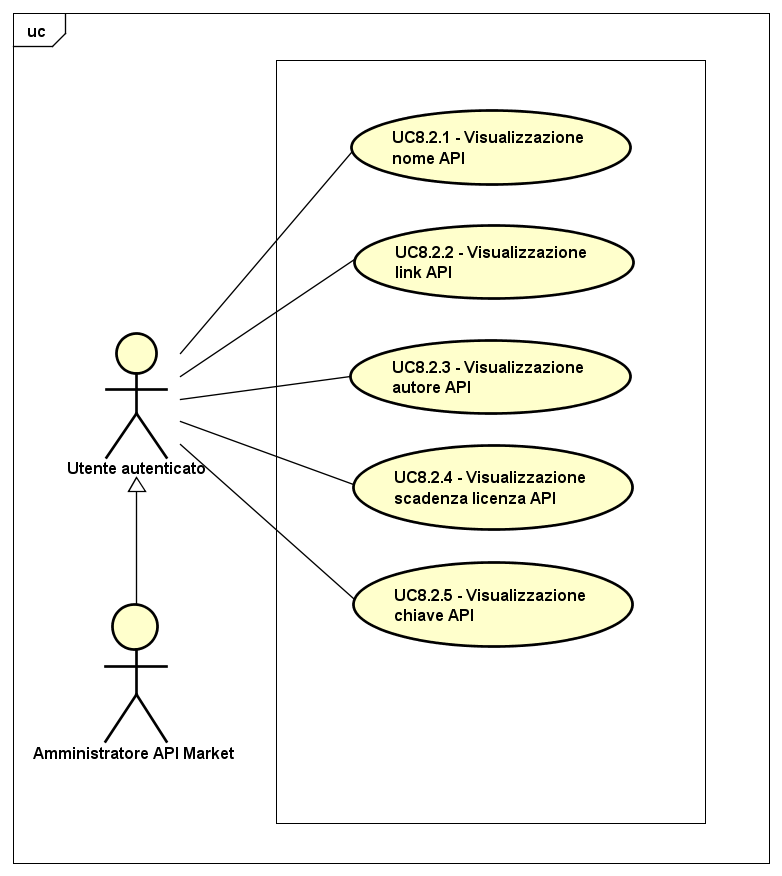
\includegraphics[scale=0.45]{UML/UC8_2.png}
	\caption{UC8.2 - Procedura di Acquisto API}
\end{figure}
\FloatBarrier
\begin{longtable}{ l | p{11cm}}
	\hline
	\rowcolor{Gray}
	\multicolumn{2}{c}{UC8.2 - Procedura di Acquisto API}\\
	\hline
	 \textbf{Attori} & Utente autenticat, Amministratore APIMarket, Sistema \\
	\textbf{Descrizione} & L'utente puo' comprare un'API e puo' farlo in diversi modi, anche secondo una procedura esterna (un esempio di procedura esterna e' Paypal)\\
	\textbf{Pre-Condizioni} & L'utente ha selezionato un'API\\
	\textbf{Post-Condizioni} & L'utente ha acquistato l'API e ricevuto la chiave API associata\\
	\textbf{Scenario Principale} & 
	\begin{enumerate*}[label=(\arabic*.),itemjoin={\newline}]
		\item L'utente puo' scegliere il Piano di Acquisto(UC8.2.1)
		\item L'utente puo' scegliere la modalita' di Acquisto (UC8.2.2)
		\item L'utente puo' confermare l'Acquisto (UC8.2.3)
		\item L'utente puo' Visualizzare l'Errore di Acquisto (UC8.2.4)
		\item L'utente puo' confermare l'Acquisto Avvenuto (UC8.2.5)
		\item Il sistema puo' eseguire l'Acquisto usando una procedura d'Acquisto esterna (UC8.2.6)
		\item L'utente puo' ricevere una Chiave API dopo l'Acquisto (UC8.2.7)
	\end{enumerate*}\\
	\textbf{Scenari Alternativi} & 
	\begin{enumerate*}[label=(\arabic*.),itemjoin={\newline}]
		\item L'utente puo' Visualizzare l'Errore di Acquisto (UC8.2.4)
	\end{enumerate*}\\
\end{longtable}

%\paragraph{Caso d'uso UC8.2.1: Scelta Piano di Acquisto}
\label{UC8.2.1}

\renewcommand*{\arraystretch}{1.6}
\begin{longtable}{ l | p{11cm}}
	\hline
	\rowcolor{Gray}
	\multicolumn{2}{c}{UC8.2.1: Scelta Piano di Acquisto} \\
	\hline
	\textbf{Attori} &Utente Autenticato, Amministratore APIMarket\\
	\textbf{Descrizione} & ll'Attore deve scelgliere un Piano d'Acquisto da un insieme di Piani d'Acquisto\\
	\textbf{Pre-Condizioni} &  L'attore ha avviato la procedura di Acquisto\\
	\textbf{Post-Condizioni}& L'attore ha scelto un piano di Acquisto\\
	\textbf{Scenario Principale} & \begin{enumerate*}[label=(\arabic*.),itemjoin={\newline}]
		\item L'attore ha una lista di Piani D'Acquisto e ne sceglie uno
	\end{enumerate*}\\
\end{longtable}

%\paragraph{Caso d'uso UC8.2.2: Scelta' Modalita' di Acquisto}
\label{UC8.2.2}

\renewcommand*{\arraystretch}{1.6}
\begin{longtable}{ l | p{11cm}}
	\hline
	\rowcolor{Gray}
	\multicolumn{2}{c}{UC8.2.2: Scelta' Modalita' di Acquisto} \\
	\hline
	\textbf{Attori} &Utente Autenticato, Amministratore APIMarket, Interfacce API Presente In APIMarket \\
	\textbf{Descrizione} & l'attore visualizza un insieme di modalita' di acquisto (es. Paypal, carta) e sceglie quella che preferisce\\
	\textbf{Pre-Condizioni} & L'attore e' nel processo di Acquisto di una API\\
	\textbf{Post-Condizioni}& L'attore ha scelto la sua modalita' di Acquisto\\
	\textbf{Scenario Principale} & \begin{enumerate*}[label=(\arabic*.),itemjoin={\newline}]
		\item L'attore sceglie la modalita' di acquisto
	\end{enumerate*}\\
\end{longtable}

%\paragraph{Caso d'uso UC8.2.3: Conferma Acquisto}
\label{UC8.2.3}

\renewcommand*{\arraystretch}{1.6}
\begin{longtable}{ l | p{11cm}}
	\hline
	\rowcolor{Gray}
	\multicolumn{2}{c}{UC8.2.3: Conferma Acquisto} \\
	\hline
	\textbf{Attori} &Utente Autenticato, Amministratore APIMarket \\
	\textbf{Descrizione} & l'attore sceglie conferma l'acquisto e il processo di pagamento puo' avvenire\\
	\textbf{Pre-Condizioni} &  l'attore ha scelto di acquistare una API e scelto le modalita' di acquisto\\
	\textbf{Post-Condizioni}& l'attore ha pagato e acquistato la API\\
	\textbf{Scenario Principale} & \begin{enumerate*}[label=(\arabic*.),itemjoin={\newline}]
		\item L'attore conferma l'acquisto
	\end{enumerate*}\\
\end{longtable}

%\paragraph{Caso d'uso UC8.2.4: Visualizzazione Errore Acquisto}
\label{UC8.2.4}

\renewcommand*{\arraystretch}{1.6}
\begin{longtable}{ l | p{11cm}}
	\hline
	\rowcolor{Gray}
	\multicolumn{2}{c}{UC8.2.4: Visualizzazione Errore Acquisto} \\
	\hline
	\textbf{Attori} &Utente Autenticato, Amministratore APIMarket\\
	\textbf{Descrizione} & L'attore ha provato a effettuare l'acquisto ma i dati inseriti sono errati\\
	\textbf{Pre-Condizioni} &  l'attore ha confermato l'acquisto\\
	\textbf{Post-Condizioni}& l'attore deve reinserire le informazioni d'Acquisto\\
	\textbf{Scenario Principale} & \begin{enumerate*}[label=(\arabic*.),itemjoin={\newline}]
		\item L'attore visualizza l'Errore d'Acquisto
	\end{enumerate*}\\
	\textbf{Scenari Alternativi} & \begin{enumerate*}[label=(\arabic*.),itemjoin={\newline}]
		\item L'attore sceglie di annullare l'Acquisto
	\end{enumerate*}\\
\end{longtable}

%\paragraph{Caso d'uso UC8.2.5: Conferma Acquisto Avvenuto}
\label{UC8.2.5}

\renewcommand*{\arraystretch}{1.6}
\begin{longtable}{ l | p{11cm}}
	\hline
	\rowcolor{Gray}
	\multicolumn{2}{c}{UC8.2.5: Conferma Acquisto Avvenuto} \\
	\hline
	\textbf{Attori} &Utente Autenticato, Amministratore APIMarket \\
	\textbf{Descrizione} & l'attore riceve una conferma dal sistema che segnala il successo dell'Acquisto  \\
	\textbf{Pre-Condizioni} &  l'attore ha confermato l'acquisto\\
	\textbf{Post-Condizioni}& l'attore riceve la chiave dell'API\\
	\textbf{Scenario Principale} & \begin{enumerate*}[label=(\arabic*.),itemjoin={\newline}]
		\item L'attore visualizza una conferma che segnala un Acquisto di successo
	\end{enumerate*}\\
\end{longtable}

%\paragraph{Caso d'uso UC8.2.6: Procedura Acquisto Esterna}
\label{UC8.2.6}

\renewcommand*{\arraystretch}{1.6}
\begin{longtable}{ l | p{11cm}}
	\hline
	\rowcolor{Gray}
	\multicolumn{2}{c}{UC8.2.6: Procedura Acquisto Esterna} \\
	\hline
	\textbf{Attori} &Utente Autenticato, Amministratore APIMarket\\
	\textbf{Descrizione} & l'attore usa una procedura d'acquisto esterna per acquistare l'API \\
	\textbf{Pre-Condizioni} &  l'attore ha confermato l'acquisto\\
	\textbf{Post-Condizioni}& l'attore ha pagato l'API e riceve la chiave API\\
	\textbf{Scenario Principale} & \begin{enumerate*}[label=(\arabic*.),itemjoin={\newline}]
		\item L'attore può pagare usando una procedura d'acquisto esterna
	\end{enumerate*}\\
\end{longtable}

%\paragraph{Caso d'uso UC8.2.7: Rilascio Chiave API}
\label{UC8.2.7}

\renewcommand*{\arraystretch}{1.6}
\begin{longtable}{ l | p{11cm}}
	\hline
	\rowcolor{Gray}
	\multicolumn{2}{c}{UC8.2.7: Rilascio Chiave API} \\
	\hline
	\textbf{Attori} &Utente Autenticato, Amministratore APIMarket \\
	\textbf{Descrizione} & l'attore riceve una chiave API e puo' iniziare a usare l'API \\
	\textbf{Pre-Condizioni} &  l'attore ha comprato l'API\\
	\textbf{Post-Condizioni}& l'attore ha la chiave API e puo' usarla fino alla scadenza della chiave\\
	\textbf{Scenario Principale} & \begin{enumerate*}[label=(\arabic*.),itemjoin={\newline}]
		\item L'attore riceve una chiave API valida fino a una certa data o fino al rinnovo
	\end{enumerate*}\\
\end{longtable}

%\newpage
\subsection{Caso d'uso UC9: Acquisto API}
\label{UC9}
\begin{figure}[ht]
	\centering
	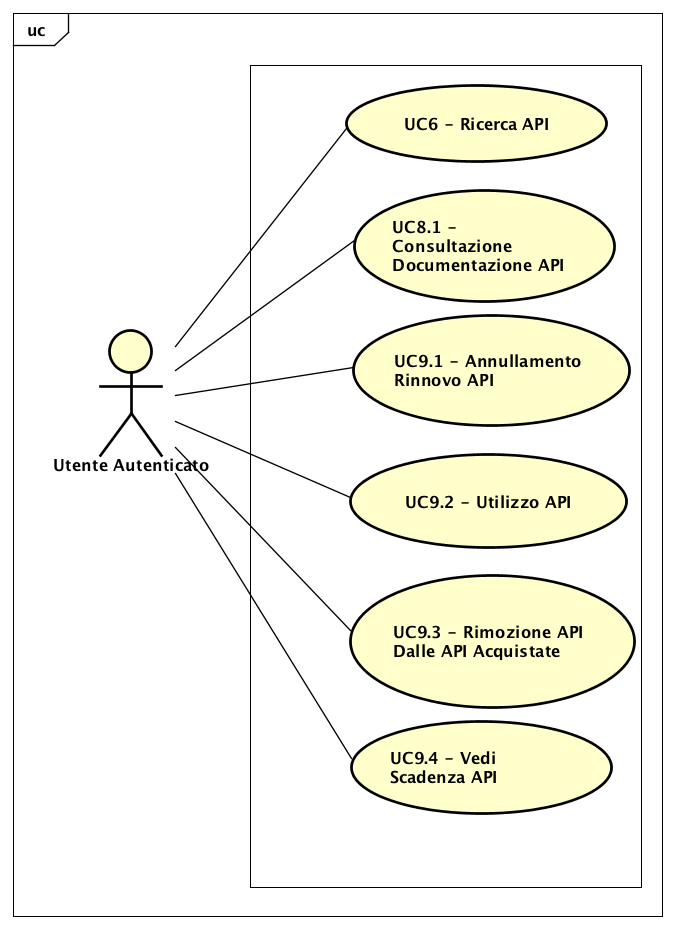
\includegraphics[scale=0.45]{UML/UC9.png}
	\caption{UC9: Acquisto API}
\end{figure}

\begin{longtable}{ l | p{11cm}}
	\hline
	\rowcolor{Gray}
	\multicolumn{2}{c}{UC9 - Acquisto API}\\
	\hline
	\textbf{Attori} & Utente autenticato, Amministratore API Market \\
	\textbf{Descrizione} & L'attore può effettuare l'acquisto dell'API selezionata tramite i crediti da lui posseduti \\
	\textbf{Pre-Condizioni} & L'attore ha selezionato una API e si trova nella relativa schermata di acquisto \\
	\textbf{Post-Condizioni} & L'attore ha acquistato l'API selezionata \\
	\textbf{Scenario Principale} & 
	\begin{enumerate*}[label=(\arabic*.),itemjoin={\newline}]
		\item L'attore può visualizzare il nome dell'API (UC9.1)
		\item L'attore può visualizzare l'autore dell'API (UC9.2)
		\item L'attore può scegliere la licenza API desiderata (UC9.3)
		\item L'attore può visualizzare il prezzo dell'API selezionata (UC9.4)
		\item L'attore può visualizzare il saldo disponibile nel suo conto virtuale (UC12.2.1)
		\item L'attore può ricaricare il proprio conto virtuale (UC12.2.2)
		\item L'attore può visualizzare il saldo preventivato in seguito all'acquisto della licenza selezionata (UC9.5)
		\item L'attore può confermare l'acquisto (UC9.6), venendo reindirizzato ad una schermata di riepilogo (UC9.7)
	\end{enumerate*}\\
	\textbf{Scenari Alternativi} & 
	\begin{enumerate*}[label=(\arabic*.),itemjoin={\newline}]
		\item L'attore può visualizzare un messaggio di errore e la transazione non avviene (UC9.8)
	\end{enumerate*}\\
\end{longtable}

\subsubsection{Caso d'uso UC9.1: Visualizzazione nome API}
\label{UC9_1}

\begin{minipage}{\linewidth}
	\begin{tabular}{ l | p{11cm}}
		\hline
		\rowcolor{Gray}
		\multicolumn{2}{c}{UC9.1 - Visualizzazione nome API} \\
		\hline
		\textbf{Attori} & Utente autenticato, Amministratore API Market \\
		\textbf{Descrizione} & L'attore visualizza il nome dell'API \\
		\textbf{Pre-Condizioni} & L'attore si trova nella schermata di acquisto dell'API \\
		\textbf{Post-Condizioni} & L'attore ha visualizzato il nome dell'API \\
		\textbf{Scenario Principale} & 
		\begin{enumerate*}[label=(\arabic*.),itemjoin={\newline}]
			\item L'attore può visualizzare il nome dell'API
		\end{enumerate*}\\
	\end{tabular}
\end{minipage}

\subsubsection{Caso d'uso UC9.2: Visualizzazione nome API}
\label{UC9_2}

\begin{minipage}{\linewidth}
	\begin{tabular}{ l | p{11cm}}
		\hline
		\rowcolor{Gray}
		\multicolumn{2}{c}{UC9.2 - Visualizzazione autore API} \\
		\hline
		\textbf{Attori} & Utente autenticato, Amministratore API Market \\
		\textbf{Descrizione} & L'attore visualizza l'autore dell'API \\
		\textbf{Pre-Condizioni} & L'attore si trova nella schermata di acquisto dell'API \\
		\textbf{Post-Condizioni} & L'attore ha visualizzato l'autore dell'API \\
		\textbf{Scenario Principale} & 
		\begin{enumerate*}[label=(\arabic*.),itemjoin={\newline}]
			\item L'attore può visualizzare l'autore dell'API
		\end{enumerate*}\\
	\end{tabular}
\end{minipage}

\newpage
\subsubsection{Caso d'uso UC9.3: Scelta licenza API}
\label{UC9_3}
\begin{figure}[ht]
	\centering
	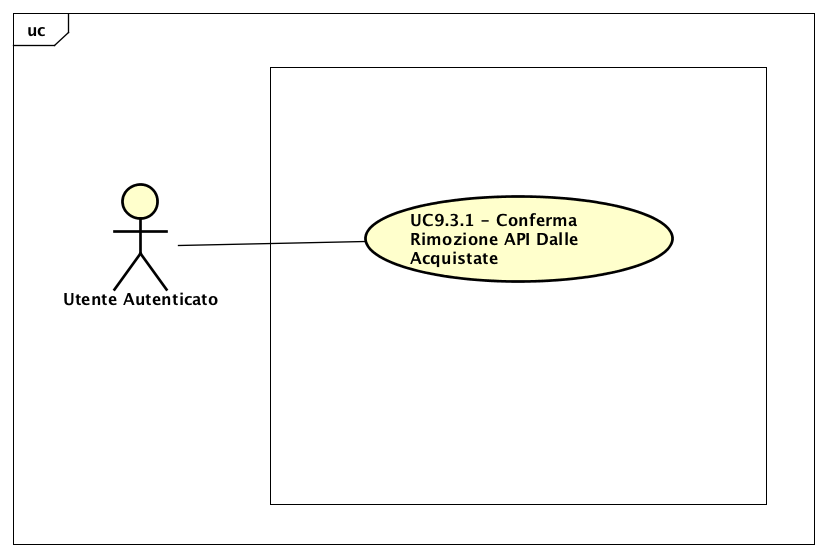
\includegraphics[scale=0.45]{UML/UC9_3.png}
	\caption{UC9.3: Scelta licenza API}
\end{figure}

\begin{minipage}{\linewidth}
	\begin{tabular}{ l | p{11cm}}
		\hline
		\rowcolor{Gray}
		\multicolumn{2}{c}{UC9.1 - Visualizzazione menù licenza} \\
		\hline
		\textbf{Attori} & Utente autenticato, Amministratore API Market \\
		\textbf{Descrizione} & L'attore sceglie tra le licenze quella desiderata, oppure lascia inalterata la scelta di default \\
		\textbf{Pre-Condizioni} & L'attore ha selezionato una API e si trova nella relativa schermata di acquisto \\
		\textbf{Post-Condizioni} & L'attore ha selezionato la licenza desiderata, oppure ha lasciato inalterata la scelta di default \\
		\textbf{Scenario Principale} & 
		\begin{enumerate*}[label=(\arabic*.),itemjoin={\newline}]
			\item L'attore può selezionare la licenza per numero di chiamate, impostata di default (UC9.3.1)
			\item L'attore può selezionare la licenza per tempo di utilizzo (UC9.3.2)
			\item L'attore può selezionare la licenza per traffico (UC9.3.3)
		\end{enumerate*}\\
	\end{tabular}
\end{minipage}

\paragraph{Caso d'uso UC9.3.1: Scelta licenza per numero di chiamate}
\label{UC9_3_1}

\begin{minipage}{\linewidth}
	\begin{tabular}{ l | p{11cm}}
		\hline
		\rowcolor{Gray}
		\multicolumn{2}{c}{UC9.3.1 - Scelta licenza per numero di chiamate} \\
		\hline
		\textbf{Attori} & Utente autenticato, Amministratore API Market \\
		\textbf{Descrizione} & L'attore sceglie la licenza API per numero di chiamate \\
		\textbf{Pre-Condizioni} & L'attore si trova nella schermata di acquisto dell'API \\
		\textbf{Post-Condizioni} & L'attore ha scelto la licenza API per numero di chiamate \\
		\textbf{Scenario Principale} & 
		\begin{enumerate*}[label=(\arabic*.),itemjoin={\newline}]
			\item L'attore può scegliere la licenza API per numero di chiamate
		\end{enumerate*}\\
	\end{tabular}
\end{minipage}

\paragraph{Caso d'uso UC9.3.2: Scelta licenza per tempo di utilizzo}
\label{UC9_3_2}

\begin{minipage}{\linewidth}
	\begin{tabular}{ l | p{11cm}}
		\hline
		\rowcolor{Gray}
		\multicolumn{2}{c}{UC9.3.2 - Scelta licenza per tempo di utilizzo} \\
		\hline
		\textbf{Attori} & Utente autenticato, Amministratore API Market \\
		\textbf{Descrizione} & L'attore sceglie la licenza API per tempo di utilizzo \\
		\textbf{Pre-Condizioni} & L'attore si trova nella schermata di acquisto dell'API \\
		\textbf{Post-Condizioni} & L'attore ha scelto la licenza API per tempo di utilizzo \\
		\textbf{Scenario Principale} & 
		\begin{enumerate*}[label=(\arabic*.),itemjoin={\newline}]
			\item L'attore può scegliere la licenza API per tempo di utilizzo
		\end{enumerate*}\\
	\end{tabular}
\end{minipage}

\paragraph{Caso d'uso UC9.3.3: Scelta licenza per traffico}
\label{UC9_3_3}

\begin{minipage}{\linewidth}
	\begin{tabular}{ l | p{11cm}}
		\hline
		\rowcolor{Gray}
		\multicolumn{2}{c}{UC9.3.3 - Scelta licenza per traffico} \\
		\hline
		\textbf{Attori} & Utente autenticato, Amministratore API Market \\
		\textbf{Descrizione} & L'attore sceglie la licenza API per traffico \\
		\textbf{Pre-Condizioni} & L'attore si trova nella schermata di acquisto dell'API \\
		\textbf{Post-Condizioni} & L'attore ha scelto la licenza API per traffico \\
		\textbf{Scenario Principale} & 
		\begin{enumerate*}[label=(\arabic*.),itemjoin={\newline}]
			\item L'attore può scegliere la licenza API per traffico
		\end{enumerate*}\\
	\end{tabular}
\end{minipage}

\newpage
\subsubsection{Caso d'uso UC9.4: Visualizzazione prezzo API}
\label{UC9_4}
\begin{figure}[ht]
	\centering
	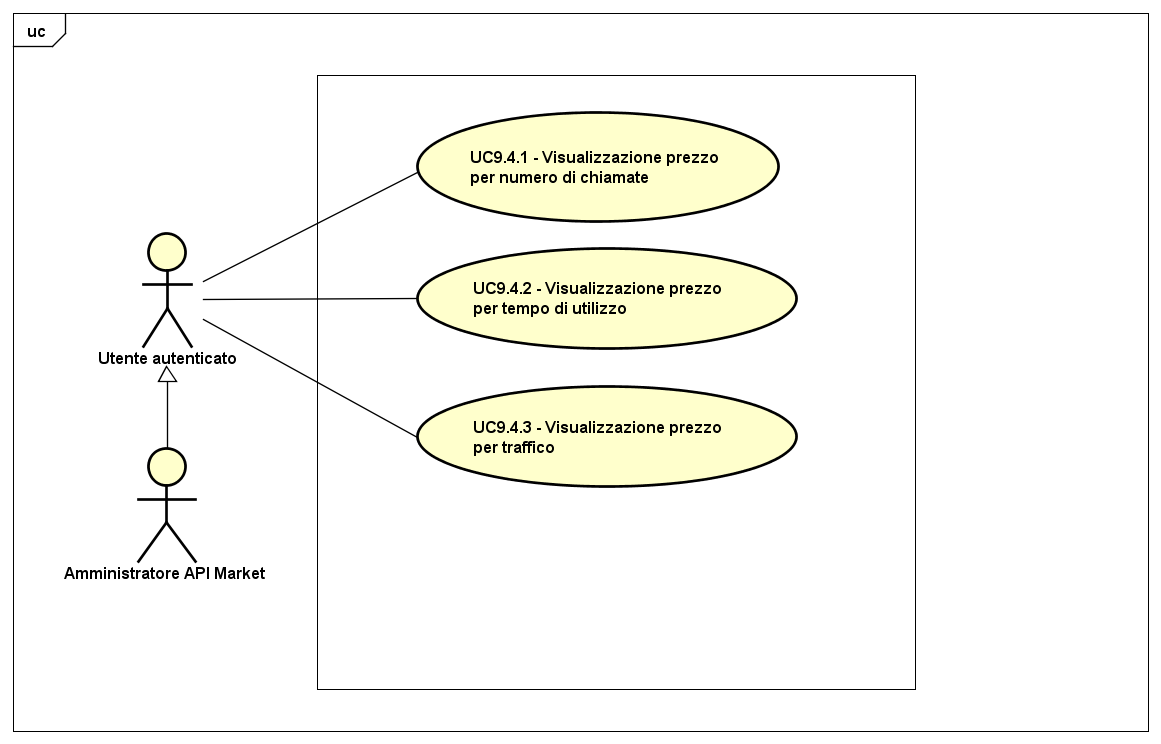
\includegraphics[scale=0.45]{UML/UC9_4.png}
	\caption{UC9.4: Visualizzazione prezzo API}
\end{figure}

\begin{minipage}{\linewidth}
	\begin{tabular}{ l | p{11cm}}
		\hline
		\rowcolor{Gray}
		\multicolumn{2}{c}{UC9.4 - Visualizzazione prezzo API} \\
		\hline
		\textbf{Attori} & Utente autenticato, Amministratore API Market \\
		\textbf{Descrizione} & L'attore visualizza il prezzo dell'API \\
		\textbf{Pre-Condizioni} & L'attore si trova nella schermata di acquisto dell'API \\
		\textbf{Post-Condizioni} & L'attore ha visualizzato il prezzo dell'API \\
		\textbf{Scenario Principale} & 
		\begin{enumerate*}[label=(\arabic*.),itemjoin={\newline}]
			\item L'attore può visualizzare il prezzo dell'API per numero di chiamate (UC9.4.1)
			\item L'attore può visualizzare il prezzo dell'API per tempo di utilizzo (UC9.4.2)
			\item L'attore può visualizzare il prezzo dell'API per traffico (UC9.4.3)
		\end{enumerate*}\\
	\end{tabular}
\end{minipage}

\paragraph{Caso d'uso UC9.4.1: Visualizzazione prezzo per numero di chiamate}
\label{UC9_4_1}

\begin{minipage}{\linewidth}
	\begin{tabular}{ l | p{11cm}}
		\hline
		\rowcolor{Gray}
		\multicolumn{2}{c}{UC9.4.1 - Visualizzazione prezzo per numero di chiamate} \\
		\hline
		\textbf{Attori} & Utente autenticato, Amministratore API Market \\
		\textbf{Descrizione} & L'attore visualizza il prezzo per numero di chiamate dell'API \\
		\textbf{Pre-Condizioni} & L'attore si trova nella schermata di acquisto dell'API \\
		\textbf{Post-Condizioni} & L'attore ha visualizzato il prezzo per numero di chiamate dell'API \\
		\textbf{Scenario Principale} & 
		\begin{enumerate*}[label=(\arabic*.),itemjoin={\newline}]
			\item L'attore può visualizzare il prezzo per numero di chiamate dell'API
		\end{enumerate*}\\
	\end{tabular}
\end{minipage}

\paragraph{Caso d'uso UC9.4.2: Visualizzazione prezzo per tempo di utilizzo}
\label{UC9_4_2}

\begin{minipage}{\linewidth}
	\begin{tabular}{ l | p{11cm}}
		\hline
		\rowcolor{Gray}
		\multicolumn{2}{c}{UC9.4.2 - Visualizzazione prezzo per tempo di utilizzo} \\
		\hline
		\textbf{Attori} & Utente autenticato, Amministratore API Market \\
		\textbf{Descrizione} & L'attore visualizza il prezzo per tempo di utilizzo dell'API \\
		\textbf{Pre-Condizioni} & L'attore si trova nella schermata di acquisto dell'API \\
		\textbf{Post-Condizioni} & L'attore ha visualizzato il prezzo per tempo di utilizzo dell'API \\
		\textbf{Scenario Principale} & 
		\begin{enumerate*}[label=(\arabic*.),itemjoin={\newline}]
			\item L'attore può visualizzare il prezzo per tempo di utilizzo dell'API
		\end{enumerate*}\\
	\end{tabular}
\end{minipage}

\paragraph{Caso d'uso UC9.4.3: Visualizzazione prezzo per traffico}
\label{UC9_4_3}

\begin{minipage}{\linewidth}
	\begin{tabular}{ l | p{11cm}}
		\hline
		\rowcolor{Gray}
		\multicolumn{2}{c}{UC9.4.3 - Visualizzazione prezzo per traffico} \\
		\hline
		\textbf{Attori} & Utente autenticato, Amministratore API Market \\
		\textbf{Descrizione} & L'attore visualizza il prezzo per per traffico dell'API \\
		\textbf{Pre-Condizioni} & L'attore si trova nella schermata di acquisto dell'API \\
		\textbf{Post-Condizioni} & L'attore ha visualizzato il prezzo per per traffico dell'API \\
		\textbf{Scenario Principale} & 
		\begin{enumerate*}[label=(\arabic*.),itemjoin={\newline}]
			\item L'attore può visualizzare il prezzo per per traffico dell'API
		\end{enumerate*}\\
	\end{tabular}
\end{minipage}

\subsubsection{Caso d'uso UC9.5: Visualizzazione previsione saldo finale}
\label{UC9_5}

\begin{minipage}{\linewidth}
	\begin{tabular}{ l | p{11cm}}
		\hline
		\rowcolor{Gray}
		\multicolumn{2}{c}{UC9.5 - Visualizzazione previsione saldo finale} \\
		\hline
		\textbf{Attori} & Utente autenticato, Amministratore API Market \\
		\textbf{Descrizione} & L'attore visualizza una previsione del proprio saldo crediti in seguito all'acquisto\\
		\textbf{Pre-Condizioni} & L'attore ha selezionato una API e si trova nella relativa schermata di acquisto \\
		\textbf{Post-Condizioni} & L'attore ha visualizzato una previsione del proprio saldo in seguito all'acquisto \\
		\textbf{Scenario Principale} & 
		\begin{enumerate*}[label=(\arabic*.),itemjoin={\newline}]
			\item L'attore può visualizzare una previsione del proprio saldo finale qualora acquistasse l'API con la licenza scelta in UC9.3
		\end{enumerate*}\\
	\end{tabular}
\end{minipage}

\subsubsection{Caso d'uso UC9.6: Conferma acquisto API}
\label{UC9_6}

\begin{minipage}{\linewidth}
	\begin{tabular}{ l | p{11cm}}
		\hline
		\rowcolor{Gray}
		\multicolumn{2}{c}{UC9.6 - Conferma acquisto API} \\
		\hline
		\textbf{Attori} & Utente autenticato, Amministratore API Market \\
		\textbf{Descrizione} & L'attore può confermare l'acquisto dell'API, portando a termine la transazione, ricevendo un'email di riepilogo e visualizzando una schermata di riepilogo dell'acquisto appena realizzato \\
		\textbf{Pre-Condizioni} & L'attore ha selezionato una API e si trova nella relativa schermata di acquisto \\
		\textbf{Post-Condizioni} & L'attore ha confermato l'acquisto dell'API \\
		\textbf{Scenario Principale} & 
		\begin{enumerate*}[label=(\arabic*.),itemjoin={\newline}]
			\item L'attore può confermare l'acquisto dell'API, portando a termine la transazione, ricevendo un'email di riepilogo e visualizzando una schermata di riepilogo dell'acquisto appena realizzato (UC9.7)
		\end{enumerate*}\\
	\end{tabular}
\end{minipage}

\newpage
\subsubsection{Caso d'uso UC9.7: Riepilogo acquisto API}
\label{UC9_7}
\begin{figure}[ht]
	\centering
	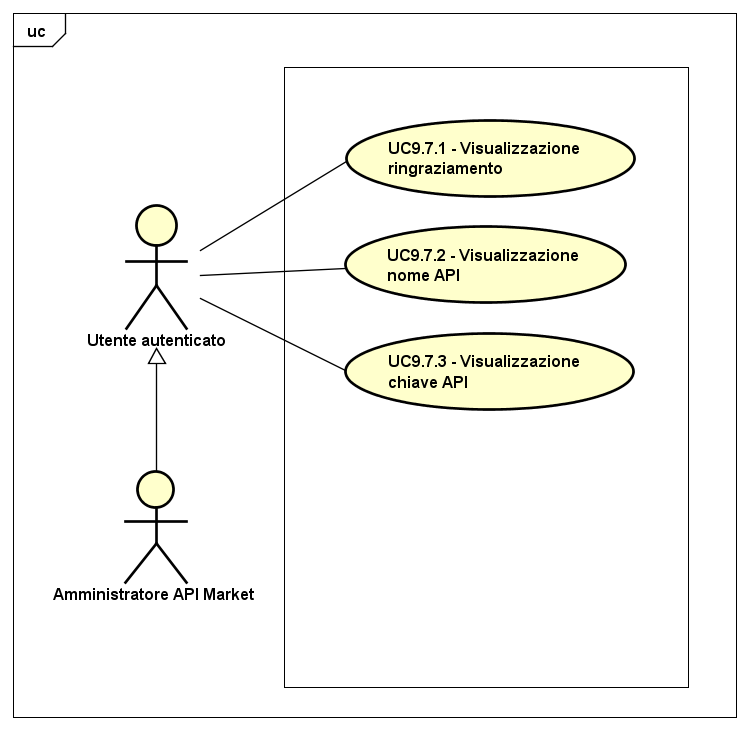
\includegraphics[scale=0.45]{UML/UC9_7.png}
	\caption{UC9.7: Riepilogo acquisto API}
\end{figure}

\begin{minipage}{\linewidth}
	\begin{tabular}{ l | p{11cm}}
		\hline
		\rowcolor{Gray}
		\multicolumn{2}{c}{UC9.7 - Riepilogo acquisto API} \\
		\hline
		\textbf{Attori} & Utente autenticato, Amministratore API Market \\
		\textbf{Descrizione} & L'attore conferma l'acquisto dell'API, portando a termine la transazione e visualizzando un messaggio di ringraziamento \\
		\textbf{Pre-Condizioni} & L'attore ha confermato l'acquisto per l'API \\
		\textbf{Post-Condizioni} & L'attore ha visualizzato il riepilogo dell'acquisto appena realizzato \\
		\textbf{Scenario Principale} & 
		\begin{enumerate*}[label=(\arabic*.),itemjoin={\newline}]
			\item L'attore può visualizzare un messaggio di ringraziamento (UC9.7.1)
			\item L'attore può visualizzare il nome dell'API appena acquistata (UC9.7.2)
			\item L'attore può visualizzare la chiave dell'API appena acquistata (UC9.7.3)
		\end{enumerate*}\\
	\end{tabular}
\end{minipage}

\paragraph{Caso d'uso UC9.7.1: Visualizzazione ringraziamento}
\label{UC9_7_1}

\begin{minipage}{\linewidth}
	\begin{tabular}{ l | p{11cm}}
		\hline
		\rowcolor{Gray}
		\multicolumn{2}{c}{UC9.7.1 - Visualizzazione ringraziamento} \\
		\hline
		\textbf{Attori} & Utente autenticato, Amministratore API Market \\
		\textbf{Descrizione} & L'attore visualizza un messaggio di ringraziamento \\
		\textbf{Pre-Condizioni} & L'attore si trova nella schermata di riepilogo acquisto dell'API \\
		\textbf{Post-Condizioni} & L'attore ha visualizzato un messaggio di ringraziamento \\
		\textbf{Scenario Principale} & 
		\begin{enumerate*}[label=(\arabic*.),itemjoin={\newline}]
			\item L'attore può visualizzare un messaggio di ringraziamento
		\end{enumerate*}\\
	\end{tabular}
\end{minipage}

\paragraph{Caso d'uso UC9.7.2: Visualizzazione nome API acquistata}
\label{UC9_7_2}

\begin{minipage}{\linewidth}
	\begin{tabular}{ l | p{11cm}}
		\hline
		\rowcolor{Gray}
		\multicolumn{2}{c}{UC9.7.2 - Visualizzazione nome API acquistata} \\
		\hline
		\textbf{Attori} & Utente autenticato, Amministratore API Market \\
		\textbf{Descrizione} & L'attore visualizza il nome dell'API acquistata \\
		\textbf{Pre-Condizioni} & L'attore si trova nella schermata di riepilogo acquisto dell'API \\
		\textbf{Post-Condizioni} & L'attore ha visualizzato il nome dell'API acquistata \\
		\textbf{Scenario Principale} & 
		\begin{enumerate*}[label=(\arabic*.),itemjoin={\newline}]
			\item L'attore può visualizzare il nome dell'API acquistata
		\end{enumerate*}\\
	\end{tabular}
\end{minipage}

\paragraph{Caso d'uso UC9.7.3: Visualizzazione chiave API acquistata}
\label{UC9_7_3}

\begin{minipage}{\linewidth}
	\begin{tabular}{ l | p{11cm}}
		\hline
		\rowcolor{Gray}
		\multicolumn{2}{c}{UC9.7.3 - Visualizzazione chiave API acquistata} \\
		\hline
		\textbf{Attori} & Utente autenticato, Amministratore API Market \\
		\textbf{Descrizione} & L'attore visualizza la chiave dell'API acquistata \\
		\textbf{Pre-Condizioni} & L'attore si trova nella schermata di riepilogo acquisto dell'API \\
		\textbf{Post-Condizioni} & L'attore ha visualizzato la chiave dell'API acquistata \\
		\textbf{Scenario Principale} & 
		\begin{enumerate*}[label=(\arabic*.),itemjoin={\newline}]
			\item L'attore può visualizzare la chiave dell'API acquistata
		\end{enumerate*}\\
	\end{tabular}
\end{minipage}

\paragraph{Caso d'uso UC9.8: Errore acquisto API}
\label{UC9_8}

\begin{minipage}{\linewidth}
	\begin{tabular}{ l | p{11cm}}
		\hline
		\rowcolor{Gray}
		\multicolumn{2}{c}{UC9.8 - Errore acquisto API} \\
		\hline
		\textbf{Attori} & Utente autenticato, Amministratore API Market \\
		\textbf{Descrizione} & L'attore visualizza un messaggio di errore e la transazione non avviene \\
		\textbf{Pre-Condizioni} & L'attore ha confermato l'acquisto per una API ma si è verificato un errore \\
		\textbf{Post-Condizioni} & L'attore ha visualizzato un errore relativo all'acquisto, con opportuna descrizione \\
		\textbf{Scenario Principale} & 
		\begin{enumerate*}[label=(\arabic*.),itemjoin={\newline}]
			\item L'attore può visualizzare un messaggio di errore e la transazione non avviene (E.g: L'API è in fase di cancellazione)
		\end{enumerate*}\\
	\end{tabular}
\end{minipage}
%\newpage
\subsubsection{Caso d'uso UC9.1: Annullamento Rinnovo API}
\label{UC9.1}
\begin{figure}[ht]
	\centering
	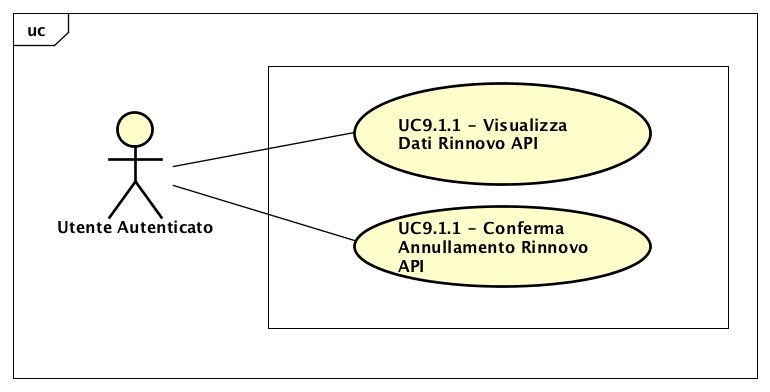
\includegraphics[scale=0.45]{UML/UC9_1.png}
	\caption{UC9.1: Annullamento Rinnovo API}
\end{figure}
\FloatBarrier
\renewcommand*{\arraystretch}{1.6}
\begin{longtable}{ l | p{11cm}}
	\hline
	\rowcolor{Gray}
	\multicolumn{2}{c}{UC9.1: Annullamento Rinnovo API} \\
	\hline
	\textbf{Attori} &Utente Autenticato, Amministratore APIMarket, Interfacce API Presente In APIMarket \\
	\textbf{Descrizione} & l'attore sceglie attraverso quale modalità interagire con le API acquistate \\
	\textbf{Pre-Condizioni} & l'attore ha scelto di gestire il rinnovo automatico di una API\\
	\textbf{Post-Condizioni}&l'attore ha effettuato le operazioni desiderate\\
	\textbf{Scenario Principale} & \begin{enumerate*}[label=(\arabic*.),itemjoin={\newline}]
		\item L'attore può visualizzare i dati riguardanti il rinnovo automatico di una API (UC9.1.1);
		\item L'attore può confermare l'annullamento del rinnovo automatico di una API (UC9.1.2)
	\end{enumerate*}\\
\end{longtable}


%\paragraph{Caso d'uso UC9.1.1: Visualizzazione Dati Rinnovo API}
\label{UC9.1.1}

\renewcommand*{\arraystretch}{1.6}
\begin{longtable}{ l | p{11cm}}
	\hline
	\rowcolor{Gray}
	\multicolumn{2}{c}{UC9.1.1: Visualizzazione Dati Rinnovo API} \\
	\hline
	\textbf{Attori} &Utente Autenticato, Amministratore APIMarket, Interfacce API Presente In APIMarket \\
	\textbf{Descrizione} & l'attore visualizza i dati del rinnovo automatico di una API acquistata \\
	\textbf{Pre-Condizioni} &  l'attore ha scelto di visualizzare i dati del rinnovo automatico di una API acquistata\\
	\textbf{Post-Condizioni}& l'attore ha visualizzato i dati del rinnovo automatico di una API acquistata\\
	\textbf{Scenario Principale} & \begin{enumerate*}[label=(\arabic*.),itemjoin={\newline}]
		\item L'attore può visualizzare i dati riguardanti il rinnovo automatico di una API
	\end{enumerate*}\\
\end{longtable}

%\newpage
\paragraph{Caso d'uso UC9.1.2: Conferma Annullamento Rinnovo API}
\label{UC9.1.2}

\renewcommand*{\arraystretch}{1.6}
\begin{longtable}{ l | p{11cm}}
	\hline
	\rowcolor{Gray}
	\multicolumn{2}{c}{UC9.1.2: Conferma Annullamento Rinnovo API} \\
	\hline
	\textbf{Attori} &Utente Autenticato, Amministratore APIMarket, Interfacce API Presente In APIMarket \\
	\textbf{Descrizione} & l'attore conferma l'annullamento del rinnovo automatico di una API acquistata \\
	\textbf{Pre-Condizioni} & l'attore ha scelto di confermare l'annullamento del rinnovo automatico di una API acquistata\\
	\textbf{Post-Condizioni}& l'attore ha confermato l'annullamento del rinnovo automatico di una API acquistata\\
	\textbf{Scenario Principale} & \begin{enumerate*}[label=(\arabic*.),itemjoin={\newline}]
		\item l'attore può confermare l'annullamento del rinnovo automatico di una API acquistata
	\end{enumerate*}\\
\end{longtable}

%\subsubsection{Caso d'uso UC9.2: Interazione Interfaccia API}
\label{UC9.2}

\renewcommand*{\arraystretch}{1.6}
\begin{longtable}{ l | p{11cm}}
	\hline
	\rowcolor{Gray}
	\multicolumn{2}{c}{UC9.2: Interazione Interfaccia API} \\
	\hline
	\textbf{Attori} &Utente Autenticato, Amministratore APIMarket, Interfacce API Presente In APIMarket \\
	\textbf{Descrizione} & l'attore interagisce con l'interfaccia API \\
	\textbf{Pre-Condizioni} & l'attore ha scelto di interagire con l'interfaccia API acquistata\\
	\textbf{Post-Condizioni}& l'attore ha finito di interagire con l'interfaccia API acquistata\\
	\textbf{Scenario Principale} & \begin{enumerate*}[label=(\arabic*.),itemjoin={\newline}]
			\item l'attore può interagire con l'interfaccia di una API acquistata
	\end{enumerate*}\\
\end{longtable}
%\subsubsection{Caso d'uso UC9.3: Rimozione API Dalle API Acquistate}
\label{UC9.3}

\renewcommand*{\arraystretch}{1.6}
\begin{longtable}{ l | p{11cm}}
	\hline
	\rowcolor{Gray}
	\multicolumn{2}{c}{UC9.3: Rimozione API Dalle API Acquistate} \\
	\hline
	\textbf{Attori} &Utente Autenticato, Amministratore APIMarket, Interfacce API Presente In APIMarket \\
	\textbf{Descrizione} & l'attore sceglie se rimuovere una API dalle API acquistate \\
	\textbf{Pre-Condizioni} & l'attore ha scelto di rimuovere una API dalle API acquistate\\
	\textbf{Post-Condizioni}& l'attore ha rimosso una API dalle API acquistate oppure ha annullato l'operazione\\
	\textbf{Scenario Principale} & \begin{enumerate*}[label=(\arabic*.),itemjoin={\newline}]
			\item l'attore può confermare la rimozione di una API dalle API acquistate
	\end{enumerate*}\\
\end{longtable}



%\subsubsection{Caso d'uso UC9.4: Visualizzazione Scadenza API}
\label{UC9.4}

\renewcommand*{\arraystretch}{1.6}
\begin{longtable}{ l | p{11cm}}
	\hline
	\rowcolor{Gray}
	\multicolumn{2}{c}{UC9.4: Visualizzazione Scadenza API} \\
	\hline
	\textbf{Attori} &Utente Autenticato, Amministratore APIMarket, Interfacce API Presente In APIMarket \\
	\textbf{Descrizione} & l'attore visualizza la data di scadenza della chiave di una API \\
	\textbf{Pre-Condizioni} &l'attore ha scelto di visualizzare la scadenza di una API\\
	\textbf{Post-Condizioni}& l'attore ha visualizzato la scadenza di una API\\
	\textbf{Scenario Principale} & \begin{enumerate*}[label=(\arabic*.),itemjoin={\newline}]
		\item L'attore può visualizzare la data di scadenza della chiave di una API
	\end{enumerate*}\\
\end{longtable}
%\newpage
\subsection{Caso d'uso UC10: Visualizzazione API registrate}
\label{UC10}
\begin{figure}[ht]
	\centering
	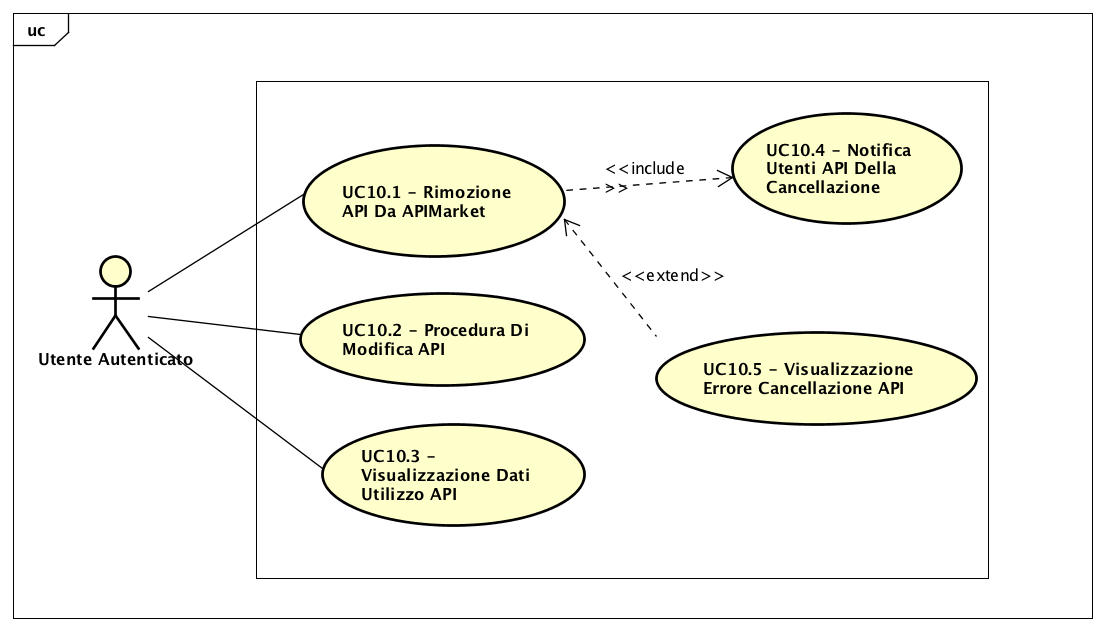
\includegraphics[scale=0.45]{UML/UC10.png}
	\caption{UC10: Visualizzazione API registrate}
\end{figure}

\begin{longtable}{ l | p{11cm}}
	\hline
	\rowcolor{Gray}
	\multicolumn{2}{c}{UC10 - Visualizzazione API registrate}\\
	\hline
	\textbf{Attori} & Utente autenticato, Amministratore API Market \\
	\textbf{Descrizione} & L'attore visualizza le API da lui registrate \\
	\textbf{Pre-Condizioni} & L'attore si trova nella schermata relativa alle API da lui registrate \\
	\textbf{Post-Condizioni} & L'attore ha visualizzato le API da lui registrate \\
	\textbf{Scenario Principale} & 
	\begin{enumerate*}[label=(\arabic*.),itemjoin={\newline}]
		\item L'attore può visualizzare il numero delle API da lui registrate (UC10.1)
		\item L'attore può visualizzare la lista delle API da lui registrate (UC10.2)
	\end{enumerate*}\\
	\textbf{Scenari Alternativi} & 
	\begin{enumerate*}[label=(\arabic*.),itemjoin={\newline}]
		\item L'attore può visualizzare i dati relativi ad ogni API (UC7)
	\end{enumerate*}\\
\end{longtable}

\subsubsection{Caso d'uso UC10.1: Visualizzazione numero API registrate}
\label{UC10_1}

\begin{minipage}{\linewidth}
	\begin{tabular}{ l | p{11cm}}
		\hline
		\rowcolor{Gray}
		\multicolumn{2}{c}{UC10.1 - Visualizzazione numero API registrate} \\
		\hline
		\textbf{Attori} & Utente autenticato, Amministratore API Market \\
		\textbf{Descrizione} & L'attore visualizza il numero di API da lui registrate \\
		\textbf{Pre-Condizioni} & L'attore si trova nella schermata relativa alle API da lui registrate \\
		\textbf{Post-Condizioni} & L'attore ha visualizzato il numero delle API da lui registrate \\
		\textbf{Scenario Principale} & 
		\begin{enumerate*}[label=(\arabic*.),itemjoin={\newline}]
			\item L'attore può visualizzare il numero di API da lui registrate
		\end{enumerate*}\\
	\end{tabular}
\end{minipage}

\newpage
\subsubsection{Caso d'uso UC10.2: Visualizzazione lista API registrate}
\label{UC10_2}
\begin{figure}[ht]
	\centering
	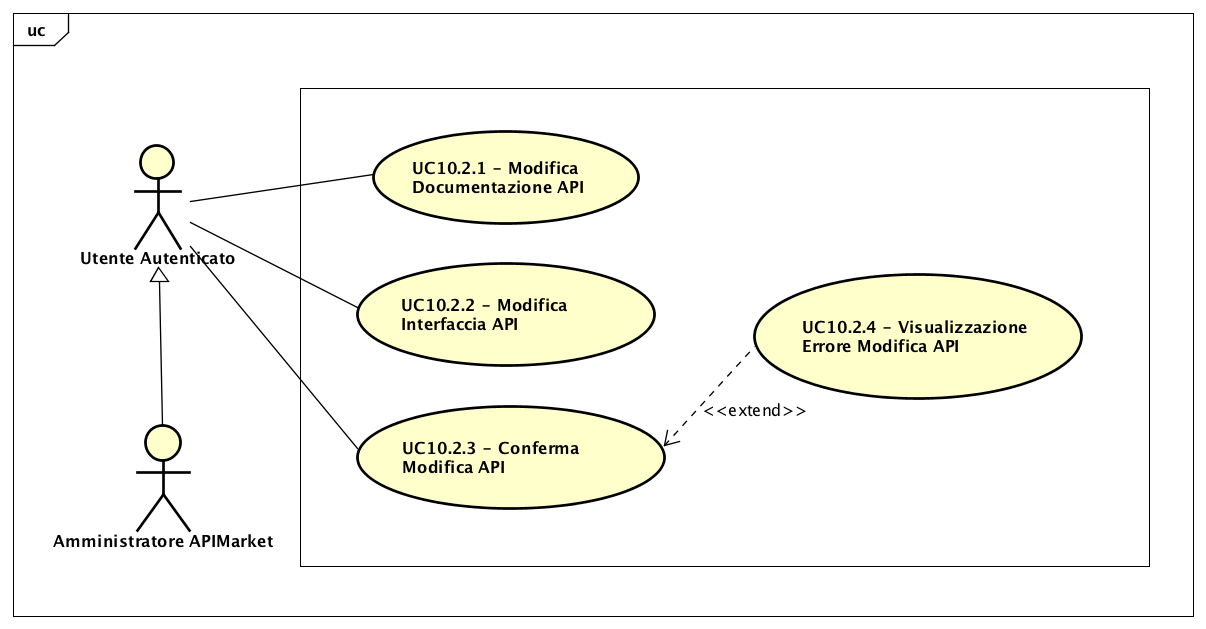
\includegraphics[scale=0.45]{UML/UC10_2.png}
	\caption{UC10.2: Visualizzazione lista API registrate}
\end{figure}

\begin{minipage}{\linewidth}
	\begin{tabular}{ l | p{11cm}}
		\hline
		\rowcolor{Gray}
		\multicolumn{2}{c}{UC10.2 - Visualizzazione lista API registrate} \\
		\hline
		\textbf{Attori} & Utente autenticato, Amministratore API Market \\
		\textbf{Descrizione} & L'attore visualizza la lista di ogni API da lui registrata \\
		\textbf{Pre-Condizioni} & L'attore si trova nella schermata relativa alle API da lui registrate \\
		\textbf{Post-Condizioni} & L'attore ha visualizzato la lista delle API da lui registrate \\
		\textbf{Scenario Principale} & 
		\begin{enumerate*}[label=(\arabic*.),itemjoin={\newline}]
			\item L'attore può visualizzare il nome di ogni API da lui registrata (UC10.2.1)
			\item L'attore può visualizzare il link alla pagina di visualizzazione API di ogni API da lui registrata (UC10.2.2)
			\item L'attore può visualizzare il numero di licenze attive di ogni API da lui registrata (UC10.2.3)
			\item L'attore può modificare ogni API da lui registrata (UC10.2.4)
			\item L'attore può eliminare ogni API da lui registrata (UC10.2.5)
		\end{enumerate*}\\
	\end{tabular}
\end{minipage}

\paragraph{Caso d'uso UC10.2.1: Visualizzazione nome API}
\label{UC10_2_1}

\begin{minipage}{\linewidth}
	\begin{tabular}{ l | p{11cm}}
		\hline
		\rowcolor{Gray}
		\multicolumn{2}{c}{UC10.2.1 - Visualizzazione nome API} \\
		\hline
		\textbf{Attori} & Utente autenticato, Amministratore API Market \\
		\textbf{Descrizione} & L'attore visualizza nella lista il nome di ogni API da lui registrata \\
		\textbf{Pre-Condizioni} & L'attore si trova nella schermata relativa alle API da lui registrate \\
		\textbf{Post-Condizioni} & L'attore ha visualizzato nella lista il nome di ogni API da lui registrata \\
		\textbf{Scenario Principale} & 
		\begin{enumerate*}[label=(\arabic*.),itemjoin={\newline}]
			\item L'attore può visualizzare nella lista il nome di ogni API da lui registrata
		\end{enumerate*}\\
	\end{tabular}
\end{minipage}

\paragraph{Caso d'uso UC10.2.2: Visualizzazione link API}
\label{UC10_2_2}

\begin{minipage}{\linewidth}
	\begin{tabular}{ l | p{11cm}}
		\hline
		\rowcolor{Gray}
		\multicolumn{2}{c}{UC10.2.2 - Visualizzazione link API} \\
		\hline
		\textbf{Attori} & Utente autenticato, Amministratore API Market \\
		\textbf{Descrizione} & L'attore visualizza nella lista il link alla visualizzazione di ogni API da lui registrata \\
		\textbf{Pre-Condizioni} & L'attore si trova nella schermata relativa alle API da lui registrate \\
		\textbf{Post-Condizioni} & L'attore ha visualizzato nella lista il link alla visualizzazione di ogni API da lui registrata \\
		\textbf{Scenario Principale} & 
		\begin{enumerate*}[label=(\arabic*.),itemjoin={\newline}]
			\item L'attore può visualizzare nella lista il link alla visualizzazione di ogni API da lui registrata
		\end{enumerate*}\\
	\end{tabular}
\end{minipage}

\paragraph{Caso d'uso UC10.2.3: Visualizzazione numero licenze attive}
\label{UC10_2_3}

\begin{minipage}{\linewidth}
	\begin{tabular}{ l | p{11cm}}
		\hline
		\rowcolor{Gray}
		\multicolumn{2}{c}{UC10.2.3 - Visualizzazione numero licenze attive} \\
		\hline
		\textbf{Attori} & Utente autenticato, Amministratore API Market \\
		\textbf{Descrizione} & L'attore visualizza nella lista il numero di licenze attive per ogni API da lui registrata \\
		\textbf{Pre-Condizioni} & L'attore si trova nella schermata relativa alle API da lui registrate \\
		\textbf{Post-Condizioni} & L'attore ha visualizzato nella lista il numero di licenze attive per ogni API da lui registrata \\
		\textbf{Scenario Principale} & 
		\begin{enumerate*}[label=(\arabic*.),itemjoin={\newline}]
			\item L'attore può visualizzare nella lista il numero di licenze attive per ogni API da lui registrata
		\end{enumerate*}\\
	\end{tabular}
\end{minipage}

\paragraph{Caso d'uso UC10.2.4: Notifica eliminazione API}
\label{UC10_2_1}

\begin{minipage}{\linewidth}
	\begin{tabular}{ l | p{11cm}}
		\hline
		\rowcolor{Gray}
		\multicolumn{2}{c}{UC10.2.1 - Notifica eliminazione API} \\
		\hline
		\textbf{Attori} & Utente autenticato, Amministratore API Market \\
		\textbf{Descrizione} & Per ogni API da lui registrata nella lista, l'attore visualizza se questa sia in fase di eliminazione \\
		\textbf{Pre-Condizioni} & L'attore si trova nella schermata relativa alle API da lui registrate \\
		\textbf{Post-Condizioni} & Per ogni API da lui registrata nella lista, l'attore ha visualizzato se questa sia in fase di eliminazione \\
		\textbf{Scenario Principale} & 
		\begin{enumerate*}[label=(\arabic*.),itemjoin={\newline}]
			\item Per ogni API da lui registrata nella lista, l'attore può visualizzare se questa sia in fase di eliminazione
		\end{enumerate*}\\
	\end{tabular}
\end{minipage}

\newpage
\paragraph{Caso d'uso UC10.2.5: Modifica API registrata}
\label{UC10_2_5}
\begin{figure}[ht]
	\centering
	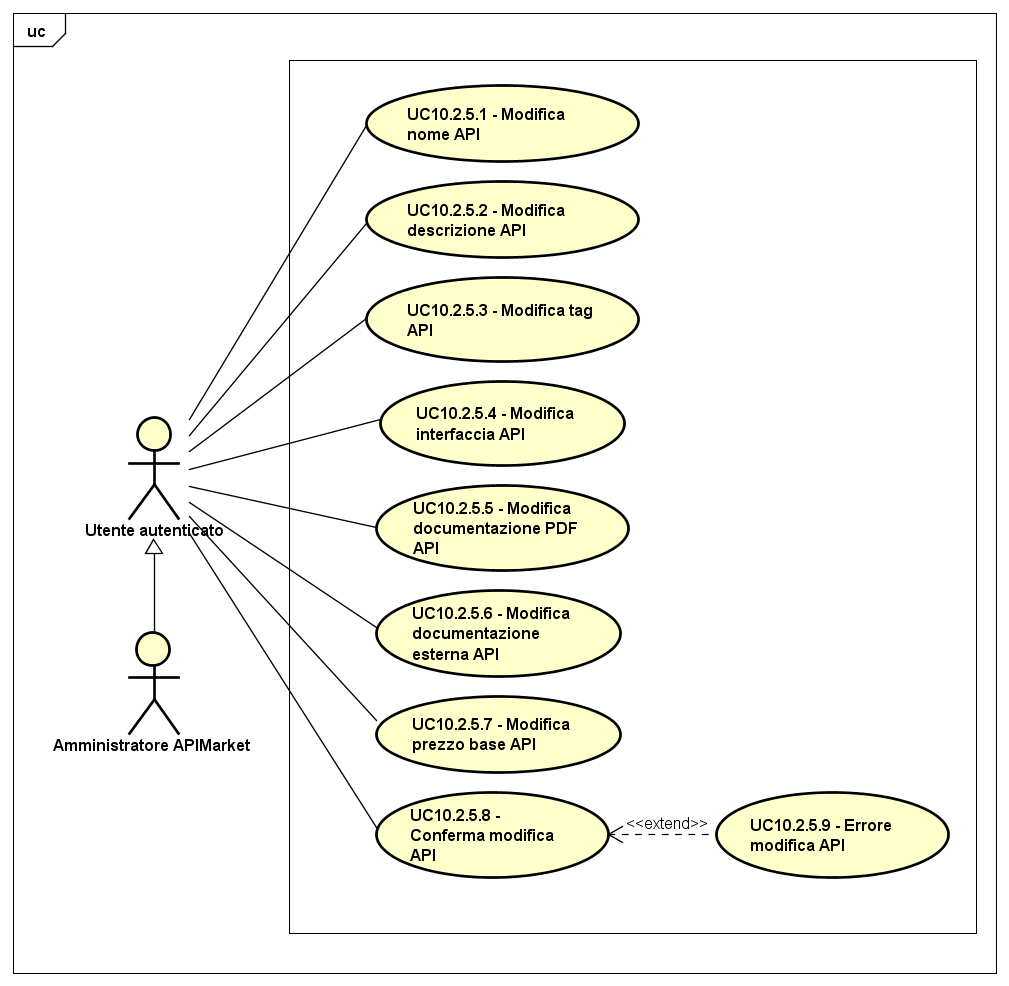
\includegraphics[scale=0.45]{UML/UC10_2_5.png}
	\caption{UC10.2.5: Modifica API registrata}
\end{figure}

\begin{minipage}{\linewidth}
	\begin{tabular}{ l | p{11cm}}
		\hline
		\rowcolor{Gray}
		\multicolumn{2}{c}{UC10.2.5 - Modifica API registrata} \\
		\hline
		\textbf{Attori} & Utente autenticato, Amministratore API Market \\
		\textbf{Descrizione} & L'attore modifica una API da lui registrata \\
		\textbf{Pre-Condizioni} & L'attore si trova nella schermata relativa alle API da lui registrate \\
		\textbf{Post-Condizioni} & L'attore ha modificato un API registrata \\
		\textbf{Scenario Principale} & 
		\begin{enumerate*}[label=(\arabic*.),itemjoin={\newline}]
			\item L'attore può modificare il nome dell'API (UC10.2.5.1)
			\item L'attore può modificare la descrizione dell'API (UC10.2.5.2)
			\item L'attore può modificare i tag dell'API (UC10.2.5.3)
			\item L'attore può modificare l'interfaccia dell'API (UC10.2.5.4)
			\item L'attore può modificare il file per la documentazione PDF (UC10.2.5.5)
			\item L'attore può modificare il link per la documentazione esterna (UC10.2.5.6)
			\item L'attore può modificare il prezzo base dell'API (UC10.2.5.7)
			\item L'attore può confermare la modifica dell'API (UC10.2.5.8)
		\end{enumerate*}\\
		\textbf{Scenari Alternativi} & 
		\begin{enumerate*}[label=(\arabic*.),itemjoin={\newline}]
			\item L'attore può visualizzare un messaggio d'errore informativo riguardo la conferma delle modifiche dell'API, e le modifiche non avvengono (UC10.2.5.9)
			\item L'attore può visualizzare un messaggio di errore riguardo al caricamento del file di documentazione PDF dell'API, ed il caricamento del file non avviene (UC10.2.5.10)
		\end{enumerate*}\\
	\end{tabular}
\end{minipage}

\subparagraph{Caso d'uso UC10.2.5.1: Modifica nome API}
\label{UC10_2_5_1}

\begin{minipage}{\linewidth}
	\begin{tabular}{ l | p{11cm}}
		\hline
		\rowcolor{Gray}
		\multicolumn{2}{c}{UC10.2.5.1 - Modifica nome API} \\
		\hline
		\textbf{Attori} & Utente autenticato, Amministratore API Market \\
		\textbf{Descrizione} & L'attore modifica il nome dell'API \\
		\textbf{Pre-Condizioni} & L'attore si trova nella schermata relativa alla modifica di una API registrata, precedentemente selezionata \\
		\textbf{Post-Condizioni} & L'attore ha modificato il nome dell'API selezionata \\
		\textbf{Scenario Principale} & 
		\begin{enumerate*}[label=(\arabic*.),itemjoin={\newline}]
			\item L'attore può modificare il nome dell'API
		\end{enumerate*}\\
	\end{tabular}
\end{minipage}

\subparagraph{Caso d'uso UC10.2.5.2: Modifica descrizione API}
\label{UC10_2_5_2}

\begin{minipage}{\linewidth}
	\begin{tabular}{ l | p{11cm}}
		\hline
		\rowcolor{Gray}
		\multicolumn{2}{c}{UC10.2.5.2 - Modifica descrizione API} \\
		\hline
		\textbf{Attori} & Utente autenticato, Amministratore API Market \\
		\textbf{Descrizione} & L'attore modifica la descrizione dell'API\\
		\textbf{Pre-Condizioni} & L'attore si trova nella schermata relativa alla modifica di una API registrata, precedentemente selezionata \\
		\textbf{Post-Condizioni} & L'attore ha modificato la descrizione dell'API selezionata \\
		\textbf{Scenario Principale} & 
		\begin{enumerate*}[label=(\arabic*.),itemjoin={\newline}]
			\item L'attore può modificare la descrizione dell'API
		\end{enumerate*}\\
	\end{tabular}
\end{minipage}

\subparagraph{Caso d'uso UC10.2.5.3: Modifica tag API}
\label{UC10_2_5_3}

\begin{minipage}{\linewidth}
	\begin{tabular}{ l | p{11cm}}
		\hline
		\rowcolor{Gray}
		\multicolumn{2}{c}{UC10.2.5.3 - Modifica tag API} \\
		\hline
		\textbf{Attori} & Utente autenticato, Amministratore API Market \\
		\textbf{Descrizione} & L'attore modifica i tag dell'API \\
		\textbf{Pre-Condizioni} & L'attore si trova nella schermata relativa alla modifica di una API registrata, precedentemente selezionata \\
		\textbf{Post-Condizioni} & L'attore ha modificato i tag dell'API selezionata \\
		\textbf{Scenario Principale} & 
		\begin{enumerate*}[label=(\arabic*.),itemjoin={\newline}]
			\item L'attore può modificare i tag dell'API
		\end{enumerate*}\\
	\end{tabular}
\end{minipage}

\subparagraph{Caso d'uso UC10.2.5.4: Modifica interfaccia API}
\label{UC10_2_5_4}

\begin{minipage}{\linewidth}
	\begin{tabular}{ l | p{11cm}}
		\hline
		\rowcolor{Gray}
		\multicolumn{2}{c}{UC10.2.5.4 - Modifica interfaccia API} \\
		\hline
		\textbf{Attori} & Utente autenticato, Amministratore API Market \\
		\textbf{Descrizione} & L'attore modifica l'interfaccia dell'API \\
		\textbf{Pre-Condizioni} & L'attore si trova nella schermata relativa alla modifica di una API registrata, precedentemente selezionata \\
		\textbf{Post-Condizioni} & L'attore ha modificato l'interfaccia pubblica dell'API selezionata \\
		\textbf{Scenario Principale} & 
		\begin{enumerate*}[label=(\arabic*.),itemjoin={\newline}]
			\item L'attore può modificare l'interfaccia dell'API
		\end{enumerate*}\\
	\end{tabular}
\end{minipage}

\subparagraph{Caso d'uso UC10.2.5.5: Modifica documentazione PDF API}
\label{UC10_2_5_5}

\begin{minipage}{\linewidth}
	\begin{tabular}{ l | p{11cm}}
		\hline
		\rowcolor{Gray}
		\multicolumn{2}{c}{UC10.2.5.5 - Modifica documentazione PDF API} \\
		\hline
		\textbf{Attori} & Utente autenticato, Amministratore API Market \\
		\textbf{Descrizione} & L'attore carica su API Market un file PDF contenente la nuova documentazione PDF dell'API \\
		\textbf{Pre-Condizioni} & L'attore si trova nella schermata relativa alla modifica di una API registrata, precedentemente selezionata \\
		\textbf{Post-Condizioni} & L'attore ha caricato su API Market un nuovo file PDF contenente la documentazione PDF dell'API \\
		\textbf{Scenario Principale} & 
		\begin{enumerate*}[label=(\arabic*.),itemjoin={\newline}]
			\item L'attore può caricare su API Market un nuovo file PDF contenente la documentazione PDF dell'API
		\end{enumerate*}\\
		\textbf{Scenari Alternativi} & 
		\begin{enumerate*}[label=(\arabic*.),itemjoin={\newline}]
			\item L'attore può visualizzare un messaggio di errore ed il caricamento del file non avviene (UC10.2.5.10)
		\end{enumerate*}\\
	\end{tabular}
\end{minipage}

\subparagraph{Caso d'uso UC10.2.5.10: Errore modifica PDF API}
\label{UC10_2_5_10}

\begin{minipage}{\linewidth}
	\begin{tabular}{ l | p{11cm}}
		\hline
		\rowcolor{Gray}
		\multicolumn{2}{c}{UC10.2.5.10 - Errore modifica PDF API} \\
		\hline
		\textbf{Attori} & Utente autenticato, Amministratore API Market \\
		\textbf{Descrizione} & L'attore visualizza un messaggio di errore e la modifica della documentazione PDF dell'API non avviene \\
		\textbf{Pre-Condizioni} & L'attore ha cercato di caricare su API Market un file contenente la documentazione dell'API ma si è verificato un errore \\
		\textbf{Post-Condizioni} & L'attore ha visualizzato un messaggio di errore \\
		\textbf{Scenario Principale} & 
		\begin{enumerate*}[label=(\arabic*.),itemjoin={\newline}]
			\item L'attore può visualizzare un messaggio di errore
		\end{enumerate*}\\
	\end{tabular}
\end{minipage}

\subparagraph{Caso d'uso UC10.2.5.6: Modifica documentazione esterna API}
\label{UC10_2_5_6}

\begin{minipage}{\linewidth}
	\begin{tabular}{ l | p{11cm}}
		\hline
		\rowcolor{Gray}
		\multicolumn{2}{c}{UC10.2.5.6 - Modifica documentazione esterna API} \\
		\hline
		\textbf{Attori} & Utente autenticato, Amministratore API Market \\
		\textbf{Descrizione} & L'attore modifica il link alla documentazione esterna dell'API \\
		\textbf{Pre-Condizioni} & L'attore si trova nella schermata relativa alla modifica di una API registrata, precedentemente selezionata \\
		\textbf{Post-Condizioni} & L'attore ha modificato il link alla documentazione esterna dell'API selezionata \\
		\textbf{Scenario Principale} & 
		\begin{enumerate*}[label=(\arabic*.),itemjoin={\newline}]
			\item L'attore può modificare il link alla documentazione esterna dell'API
		\end{enumerate*}\\
	\end{tabular}
\end{minipage}

\subparagraph{Caso d'uso UC10.2.5.7: Modifica prezzo base API}
\label{UC10_2_5_7}

\begin{minipage}{\linewidth}
	\begin{tabular}{ l | p{11cm}}
		\hline
		\rowcolor{Gray}
		\multicolumn{2}{c}{UC10.2.5.7 - Modifica prezzo base API} \\
		\hline
		\textbf{Attori} & Utente autenticato, Amministratore API Market \\
		\textbf{Descrizione} & L'attore modifica il prezzo base dell'API \\
		\textbf{Pre-Condizioni} & L'attore si trova nella schermata relativa alla modifica di una API registrata, precedentemente selezionata \\
		\textbf{Post-Condizioni} & L'attore ha modificato prezzo base dell'API selezionata \\
		\textbf{Scenario Principale} & 
		\begin{enumerate*}[label=(\arabic*.),itemjoin={\newline}]
			\item L'attore può modificare prezzo base dell'API
		\end{enumerate*}\\
	\end{tabular}
\end{minipage}

\subparagraph{Caso d'uso UC10.2.5.8: Conferma modifica API}
\label{UC10_2_5_8}

\begin{minipage}{\linewidth}
	\begin{tabular}{ l | p{11cm}}
		\hline
		\rowcolor{Gray}
		\multicolumn{2}{c}{UC10.2.5.8 - Conferma modifica API} \\
		\hline
		\textbf{Attori} & Utente autenticato, Amministratore API Market \\
		\textbf{Descrizione} & L'attore conferma le modifiche all'API, visualizzando un messaggio di successo \\
		\textbf{Pre-Condizioni} & L'attore si trova nella schermata relativa alla modifica di una API registrata, precedentemente selezionata \\
		\textbf{Post-Condizioni} & L'attore ha confermato le modifiche all'API, visualizzando un messaggio di successo \\
		\textbf{Scenario Principale} & 
		\begin{enumerate*}[label=(\arabic*.),itemjoin={\newline}]
			\item L'attore può confermare le modifiche effettuate all'API, visualizzando un messaggio di successo e venendo reindirizzato alla schermata di visualizzazione API registrate (UC10)
		\end{enumerate*}\\
	\end{tabular}
\end{minipage}

\subparagraph{Caso d'uso UC10.2.5.9: Errore modifica API}
\label{UC10_2_5_9}

\begin{minipage}{\linewidth}
	\begin{tabular}{ l | p{11cm}}
		\hline
		\rowcolor{Gray}
		\multicolumn{2}{c}{UC10.2.5.9 - Errore modifica API} \\
		\hline
		\textbf{Attori} & Utente autenticato, Amministratore API Market \\
		\textbf{Descrizione} & L'attore visualizza un messaggio di errore informativo e la modifica dell'API non avviene \\
		\textbf{Pre-Condizioni} & L'attore ha confermato la modifica di una API ma si è verificato un errore \\
		\textbf{Post-Condizioni} & L'attore ha visualizzato un messaggio di errore informativo \\
		\textbf{Scenario Principale} & 
		\begin{enumerate*}[label=(\arabic*.),itemjoin={\newline}]
			\item L'attore può visualizzare un messaggio di errore informativo e la modifica non avviene
		\end{enumerate*}\\
	\end{tabular}
\end{minipage}

\paragraph{Caso d'uso UC10.2.6: Eliminazione API registrata}
\label{UC10_2_6}

\begin{minipage}{\linewidth}
	\begin{tabular}{ l | p{11cm}}
		\hline
		\rowcolor{Gray}
		\multicolumn{2}{c}{UC10.2.6 - Eliminazione API registrata} \\
		\hline
		\textbf{Attori} & Utente autenticato, Amministratore API Market \\
		\textbf{Descrizione} & L'attore richiede l'eliminazione di una API da lui registrata, che verrà eliminata secondo le politiche di API Market \\
		\textbf{Pre-Condizioni} & L'attore si trova nella schermata relativa alle API da lui registrate \\
		\textbf{Post-Condizioni} & L'attore ha richiesto l'eliminazione di una API da lui registrata \\
		\textbf{Scenario Principale} & 
		\begin{enumerate*}[label=(\arabic*.),itemjoin={\newline}]
			\item L'attore può richiedere l'eliminazione di una API da lui registrata, che verrà eliminata secondo le politiche di API Market
		\end{enumerate*}\\
	\end{tabular}
\end{minipage}

\paragraph{Caso d'uso UC10.2.7: Revoca eliminazione API registrata}
\label{UC10_2_7}

\begin{minipage}{\linewidth}
	\begin{tabular}{ l | p{11cm}}
		\hline
		\rowcolor{Gray}
		\multicolumn{2}{c}{UC10.2.7 - Revoca eliminazione API registrata} \\
		\hline
		\textbf{Attori} & Utente autenticato, Amministratore API Market \\
		\textbf{Descrizione} & L'attore revoca la richiesta di eliminazione di una API da lui registrata \\
		\textbf{Pre-Condizioni} & L'attore si trova nella schermata relativa alle API da lui registrate \\
		\textbf{Post-Condizioni} & L'attore ha revocato la richiesta di eliminazione di una API da lui registrata \\
		\textbf{Scenario Principale} & 
		\begin{enumerate*}[label=(\arabic*.),itemjoin={\newline}]
			\item L'attore può revocare la richiesta di eliminazione di una API da lui registrata
		\end{enumerate*}\\
	\end{tabular}
\end{minipage}
%\subsubsection{Caso d'uso UC10.1: Rimozione API Da APIMarket}
\label{UC10.1}

\renewcommand*{\arraystretch}{1.6}
\begin{longtable}{ l | p{11cm}}
	\hline
	\rowcolor{Gray}
	\multicolumn{2}{c}{UC10.1: Rimozione API Da APIMarket} \\
	\hline
	\textbf{Attori} &Utente Autenticato, Amministratore APIMarket \\
	\textbf{Descrizione} & l'attore rimuove dall'APIMarket una propria API\\
	\textbf{Pre-Condizioni} & l'attore ha scelto di rimuovere dall'APIMarket una propria API\\
	\textbf{Post-Condizioni}&l'attore ha rimosso dall'APIMarket una propria API\\
	\textbf{Scenario Principale} & \begin{enumerate*}[label=(\arabic*.),itemjoin={\newline}]
			\item L'attore può rimuovere dall'APIMarket una propria API
	\end{enumerate*}\\
\end{longtable}




%\subsubsection{Caso d'uso UC10.2: Modifica API}
\label{UC10.2}

\begin{figure}[ht]
	\centering
	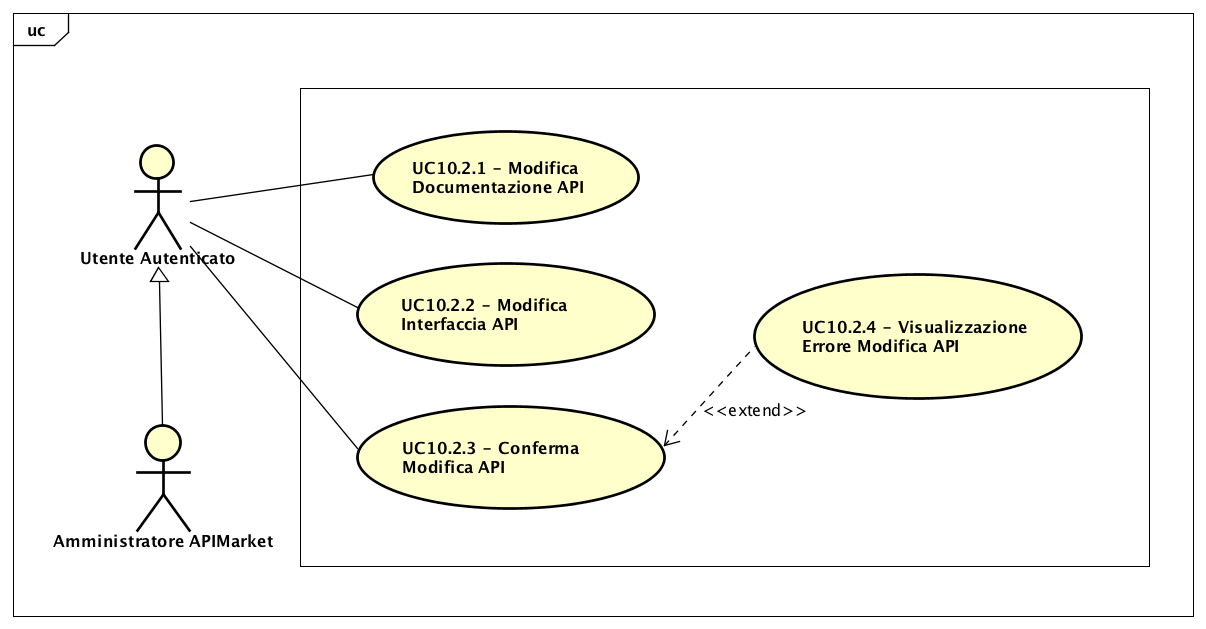
\includegraphics[scale=0.45]{UML/UC10_2.png}
	\caption{UC10.2: Modifica API}
\end{figure}

\renewcommand*{\arraystretch}{1.6}
\begin{longtable}{ l | p{11cm}}
	\hline
	\rowcolor{Gray}
	\multicolumn{2}{c}{UC10.2: Modifica API} \\
	\hline
	\textbf{Attori} &Utente Autenticato, Amministratore APIMarket \\
	\textbf{Descrizione} & l'attore modifica una propria API\\
	\textbf{Pre-Condizioni} & l'attore ha scelto di modificare una propria API\\
	\textbf{Post-Condizioni}&l'attore ha modificato una propria API oppure l'operazione è fallita\\
	\textbf{Scenario Principale} & \begin{enumerate*}[label=(\arabic*.),itemjoin={\newline}]
		\item l'attore può modificare la documentazione della propria API (UC10.2.1)
		\item l'attore può modificare l'interfaccia della propria API (UC10.2.2)
		\item l'attore può confermare le modifiche alla propria API (UC10.2.3)
	\end{enumerate*}\\
	\textbf{Scenari Alternativi} & \begin{enumerate*}[label=(\arabic*.),itemjoin={\newline}]
		\item l'attore può visualizzare l'errore di modifica API (UC10.2.4)
	\end{enumerate*}\\
\end{longtable}

%\paragraph{Caso d'uso UC10.2.1: Modifica Documentazione API}
\label{UC10.2.1}

\renewcommand*{\arraystretch}{1.6}
\begin{longtable}{ l | p{11cm}}
	\hline
	\rowcolor{Gray}
	\multicolumn{2}{c}{UC10.2.1: Modifica Documentazione API} \\
	\hline
	\textbf{Attori} &Utente Autenticato, Amministratore APIMarket \\
	\textbf{Descrizione} &  l'attore modifica la documentazione della propria API\\
	\textbf{Pre-Condizioni} & l'attore ha scelto di modificare la documentazione della propria API\\
	\textbf{Post-Condizioni}& l'attore ha modificato la documentazione della propria API\\
	\textbf{Scenario Principale} & \begin{enumerate*}[label=(\arabic*.),itemjoin={\newline}]
		\item L'attore può rimuovere dall'APIMarket una propria API
	\end{enumerate*}\\
\end{longtable}




%\paragraph{Caso d'uso UC10.2.2: Modifica Interfaccia API}
\label{UC10.2.2}

\renewcommand*{\arraystretch}{1.6}
\begin{longtable}{ l | p{11cm}}
	\hline
	\rowcolor{Gray}
	\multicolumn{2}{c}{UC10.2.2: Modifica Interfaccia API} \\
	\hline
	\textbf{Attori} &Utente Autenticato, Amministratore APIMarket \\
	\textbf{Descrizione} &  l'attore modifica l'interfaccia della propria API\\
	\textbf{Pre-Condizioni} & l'attore ha scelto di modificare l'interfaccia della propria API\\
	\textbf{Post-Condizioni}& l'attore ha modificato l'interfaccia della propria API\\
	\textbf{Scenario Principale} & \begin{enumerate*}[label=(\arabic*.),itemjoin={\newline}]
		\item l'attore può modificare l'interfaccia della propria API
	\end{enumerate*}\\
\end{longtable}



%\paragraph{Caso d'uso UC10.2.3: Conferma Modifica API}
\label{UC10.2.3}

\renewcommand*{\arraystretch}{1.6}
\begin{longtable}{ l | p{11cm}}
	\hline
	\rowcolor{Gray}
	\multicolumn{2}{c}{UC10.2.3: Conferma Modifica API} \\
	\hline
	\textbf{Attori} &Utente Autenticato, Amministratore APIMarket \\
	\textbf{Descrizione} &  l'attore conferma le modifiche alla propria API\\
	\textbf{Pre-Condizioni} & l'attore ha scelto di confermare le modifiche alla propria API\\
	\textbf{Post-Condizioni}& l'attore ha confermato le modifiche alla propria API\\
	\textbf{Scenario Principale} & \begin{enumerate*}[label=(\arabic*.),itemjoin={\newline}]
		\item l'attore può confermare le modifiche alla propria API
	\end{enumerate*}\\
\end{longtable}



%\paragraph{Caso d'uso UC10.2.4: Visualizzazione Errore Modifica API}
\label{UC10.2.4}

\renewcommand*{\arraystretch}{1.6}
\begin{longtable}{ l | p{11cm}}
	\hline
	\rowcolor{Gray}
	\multicolumn{2}{c}{UC10.2.4: Visualizzazione Errore Modifica API} \\
	\hline
	\textbf{Attori} &Utente Autenticato, Amministratore APIMarket \\
	\textbf{Descrizione} &  l'attore visualizza l'errore nella modifica della propria API\\
	\textbf{Pre-Condizioni} & l'attore ha scelto di visualizzare l'errore nella modifica della propria API\\
	\textbf{Post-Condizioni}& l'attore ha visualizzato l'errore nella modifica della propria API ed è stato reindirizzato ad UC10.2\\
	\textbf{Scenario Principale} & \begin{enumerate*}[label=(\arabic*.),itemjoin={\newline}]
		\item l'attore può visualizzare l'errore nella modifica della propria API
	\end{enumerate*}\\
\end{longtable}



%\subsubsection{Caso d'uso UC10.3: Visualizzazione Dati Utilizzo API}
\label{UC10.3}

\renewcommand*{\arraystretch}{1.6}
\begin{longtable}{ l | p{11cm}}
	\hline
	\rowcolor{Gray}
	\multicolumn{2}{c}{UC10.3: Visualizzazione Dati Utilizzo API} \\
	\hline
	\textbf{Attori} &Utente Autenticato, Amministratore APIMarket \\
	\textbf{Descrizione} & l'attore visualizza i dati di utilizzo di una propria API\\
	\textbf{Pre-Condizioni} & l'attore ha scelto di visualizzare i dati di utilizzo di una propria API\\
	\textbf{Post-Condizioni}& l'attore ha visualizzato i dati di utilizzo di una propria API\\
	\textbf{Scenario Principale} & \begin{enumerate*}[label=(\arabic*.),itemjoin={\newline}]
		\item l'attore può visualizzare i dati di utilizzo di una propria API
	\end{enumerate*}\\
\end{longtable}

%\subsubsection{Caso d'uso UC10.4: Notifica Della Rimozione API}
\label{UC10.4}

\renewcommand*{\arraystretch}{1.6}
\begin{longtable}{ l | p{11cm}}
	\hline
	\rowcolor{Gray}
	\multicolumn{2}{c}{UC10.4: Notifica Della Rimozione API} \\
	\hline
	\textbf{Attori} &Utente Autenticato, Amministratore APIMarket \\
	\textbf{Descrizione} & l'applicazione web notifica gli utenti dell'API rimossa riguardo all'avvenuta rimozione\\
	\textbf{Pre-Condizioni} & l'attore ha rimosso dall'APIMarket una propria API\\
	\textbf{Post-Condizioni}& l'applicazione web ha notificato gli utenti dell'API rimossa riguardo all'avvenuta rimozione\\
	\textbf{Scenario Principale} & \begin{enumerate*}[label=(\arabic*.),itemjoin={\newline}]
		\item L'applicazione web può notificare gli utenti dell'API rimossa riguardo all'avvenuta rimozione
	\end{enumerate*}\\
\end{longtable}




%\subsubsection{Caso d'uso UC10.5: Visualizza Errore Cancellazione API}
\label{UC10.5}

\renewcommand*{\arraystretch}{1.6}
\begin{longtable}{ l | p{11cm}}
	\hline
	\rowcolor{Gray}
	\multicolumn{2}{c}{UC10.5: Visualizza Errore Cancellazione API} \\
	\hline
	\textbf{Attori} &Utente Autenticato, Amministratore APIMarket \\
	\textbf{Descrizione} & l'attore visualizza l'errore nella rimozione di una propria API\\
	\textbf{Pre-Condizioni} & l'attore ha tentato di rimuovere una propria API dall'APIMarket e l'operazione è fallita\\
	\textbf{Post-Condizioni}& l'attore ha visualizzato l'errore nella rimozione dell'API ed è stato reindirizzato ad UC10\\
	\textbf{Scenario Principale} & \begin{enumerate*}[label=(\arabic*.),itemjoin={\newline}]
		\item L'attore può visualizzare l'errore nella rimozione dell'API
	\end{enumerate*}\\
\end{longtable}



%\newpage
\subsection{Caso d'uso UC11 - Registrazione nuova API}
\label{UC11}
\begin{figure}[ht]
	\centering
	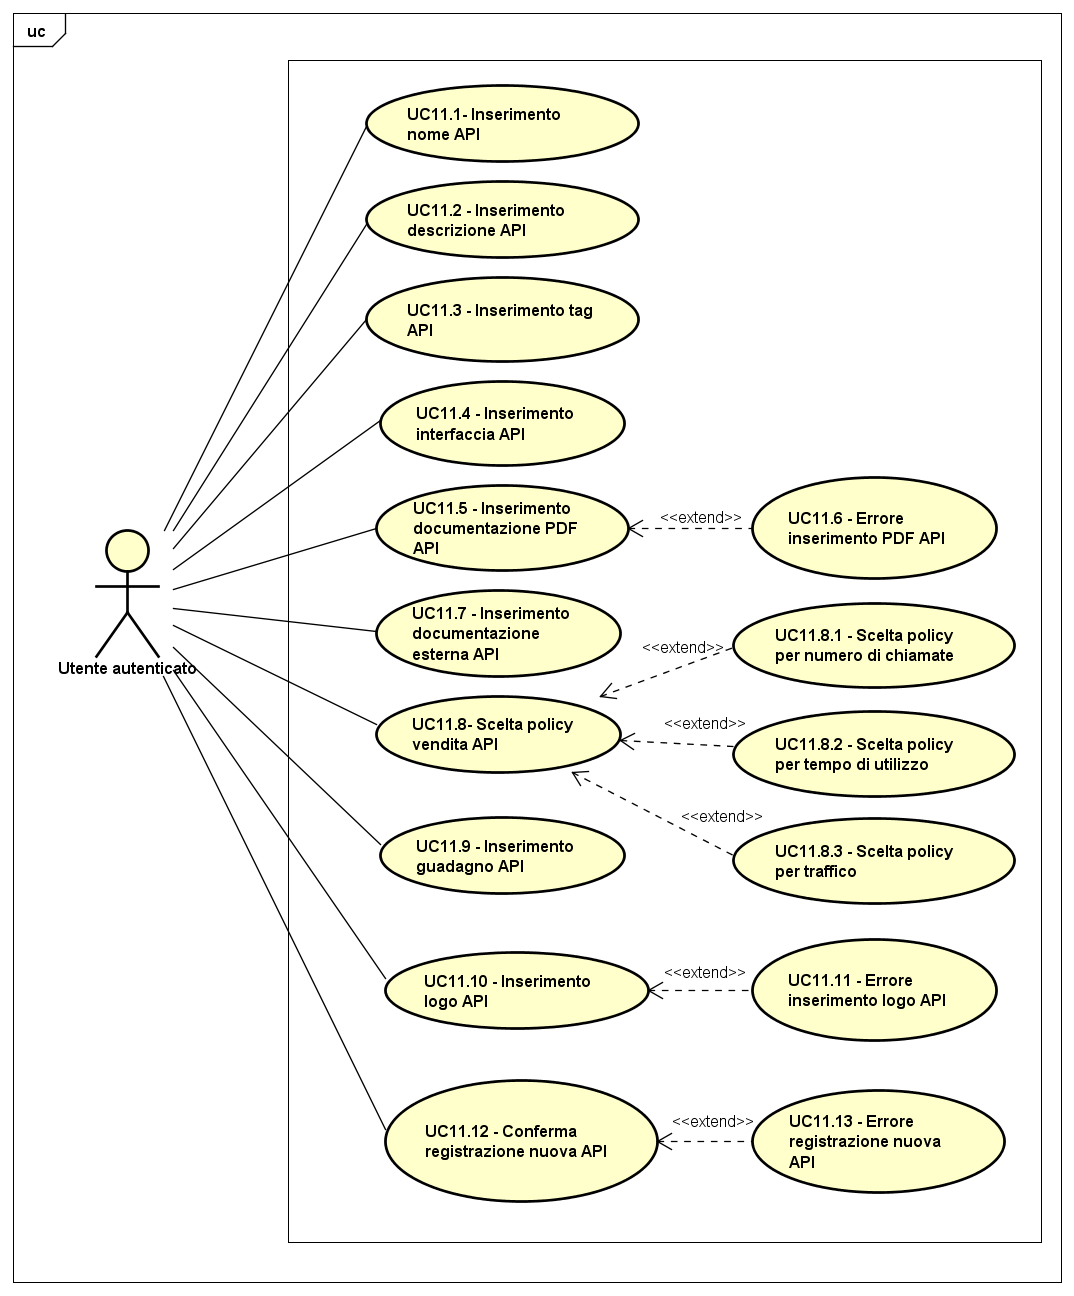
\includegraphics[scale=0.45]{UML/UC11.png}
	\caption{UC11: Registrazione nuova API}
\end{figure}

\begin{longtable}{ l | p{11cm}}
	\hline
	\rowcolor{Gray}
	\multicolumn{2}{c}{UC11 - Registrazione nuova API}\\
	\hline
	\textbf{Attori} & Utente autenticato, Amministratore API Market \\
	\textbf{Descrizione} & L'attore registra una nuova API su API Market \\
	\textbf{Pre-Condizioni} & L'attore si trova nella schermata relativa alla registrazione di una nuova API \\
	\textbf{Post-Condizioni} & L'attore ha registrato una nuova API su API Market \\
	\textbf{Scenario Principale} & 
	\begin{enumerate*}[label=(\arabic*.),itemjoin={\newline}]
		\item L'attore può inserire il nome della nuova API (UC11.1)
		\item L'attore può inserire la descrizione della nuova API (UC11.2)
		\item L'attore può inserire i tag della nuova API (UC11.3)
		\item L'attore può inserire l'interfaccia della nuova API (UC11.4)
		\item L'attore può inserire il file per la documentazione PDF della nuova API (UC11.5)
		\item L'attore può inserire il link per la documentazione esterna della nuova API (UC11.7)
		\item L'attore può inserire il prezzo base della nuova API (UC11.8)
		\item L'attore può confermare la registrazione della nuova API (UC11.9)
	\end{enumerate*}\\
	\textbf{Scenario Principale} & 
	\begin{enumerate*}[label=(\arabic*.),itemjoin={\newline}]
			\item L'attore può visualizzare un messaggio di errore riguardo al caricamento del file di documentazione PDF dell'API, ed il caricamento del file non avviene (UC11.6)
			\item L'attore può visualizzare un messaggio d'errore informativo riguardo la conferma della registrazione dell'API, e la registrazione non avviene (UC11.10)
	\end{enumerate*}\\
\end{longtable}

\subsubsection{Caso d'uso UC11.1: Inserimento nome API}
\label{UC11_1}

\begin{minipage}{\linewidth}
	\begin{tabular}{ l | p{11cm}}
		\hline
		\rowcolor{Gray}
		\multicolumn{2}{c}{UC11.1 - Inserimento nome API} \\
		\hline
		\textbf{Attori} & Utente autenticato, Amministratore API Market \\
		\textbf{Descrizione} & L'attore inserisce il nome della nuova API \\
		\textbf{Pre-Condizioni} & L'attore si trova nella schermata relativa alla registrazione di una nuova API \\
		\textbf{Post-Condizioni} & L'attore ha inserito il nome della nuova API \\
		\textbf{Scenario Principale} & 
		\begin{enumerate*}[label=(\arabic*.),itemjoin={\newline}]
			\item L'attore può inserire il nome della nuova API
		\end{enumerate*}\\
	\end{tabular}
\end{minipage}

\subsubsection{Caso d'uso UC11.2: Inserimento descrizione API}
\label{UC11_2}

\begin{minipage}{\linewidth}
	\begin{tabular}{ l | p{11cm}}
		\hline
		\rowcolor{Gray}
		\multicolumn{2}{c}{UC11.2 - Inserimento descrizione API} \\
		\hline
		\textbf{Attori} & Utente autenticato, Amministratore API Market \\
		\textbf{Descrizione} & L'attore inserisce la descrizione della nuova API \\
		\textbf{Pre-Condizioni} & L'attore si trova nella schermata relativa alla registrazione di una nuova API \\
		\textbf{Post-Condizioni} & L'attore ha inserito la descrizione della nuova API \\
		\textbf{Scenario Principale} & 
		\begin{enumerate*}[label=(\arabic*.),itemjoin={\newline}]
			\item L'attore può inserire la descrizione della nuova API
		\end{enumerate*}\\
	\end{tabular}
\end{minipage}

\subsubsection{Caso d'uso UC11.3: Inserimento tag API}
\label{UC11_3}

\begin{minipage}{\linewidth}
	\begin{tabular}{ l | p{11cm}}
		\hline
		\rowcolor{Gray}
		\multicolumn{2}{c}{UC11.3 - Inserimento tag API} \\
		\hline
		\textbf{Attori} & Utente autenticato, Amministratore API Market \\
		\textbf{Descrizione} & L'attore inserisce i tag della nuova API \\
		\textbf{Pre-Condizioni} & L'attore si trova nella schermata relativa alla registrazione di una nuova API \\
		\textbf{Post-Condizioni} & L'attore ha inserito i tag della nuova API \\
		\textbf{Scenario Principale} & 
		\begin{enumerate*}[label=(\arabic*.),itemjoin={\newline}]
			\item L'attore può inserire i tag della nuova API
		\end{enumerate*}\\
	\end{tabular}
\end{minipage}

\subsubsection{Caso d'uso UC11.4: Inserimento interfaccia API}
\label{UC11_4}

\begin{minipage}{\linewidth}
	\begin{tabular}{ l | p{11cm}}
		\hline
		\rowcolor{Gray}
		\multicolumn{2}{c}{UC11.4 - Inserimento interfaccia API} \\
		\hline
		\textbf{Attori} & Utente autenticato, Amministratore API Market \\
		\textbf{Descrizione} & L'attore inserisce l'interfaccia della nuova API \\
		\textbf{Pre-Condizioni} & L'attore si trova nella schermata relativa alla registrazione di una nuova API \\
		\textbf{Post-Condizioni} & L'attore ha inserito l'interfaccia della nuova API \\
		\textbf{Scenario Principale} & 
		\begin{enumerate*}[label=(\arabic*.),itemjoin={\newline}]
			\item L'attore può inserire l'interfaccia della nuova API
		\end{enumerate*}\\
	\end{tabular}
\end{minipage}

\subsubsection{Caso d'uso UC11.5: Inserimento documentazione PDF API}
\label{UC11_5}

\begin{minipage}{\linewidth}
	\begin{tabular}{ l | p{11cm}}
		\hline
		\rowcolor{Gray}
		\multicolumn{2}{c}{UC11.5 - Inserimento documentazione PDF API} \\
		\hline
		\textbf{Attori} & Utente autenticato, Amministratore API Market \\
		\textbf{Descrizione} & L'attore carica su API Market un file PDF contenente la documentazione PDF della nuova API \\
		\textbf{Pre-Condizioni} & L'attore si trova nella schermata relativa alla registrazione di una nuova API \\
		\textbf{Post-Condizioni} & L'attore ha caricato su API Market un file PDF contenente la documentazione PDF della nuova API \\
		\textbf{Scenario Principale} & 
		\begin{enumerate*}[label=(\arabic*.),itemjoin={\newline}]
			\item L'attore può caricare su API Market un file PDF contenente la documentazione PDF della nuova API
		\end{enumerate*}\\
		\textbf{Scenari Alternativi} & 
		\begin{enumerate*}[label=(\arabic*.),itemjoin={\newline}]
		\item L'attore può visualizzare un messaggio di errore ed il caricamento del file non avviene (UC11.10)
		\end{enumerate*}\\
	\end{tabular}
\end{minipage}

\subsubsection{Caso d'uso UC11.6: Errore inserimento PDF API}
\label{UC11_6}

\begin{minipage}{\linewidth}
	\begin{tabular}{ l | p{11cm}}
		\hline
		\rowcolor{Gray}
		\multicolumn{2}{c}{UC11.6 - Errore inserimento PDF API} \\
		\hline
		\textbf{Attori} & Utente autenticato, Amministratore API Market \\
		\textbf{Descrizione} & L'attore visualizza un messaggio di errore e l'inserimento della documentazione PDF della nuova API non avviene \\
		\textbf{Pre-Condizioni} & L'attore ha cercato di caricare su API Market un file contenente la documentazione della nuova API ma si è verificato un errore \\
		\textbf{Post-Condizioni} & L'attore ha visualizzato un messaggio di errore \\
		\textbf{Scenario Principale} & 
		\begin{enumerate*}[label=(\arabic*.),itemjoin={\newline}]
			\item L'attore può visualizzare un messaggio di errore
		\end{enumerate*}\\
	\end{tabular}
\end{minipage}

\subsubsection{Caso d'uso UC11.7: Inserimento documentazione esterna API}
\label{UC11_7}

\begin{minipage}{\linewidth}
	\begin{tabular}{ l | p{11cm}}
		\hline
		\rowcolor{Gray}
		\multicolumn{2}{c}{UC11.7 - Inserimento documentazione esterna API} \\
		\hline
		\textbf{Attori} & Utente autenticato, Amministratore API Market \\
		\textbf{Descrizione} & L'attore inserisce il link alla documentazione esterna della nuova API \\
		\textbf{Pre-Condizioni} & L'attore si trova nella schermata relativa alla registrazione di una nuova API \\
		\textbf{Post-Condizioni} & L'attore ha inserito il link alla documentazione esterna della nuova API \\
		\textbf{Scenario Principale} & 
		\begin{enumerate*}[label=(\arabic*.),itemjoin={\newline}]
			\item L'attore può inserire il link alla documentazione esterna della nuova API
		\end{enumerate*}\\
	\end{tabular}
\end{minipage}

\subsubsection{Caso d'uso UC11.8: Inserimento prezzo base API}
\label{UC11_8}

\begin{minipage}{\linewidth}
	\begin{tabular}{ l | p{11cm}}
		\hline
		\rowcolor{Gray}
		\multicolumn{2}{c}{UC11.8 - Inserimento prezzo base API} \\
		\hline
		\textbf{Attori} & Utente autenticato, Amministratore API Market \\
		\textbf{Descrizione} & L'attore inserisce il prezzo base della nuova API \\
		\textbf{Pre-Condizioni} & L'attore si trova nella schermata relativa alla registrazione di una nuova API \\
		\textbf{Post-Condizioni} & L'attore ha inserito il prezzo base della nuova API \\
		\textbf{Scenario Principale} & 
		\begin{enumerate*}[label=(\arabic*.),itemjoin={\newline}]
			\item L'attore può inserire il prezzo base della nuova API
		\end{enumerate*}\\
	\end{tabular}
\end{minipage}

\subsubsection{Caso d'uso UC11.9: Conferma registrazione nuova API}
\label{UC11_9}

\begin{minipage}{\linewidth}
	\begin{tabular}{ l | p{11cm}}
		\hline
		\rowcolor{Gray}
		\multicolumn{2}{c}{UC11.9 - Conferma registrazione nuova API} \\
		\hline
		\textbf{Attori} & Utente autenticato, Amministratore API Market \\
		\textbf{Descrizione} & L'attore conferma la registrazione della nuova API \\
		\textbf{Pre-Condizioni} & L'attore si trova nella schermata relativa alla registrazione di una nuova API \\
		\textbf{Post-Condizioni} & L'attore ha confermato la registrazione della nuova API \\
		\textbf{Scenario Principale} & 
		\begin{enumerate*}[label=(\arabic*.),itemjoin={\newline}]
			\item L'attore può confermare la registrazione della nuova API, visualizzando un messaggio di successo e venendo reindirizzato alla schermata di visualizzazione API registrate (UC10)
		\end{enumerate*}\\
	\end{tabular}
\end{minipage}

\subsubsection{Caso d'uso UC11.10: Errore registrazione nuova API}
\label{UC11_10}

\begin{minipage}{\linewidth}
	\begin{tabular}{ l | p{11cm}}
		\hline
		\rowcolor{Gray}
		\multicolumn{2}{c}{UC11.10 - Errore registrazione nuova API} \\
		\hline
		\textbf{Attori} & Utente autenticato, Amministratore API Market \\
		\textbf{Descrizione} & L'attore visualizza un messaggio di errore informativo e la registrazione della nuova API non avviene \\
		\textbf{Pre-Condizioni} & L'attore ha confermato la registrazione della una nuova API ma si è verificato un errore \\
		\textbf{Post-Condizioni} & L'attore ha visualizzato un messaggio di errore informativo \\
		\textbf{Scenario Principale} & 
		\begin{enumerate*}[label=(\arabic*.),itemjoin={\newline}]
			\item L'attore può visualizzare un messaggio di errore informativo e la registrazione della nuova API non avviene
		\end{enumerate*}\\
	\end{tabular}
\end{minipage}
%\subsubsection{Caso d'uso UC11.1: Inserimento Documentazione API}
\label{UC11.1}
\begin{figure}[ht]
	\centering
	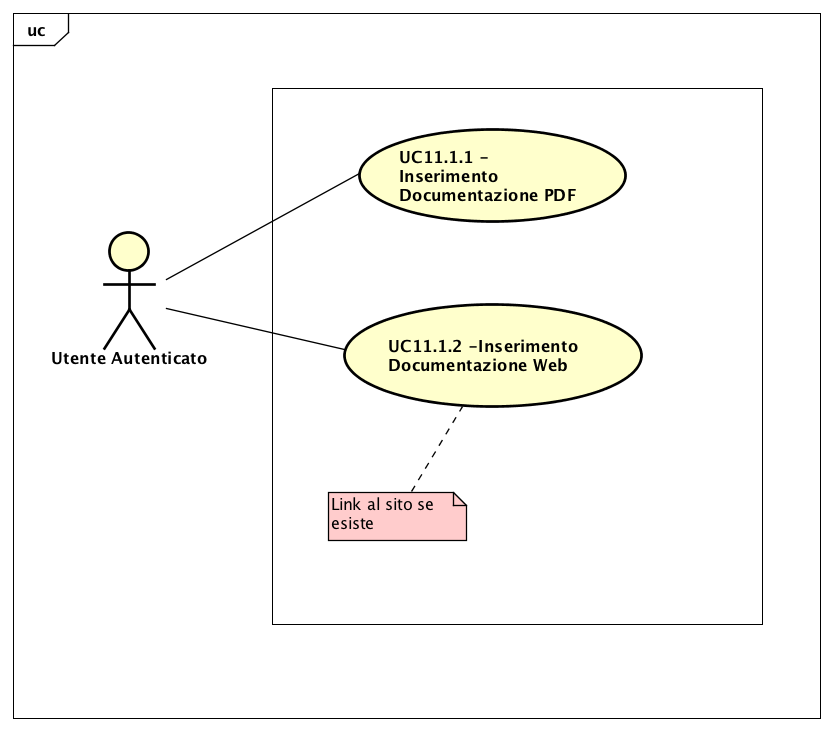
\includegraphics[scale=0.45]{UML/UC11_1.png}
	\caption{Caso d'uso UC11: Registrazione Nuova API}
\end{figure}

\renewcommand*{\arraystretch}{1.6}
\begin{longtable}{ l | p{11cm}}
	\hline
	\rowcolor{Gray}
	\multicolumn{2}{c}{UC11.1: Inserimento Documentazione API} \\
	\hline
	\textbf{Attori} &Utente Autenticato, Amministratore APIMarket \\
	\textbf{Descrizione} & l'attore inserisce la documentazione della propria nuova API \\
	\textbf{Pre-Condizioni} &  l'attore ha scelto di inserire la documentazione della propria nuova API\\
	\textbf{Post-Condizioni}&l'attore ha inserito la documentazione della propria nuova API\\
	\textbf{Scenario Principale} & \begin{enumerate*}[label=(\arabic*.),itemjoin={\newline}]
			\item l'attore può inserire la documentazione della propria nuova API
	\end{enumerate*}\\
\end{longtable}



%\paragraph{Caso d'uso UC11.1.1: Inserimento Documentazione PDF}
\label{UC11.1.1}

\renewcommand*{\arraystretch}{1.6}
\begin{longtable}{ l | p{11cm}}
	\hline
	\rowcolor{Gray}
	\multicolumn{2}{c}{Caso d'uso UC11.1.1: Inserimento Documentazione PDF} \\
	\hline
	\textbf{Attori} &Utente Autenticato, Amministratore APIMarket \\
	\textbf{Descrizione} & l'attore inserisce la documentazione PDF della propria nuova API\\
	\textbf{Pre-Condizioni} &  l'attore ha scelto di inserire la documentazione PDF della propria nuova API\\
	\textbf{Post-Condizioni}&l'attore ha inserito la documentazione PDF della propria nuova API\\
	\textbf{Scenario Principale} & \begin{enumerate*}[label=(\arabic*.),itemjoin={\newline}]
		\item l'attore può inserire la documentazione PDF della propria nuova API
	\end{enumerate*}\\
\end{longtable}



%\subsubsection{Caso d'uso UC11.1.2: Inserimento Documentazione Web}
\label{UC11.1.2}

\renewcommand*{\arraystretch}{1.6}
\begin{longtable}{ l | p{11cm}}
	\hline
	\rowcolor{Gray}
	\multicolumn{2}{c}{UC11.1.2: Inserimento Documentazione Web} \\
	\hline
	\textbf{Attori} &Utente Autenticato, Amministratore APIMarket \\
	\textbf{Descrizione} & l'attore inserisce la documentazione Web della propria nuova API\\
	\textbf{Pre-Condizioni} & 'attore ha scelto di inserire la documentazione Web della propria nuova API\\
	\textbf{Post-Condizioni}&l'attore ha inserito la documentazione Web della propria nuova API\\
	\textbf{Scenario Principale} & \begin{enumerate*}[label=(\arabic*.),itemjoin={\newline}]
		\item l'attore può inserire la documentazione Web della propria nuova API
	\end{enumerate*}\\
\end{longtable}



%\subsubsection{Caso d'uso UC11.2: Registrazione Interfaccia API}
\label{UC11.2}

\renewcommand*{\arraystretch}{1.6}
\begin{longtable}{ l | p{11cm}}
	\hline
	\rowcolor{Gray}
	\multicolumn{2}{c}{UC11.2: Registrazione Interfaccia API} \\
	\hline
	\textbf{Attori} &Utente Autenticato, Amministratore APIMarket \\
	\textbf{Descrizione} & l'attore registra l'interfaccia della propria nuova API \\
	\textbf{Pre-Condizioni} & l'attore ha scelto di registrare l'interfaccia della propria nuova API\\
	\textbf{Post-Condizioni}&l'attore ha registrato l'interfaccia della propria nuova API\\
	\textbf{Scenario Principale} & \begin{enumerate*}[label=(\arabic*.),itemjoin={\newline}]
		\item l'attore può registrare l'interfaccia della propria nuova API
	\end{enumerate*}\\
\end{longtable}




%\subsubsection{Caso d'uso UC11.3: Conferma Registrazione Nuova API}
\label{UC11.3}

\renewcommand*{\arraystretch}{1.6}
\begin{longtable}{ l | p{11cm}}
	\hline
	\rowcolor{Gray}
	\multicolumn{2}{c}{UC11.3: Conferma Registrazione Nuova API} \\
	\hline
	\textbf{Attori} &Utente Autenticato, Amministratore APIMarket \\
	\textbf{Descrizione} & l'attore conferma la registrazione della propria nuova API \\
	\textbf{Pre-Condizioni} & l'attore ha scelto di confermare la registrazione della propria nuova API\\
	\textbf{Post-Condizioni}&l'attore ha confermato la registrazione della propria nuova API\\
	\textbf{Scenario Principale} & \begin{enumerate*}[label=(\arabic*.),itemjoin={\newline}]
		\item l'attore può confermare la registrazione della propria nuova API
	\end{enumerate*}\\
\end{longtable}



%\subsubsection{Caso d'uso UC11.4: Visualizzazione Errore Registrazione Nuova API}
\label{UC11.4}

\renewcommand*{\arraystretch}{1.6}
\begin{longtable}{ l | p{11cm}}
	\hline
	\rowcolor{Gray}
	\multicolumn{2}{c}{UC11.4: Visualizzazione Errore Registrazione Nuova API} \\
	\hline
	\textbf{Attori} &Utente Autenticato, Amministratore APIMarket \\
	\textbf{Descrizione} &  l'attore visualizza l'errore nella registrazione della propria nuova API \\
	\textbf{Pre-Condizioni} & l'attore ha scelto di visualizzare l'errore nella registrazione della propria nuova API;\\
	\textbf{Post-Condizioni}&l'attore ha visualizzato l'errore nella registrazione della propria nuova API\\
	\textbf{Scenario Principale} & \begin{enumerate*}[label=(\arabic*.),itemjoin={\newline}]
		\item l'attore può visualizzare l'errore nella registrazione della propria nuova API
	\end{enumerate*}\\
\end{longtable}

\newpage
\subsection{Caso d'uso UC12: Gestione proprio profilo utente}
\label{UC12}
\begin{figure}[ht]
	\centering
	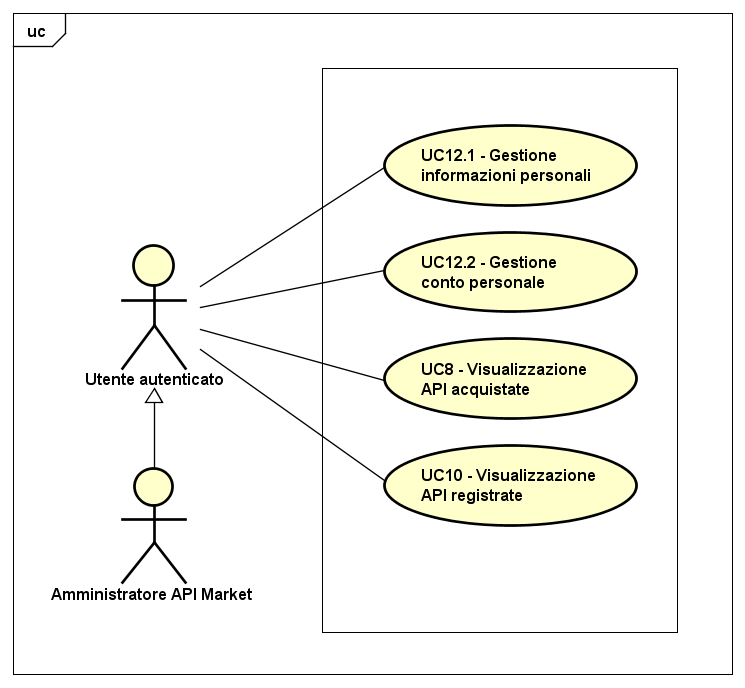
\includegraphics[scale=0.45]{UML/UC12.png}
	\caption{UC12 - Gestione proprio profilo utente}
\end{figure}

\begin{longtable}{ l | p{11cm}}
	\hline
	\rowcolor{Gray}
	\multicolumn{2}{c}{UC12 - Gestione proprio profilo utente} \\
	\hline
	\textbf{Attori} & Cliente, Sviluppatore \\
	\textbf{Descrizione} & L'attore visualizza e/o gestisce le informazioni del proprio profilo utente \\
	\textbf{Pre-Condizioni} & L'attore si trova nella schermata relativa alla gestione del proprio profilo utente \\
	\textbf{Post-Condizioni} & L'attore ha visualizzato e/o gestito le informazioni del proprio profilo utente \\
	\textbf{Scenario Principale} & 
	\begin{enumerate*}[label=(\arabic*.),itemjoin={\newline}]
		\item L'attore può gestire le proprie informazioni personali (UC12.1)
		\item L'attore può gestire il proprio conto utente (UC12.2)
		\item L'attore può visualizzare le API da lui acquistate (UC8)
		\item Lo sviluppatore può visualizzare le API da lui registrate (UC10)
	\end{enumerate*}\\
\end{longtable}

\newpage
\subsubsection{Caso d'uso UC12.1: Gestione informazioni personali}
\label{UC12_1}
\begin{figure}[ht]
	\centering
	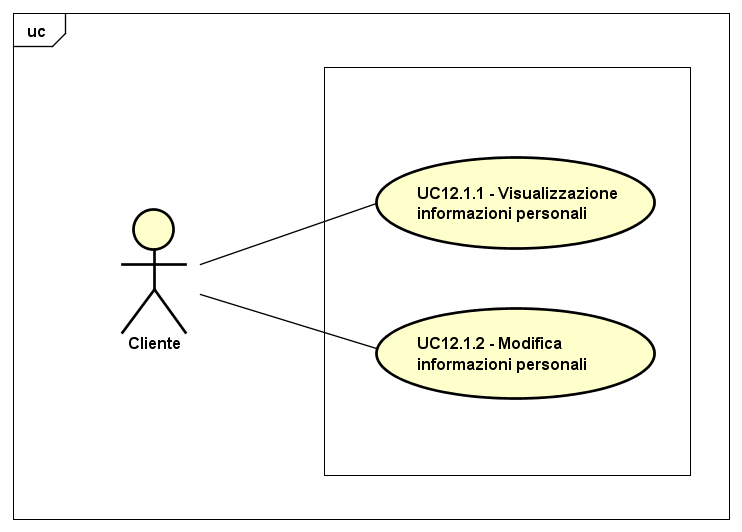
\includegraphics[scale=0.45]{UML/UC12_1.png}
	\caption{UC12.1: Gestione informazioni personali}
\end{figure}

\begin{minipage}{\linewidth}
	\begin{tabular}{ l | p{11cm}}
		\hline
		\rowcolor{Gray}
		\multicolumn{2}{c}{UC12.1 - Gestione informazioni personali} \\
		\hline
		\textbf{Attori} & Cliente \\
		\textbf{Descrizione} & L'attore visualizza e/o modifica le proprie informazioni personali \\
		\textbf{Pre-Condizioni} & L'attore si trova nella schermata relativa alla gestione del proprio profilo utente \\
		\textbf{Post-Condizioni} & L'attore ha visualizzato e/o modificato le proprie informazioni personali \\
		\textbf{Scenario Principale} & 
		\begin{enumerate*}[label=(\arabic*.),itemjoin={\newline}]
			\item L'attore può visualizzare le proprie informazioni personali (UC12.1.1)
			\item L'attore può modificare le proprie informazioni personali (UC12.1.2)
		\end{enumerate*}
	\end{tabular}
\end{minipage}

\newpage
\paragraph{Caso d'uso UC12.1.1: Visualizzazione informazioni personali}
\label{UC12_1_1}
\begin{figure}[ht]
	\centering
	\includegraphics[scale=0.45]{UML/UC12_1_1.png}
	\caption{UC12.1.1: Visualizzazione informazioni personali}
\end{figure}

\begin{minipage}{\linewidth}
\begin{tabular}{ l | p{11cm}}
	\hline
	\rowcolor{Gray}
	\multicolumn{2}{c}{UC12.1.1 - Visualizzazione informazioni personali} \\
	\hline
	\textbf{Attori} & Cliente \\
	\textbf{Descrizione} & L'attore visualizza le proprie informazioni personali \\
	\textbf{Pre-Condizioni} & L'attore si trova nella schermata relativa alla gestione del proprio profilo utente \\
	\textbf{Post-Condizioni} & L'attore ha visualizzato le proprie informazioni personali \\
	\textbf{Scenario Principale} & 
	\begin{enumerate*}[label=(\arabic*.),itemjoin={\newline}]
		\item L'attore può visualizzare il proprio nome (UC12.1.1.1)
		\item L'attore può visualizzare il proprio cognome (UC12.1.1.2)
		\item L'attore può visualizzare il proprio username (UC12.1.1.3)
		\item L'attore può visualizzare la propria email (UC12.1.1.4)
		\item L'attore può visualizzare il proprio avatar (UC12.1.1.5)
		\item L'attore può visualizzare la tipologia del proprio account (UC12.1.1.6)
	\end{enumerate*}\\
\end{tabular}
\end{minipage}

\subparagraph{Caso d'uso UC12.1.1.1: Visualizzazione nome}
\label{UC12_1_1_1}

\begin{minipage}{\linewidth}
\begin{tabular}{ l | p{11cm}}
	\hline
	\rowcolor{Gray}
	\multicolumn{2}{c}{UC12.1.1.1 - Visualizzazione nome} \\
	\hline
	\textbf{Attori} & Cliente \\
	\textbf{Descrizione} & L'attore visualizzare il proprio nome \\
	\textbf{Pre-Condizioni} & L'attore si trova nella schermata relativa alla gestione delle informazioni personali \\
	\textbf{Post-Condizioni} & L'attore ha visualizzato il proprio nome \\
	\textbf{Scenario Principale} & 
	\begin{enumerate*}[label=(\arabic*.),itemjoin={\newline}]
		\item L'attore può visualizzare il proprio nome
	\end{enumerate*}
\end{tabular}
\end{minipage}

\subparagraph{Caso d'uso UC12.1.1.2: Visualizzazione cognome}
\label{UC12_1_1_2}

\begin{minipage}{\linewidth}
	\begin{tabular}{ l | p{11cm}}
		\hline
		\rowcolor{Gray}
		\multicolumn{2}{c}{UC12.1.1.2 - Visualizzazione cognome} \\
		\hline
		\textbf{Attori} & Cliente \\
		\textbf{Descrizione} & L'attore visualizzare il proprio cognome \\
	\textbf{Pre-Condizioni} & L'attore si trova nella schermata relativa alla gestione delle informazioni personali \\
	\textbf{Post-Condizioni} & L'attore ha visualizzato il proprio cognome \\
	\textbf{Scenario Principale} & 
	\begin{enumerate*}[label=(\arabic*.),itemjoin={\newline}]
		\item L'attore può visualizzare il proprio cognome
	\end{enumerate*}
	\end{tabular}
\end{minipage}

\subparagraph{Caso d'uso UC12.1.1.3: Visualizzazione username}
\label{UC12_1_1_3}

\begin{minipage}{\linewidth}
	\begin{tabular}{ l | p{11cm}}
		\hline
		\rowcolor{Gray}
		\multicolumn{2}{c}{UC12.1.1.3 - Visualizzazione username} \\
		\hline
		\textbf{Attori} & Cliente \\
		\textbf{Descrizione} & L'attore visualizzare il proprio username \\
	\textbf{Pre-Condizioni} & L'attore si trova nella schermata relativa alla gestione delle informazioni personali \\
	\textbf{Post-Condizioni} & L'attore ha visualizzato il proprio username \\
	\textbf{Scenario Principale} & 
	\begin{enumerate*}[label=(\arabic*.),itemjoin={\newline}]
		\item L'attore può visualizzare il proprio username
	\end{enumerate*}
	\end{tabular}
\end{minipage}

\subparagraph{Caso d'uso UC12.1.1.4: Visualizzazione email}
\label{UC12_1_1_4}

\begin{minipage}{\linewidth}
	\begin{tabular}{ l | p{11cm}}
		\hline
		\rowcolor{Gray}
		\multicolumn{2}{c}{UC12.1.1.4 - Visualizzazione email} \\
		\hline
		\textbf{Attori} & Cliente \\
		\textbf{Descrizione} & L'attore visualizzare la propria email \\
		\textbf{Pre-Condizioni} & L'attore si trova nella schermata relativa alla gestione delle informazioni personali \\
		\textbf{Post-Condizioni} & L'attore ha visualizzato la propria email \\
		\textbf{Scenario Principale} & 
		\begin{enumerate*}[label=(\arabic*.),itemjoin={\newline}]
			\item L'attore può visualizzare la propria email
		\end{enumerate*}
	\end{tabular}
\end{minipage}

\subparagraph{Caso d'uso UC12.1.1.5: Visualizzazione avatar}
\label{UC12_1_1_5}

\begin{minipage}{\linewidth}
	\begin{tabular}{ l | p{11cm}}
		\hline
		\rowcolor{Gray}
		\multicolumn{2}{c}{UC12.1.1.5 - Visualizzazione avatar} \\
		\hline
		\textbf{Attori} & Cliente \\
		\textbf{Descrizione} & L'attore visualizzare il proprio avatar \\
		\textbf{Pre-Condizioni} & L'attore si trova nella schermata relativa alla gestione delle informazioni personali \\
		\textbf{Post-Condizioni} & L'attore ha visualizzato il proprio avatar \\
		\textbf{Scenario Principale} & 
		\begin{enumerate*}[label=(\arabic*.),itemjoin={\newline}]
			\item L'attore può visualizzare il proprio avatar
		\end{enumerate*}
	\end{tabular}
\end{minipage}

\subparagraph{Caso d'uso UC12.1.1.6: Visualizzazione tipologia account}
\label{UC12_1_1_6}

\begin{minipage}{\linewidth}
	\begin{tabular}{ l | p{11cm}}
		\hline
		\rowcolor{Gray}
		\multicolumn{2}{c}{UC12.1.1.6 - Visualizzazione tipologia account} \\
		\hline
		\textbf{Attori} & Cliente \\
		\textbf{Descrizione} & L'attore visualizzare la tipologia del proprio account \\
		\textbf{Pre-Condizioni} & L'attore si trova nella schermata relativa alla gestione delle informazioni personali \\
		\textbf{Post-Condizioni} & L'attore ha visualizzato la tipologia del proprio account \\
		\textbf{Scenario Principale} & 
		\begin{enumerate*}[label=(\arabic*.),itemjoin={\newline}]
			\item L'attore può visualizzare la tipologia del proprio account
		\end{enumerate*}
	\end{tabular}
\end{minipage}

\newpage
\paragraph{Caso d'uso UC12.1.2: Modifica informazioni personali}
\label{UC12_1_2}
\begin{figure}[ht]
	\centering
	\includegraphics[scale=0.45]{UML/UC12_1_2.png}
	\caption{UC12.1.2: Modifica informazioni personali}
\end{figure}

\begin{tabular}{ l | p{11cm}}
	\hline
	\rowcolor{Gray}
	\multicolumn{2}{c}{UC12.1.2 - Modifica informazioni personali} \\
	\hline
	\textbf{Attori} & Cliente \\
	\textbf{Descrizione} & L'attore modifica le proprie informazioni personali \\
	\textbf{Pre-Condizioni} & L'attore si trova nella schermata relativa alla gestione del proprio profilo utente \\
	\textbf{Post-Condizioni} & L'attore ha modificato le proprie informazioni personali \\
	\textbf{Scenario Principale} & 
	\begin{enumerate*}[label=(\arabic*.),itemjoin={\newline}]
		\item L'attore può modificare il proprio nome (UC12.1.2.1)
		\item L'attore può modificare il proprio cognome (UC12.1.2.2)
		\item L'attore può modificare il proprio username (UC12.1.2.3)
		\item L'attore può modificare la propria email (UC12.1.2.4)
		\item L'attore può modificare la propria password (UC12.1.2.5)
		\item L'attore può modificare il proprio avatar (UC12.1.2.6)
		\item L'attore può confermare la modifica alle proprie informazioni personali (UC12.1.2.7)
		\item L'attore può migliorare il proprio status a sviluppatore (UC12.1.2.9)
	\end{enumerate*}\\
	\textbf{Scenari Alternativi} & 
	\begin{enumerate*}[label=(\arabic*.),itemjoin={\newline}]
		\item L'attore, dopo aver confermato le modifiche alle proprie informazioni personali, può visualizzare un messaggio di errore informativo (E.g: dati non validi, formati dei file errati), e le modifiche non avvengono (UC12.1.2.8)
	\end{enumerate*}\\
\end{tabular}

\subparagraph{Caso d'uso UC12.1.2.1: Modifica nome}
\label{UC12_1_2_1}

\begin{minipage}{\linewidth}
	\begin{tabular}{ l | p{11cm}}
		\hline
		\rowcolor{Gray}
		\multicolumn{2}{c}{UC12.1.2.1 - Modifica nome} \\
		\hline
		\textbf{Attori} & Cliente \\
		\textbf{Descrizione} & L'attore modifica il proprio nome \\
		\textbf{Pre-Condizioni} & L'attore si trova nella schermata relativa alla gestione delle informazioni personali \\
		\textbf{Post-Condizioni} & L'attore ha modificato il proprio nome \\
		\textbf{Scenario Principale} & 
		\begin{enumerate*}[label=(\arabic*.),itemjoin={\newline}]
			\item L'attore può modificare il proprio nome
		\end{enumerate*}
	\end{tabular}
\end{minipage}

\subparagraph{Caso d'uso UC12.1.2.2: Modifica cognome}
\label{UC12_1_2_2}

\begin{minipage}{\linewidth}
	\begin{tabular}{ l | p{11cm}}
		\hline
		\rowcolor{Gray}
		\multicolumn{2}{c}{UC12.1.2.2 - Modifica cognome} \\
		\hline
		\textbf{Attori} & Cliente \\
		\textbf{Descrizione} & L'attore modifica il proprio cognome \\
		\textbf{Pre-Condizioni} & L'attore si trova nella schermata relativa alla gestione delle informazioni personali \\
		\textbf{Post-Condizioni} & L'attore ha modificato il proprio cognome \\
		\textbf{Scenario Principale} & 
		\begin{enumerate*}[label=(\arabic*.),itemjoin={\newline}]
			\item L'attore può modificare il proprio cognome
		\end{enumerate*}
	\end{tabular}
\end{minipage}

\subparagraph{Caso d'uso UC12.1.2.3: Modifica username}
\label{UC12_1_2_3}

\begin{minipage}{\linewidth}
	\begin{tabular}{ l | p{11cm}}
		\hline
		\rowcolor{Gray}
		\multicolumn{2}{c}{UC12.1.2.3 - Modifica username} \\
		\hline
		\textbf{Attori} & Cliente \\
		\textbf{Descrizione} & L'attore modifica il proprio username \\
		\textbf{Pre-Condizioni} & L'attore si trova nella schermata relativa alla gestione delle informazioni personali \\
		\textbf{Post-Condizioni} & L'attore ha modificato il proprio username \\
		\textbf{Scenario Principale} & 
		\begin{enumerate*}[label=(\arabic*.),itemjoin={\newline}]
			\item L'attore può modificare il proprio username
		\end{enumerate*}
	\end{tabular}
\end{minipage}

\subparagraph{Caso d'uso UC12.1.2.4: Modifica email}
\label{UC12_1_2_4}

\begin{minipage}{\linewidth}
	\begin{tabular}{ l | p{11cm}}
		\hline
		\rowcolor{Gray}
		\multicolumn{2}{c}{UC12.1.2.4 - Modifica email} \\
		\hline
		\textbf{Attori} & Cliente \\
		\textbf{Descrizione} & L'attore modifica la propria email \\
		\textbf{Pre-Condizioni} & L'attore si trova nella schermata relativa alla gestione delle informazioni personali \\
		\textbf{Post-Condizioni} & L'attore ha modificato la propria email \\
		\textbf{Scenario Principale} & 
		\begin{enumerate*}[label=(\arabic*.),itemjoin={\newline}]
			\item L'attore può modificare la propria email
		\end{enumerate*}
	\end{tabular}
\end{minipage}

\subparagraph{Caso d'uso UC12.1.2.5: Modifica password}
\label{UC12_1_2_5}

\begin{minipage}{\linewidth}
	\begin{tabular}{ l | p{11cm}}
		\hline
		\rowcolor{Gray}
		\multicolumn{2}{c}{UC12.1.2.5 - Modifica password} \\
		\hline
		\textbf{Attori} & Cliente \\
		\textbf{Descrizione} & L'attore modifica la propria password \\
		\textbf{Pre-Condizioni} & L'attore si trova nella schermata relativa alla gestione delle informazioni personali \\
		\textbf{Post-Condizioni} & L'attore ha modificato la propria password \\
		\textbf{Scenario Principale} & 
		\begin{enumerate*}[label=(\arabic*.),itemjoin={\newline}]
			\item L'attore può modificare la propria password
		\end{enumerate*}
	\end{tabular}
\end{minipage}

\subparagraph{Caso d'uso UC12.1.2.6: Modifica avatar}
\label{UC12_1_2_6}

\begin{minipage}{\linewidth}
	\begin{tabular}{ l | p{11cm}}
		\hline
		\rowcolor{Gray}
		\multicolumn{2}{c}{UC12.1.2.6 - Modifica avatar} \\
		\hline
		\textbf{Attori} & Cliente \\
		\textbf{Descrizione} & L'attore modifica il proprio avatar \\
		\textbf{Pre-Condizioni} & L'attore si trova nella schermata relativa alla gestione delle informazioni personali \\
		\textbf{Post-Condizioni} & L'attore ha modificato il proprio avatar \\
		\textbf{Scenario Principale} & 
		\begin{enumerate*}[label=(\arabic*.),itemjoin={\newline}]
			\item L'attore può modificare il proprio avatar
		\end{enumerate*}
	\end{tabular}
\end{minipage}

\subparagraph{Caso d'uso UC12.1.2.6: Modifica avatar}
\label{UC12_1_2_6}

\begin{minipage}{\linewidth}
	\begin{tabular}{ l | p{11cm}}
		\hline
		\rowcolor{Gray}
		\multicolumn{2}{c}{UC12.1.2.6 - Modifica avatar} \\
		\hline
		\textbf{Attori} & Cliente \\
		\textbf{Descrizione} & L'attore modifica il proprio avatar \\
		\textbf{Pre-Condizioni} & L'attore si trova nella schermata relativa alla gestione delle informazioni personali \\
		\textbf{Post-Condizioni} & L'attore ha modificato il proprio avatar \\
		\textbf{Scenario Principale} & 
		\begin{enumerate*}[label=(\arabic*.),itemjoin={\newline}]
			\item L'attore può modificare il proprio avatar
		\end{enumerate*}
	\end{tabular}
\end{minipage}

\subparagraph{Caso d'uso UC12.1.2.7: Conferma modifica informazioni personali}
\label{UC12_1_2_7}

\begin{minipage}{\linewidth}
	\begin{tabular}{ l | p{11cm}}
		\hline
		\rowcolor{Gray}
		\multicolumn{2}{c}{UC12.1.2.7 - Conferma modifica informazioni personali} \\
		\hline
		\textbf{Attori} & Cliente \\
		\textbf{Descrizione} & L'attore conferma la modifica delle informazioni personali \\
		\textbf{Pre-Condizioni} & L'attore si trova nella schermata relativa alla gestione delle informazioni personali \\
		\textbf{Post-Condizioni} & L'attore ha confermato la modifica delle informazioni personali \\
		\textbf{Scenario Principale} & 
		\begin{enumerate*}[label=(\arabic*.),itemjoin={\newline}]
			\item L'attore può confermare la modifica delle informazioni personali, visualizzando un messaggio di successo
		\end{enumerate*}\\
	\end{tabular}
\end{minipage}

\subparagraph{Caso d'uso UC12.1.2.8: Errore modifica informazioni personali}
\label{UC12_1_2_8}

\begin{minipage}{\linewidth}
	\begin{tabular}{ l | p{11cm}}
		\hline
		\rowcolor{Gray}
		\multicolumn{2}{c}{UC12.1.2.8 - Errore modifica informazioni personali} \\
		\hline
		\textbf{Attori} & Cliente \\
		\textbf{Descrizione} & L'attore visualizza un messaggio di errore informativo e la modifica delle informazioni personali non avviene \\
		\textbf{Pre-Condizioni} & L'attore ha confermato la modifica delle informazioni personali ma si è verificato un errore \\
		\textbf{Post-Condizioni} & L'attore ha visualizzato un messaggio di errore informativo \\
		\textbf{Scenario Principale} & 
		\begin{enumerate*}[label=(\arabic*.),itemjoin={\newline}]
			\item L'attore può visualizzare un messaggio di errore informativo e la modifica delle informazioni personali non avviene
		\end{enumerate*}\\
	\end{tabular}
\end{minipage}

\subparagraph{Caso d'uso UC12.1.2.9: Upgrade a sviluppatore}
\label{UC12_1_2_9}

\begin{minipage}{\linewidth}
	\begin{tabular}{ l | p{11cm}}
		\hline
		\rowcolor{Gray}
		\multicolumn{2}{c}{UC12.1.2.9 - Upgrade a sviluppatore} \\
		\hline
		\textbf{Attori} & Cliente \\
		\textbf{Descrizione} & Il cliente base migliora il proprio status diventando sviluppatore \\
		\textbf{Pre-Condizioni} & Il cliente base si trova nella schermata relativa alla gestione delle informazioni personali \\
		\textbf{Post-Condizioni} & Il cliente base ha migliorato il proprio status diventando sviluppatore \\
		\textbf{Scenario Principale} & 
		\begin{enumerate*}[label=(\arabic*.),itemjoin={\newline}]
			\item Il cliente base può migliorare il proprio status diventando sviluppatore
		\end{enumerate*}
	\end{tabular}
\end{minipage}

\newpage
\subsubsection{Caso d'uso UC12.2: Gestione conto personale}
\label{UC12_2}
\begin{figure}[ht]
	\centering
	\includegraphics[scale=0.45]{UML/UC12_2.png}
	\caption{UC12.2: Gestione conto personale}
\end{figure}

\begin{minipage}{\linewidth}
	\begin{tabular}{ l | p{11cm}}
		\hline
		\rowcolor{Gray}
		\multicolumn{2}{c}{UC12.2 - Gestione conto personale} \\
		\hline
		\textbf{Attori} & Cliente \\
		\textbf{Descrizione} & L'attore visualizza le informazioni del proprio conto utente e/o effettua una ricarica su di esso \\
		\textbf{Pre-Condizioni} & L'attore si trova nella schermata relativa alla gestione del proprio profilo utente \\
		\textbf{Post-Condizioni} & L'attore ha visualizzato il saldo del proprio conto utente e/o effettuato una ricarica su di esso \\
		\textbf{Scenario Principale} & 
		\begin{enumerate*}[label=(\arabic*.),itemjoin={\newline}]
			\item L'attore può visualizzare il saldo corrente del proprio conto utente (UC12.2.1)
			\item L'attore può effettuare una ricarica sul proprio conto utente (UC12.2.2)
		\end{enumerate*}
	\end{tabular}
\end{minipage}

\paragraph{Caso d'uso UC12.2.1: Visualizzazione saldo conto}
\label{UC12_2_1}

\begin{minipage}{\linewidth}
	\begin{tabular}{ l | p{11cm}}
		\hline
		\rowcolor{Gray}
		\multicolumn{2}{c}{UC12.2.1 - Visualizzazione saldo conto} \\
		\hline
		\textbf{Attori} & Cliente \\
		\textbf{Descrizione} & L'attore visualizza il saldo corrente del proprio conto utente \\
		\textbf{Pre-Condizioni} & L'attore si trova nella schermata relativa alla gestione del proprio conto utente \\
		\textbf{Post-Condizioni} & L'attore ha visualizzato il saldo corrente del proprio conto utente \\
		\textbf{Scenario Principale} & 
		\begin{enumerate*}[label=(\arabic*.),itemjoin={\newline}]
			\item L'attore può visualizzare il saldo corrente del proprio conto utente
		\end{enumerate*}\\
	\end{tabular}
\end{minipage}

\paragraph{Caso d'uso UC12.2.2: Ricarica conto}
\label{UC12_2_2}
\begin{figure}[ht]
	\centering
	\includegraphics[scale=0.45]{UML/UC12_2_2.png}
	\caption{UC12.2.2: Ricarica conto}
\end{figure}

\begin{minipage}{\linewidth}
	\begin{tabular}{ l | p{11cm}}
		\hline
		\rowcolor{Gray}
		\multicolumn{2}{c}{UC12.2.2 - Ricarica conto} \\
		\hline
		\textbf{Attori} & Cliente, PayPal \\
		\textbf{Descrizione} & L'attore effettua una ricarica sul proprio conto utente \\
		\textbf{Pre-Condizioni} & L'attore si trova nella schermata relativa alla gestione del proprio conto utente \\
		\textbf{Post-Condizioni} & L'attore ha effettuato una ricarica sul proprio conto utente \\
		\textbf{Scenario Principale} & 
		\begin{enumerate*}[label=(\arabic*.),itemjoin={\newline}]
			\item L'attore può effettuare una ricarica tramite PayPal sul proprio conto utente (UC12.2.2.1)
		\end{enumerate*}\\
		\textbf{Scenari Alternativi} & 
		\begin{enumerate*}[label=(\arabic*.),itemjoin={\newline}]
			\item L'attore può visualizzare un messaggio di errore informativo (E.g: dati errati), e la ricarica tramite PayPal sul proprio conto utente non avviene (UC12.2.2.2)
		\end{enumerate*}\\
	\end{tabular}
\end{minipage}

\subparagraph{Caso d'uso UC12.2.2.1: Ricarica tramite PayPal}
\label{UC12_2_2_1}

\begin{minipage}{\linewidth}
	\begin{tabular}{ l | p{11cm}}
		\hline
		\rowcolor{Gray}
		\multicolumn{2}{c}{UC12.2.2.1 - Ricarica tramite PayPal} \\
		\hline
		\textbf{Attori} & Cliente, PayPal \\
		\textbf{Descrizione} & L'attore effettua una ricarica tramite PayPal sul proprio conto utente \\
		\textbf{Pre-Condizioni} & L'attore si trova nella schermata relativa alla ricarica del proprio conto utente \\
		\textbf{Post-Condizioni} & L'attore ha effettuato una ricarica tramite PayPal sul proprio conto utente \\
		\textbf{Scenario Principale} & 
		\begin{enumerate*}[label=(\arabic*.),itemjoin={\newline}]
			\item L'attore può effettuare una ricarica tramite PayPal sul proprio conto utente
		\end{enumerate*}\\
	\end{tabular}
\end{minipage}

\subparagraph{Caso d'uso UC12.2.2.2: Errore ricarica PayPal}
\label{UC12_2_2_2}

\begin{minipage}{\linewidth}
	\begin{tabular}{ l | p{11cm}}
		\hline
		\rowcolor{Gray}
		\multicolumn{2}{c}{UC12.2.2.2 - Errore ricarica PayPal} \\
		\hline
		\textbf{Attori} & Cliente, PayPal \\
		\textbf{Descrizione} & L'attore visualizza un messaggio di errore informativo e la ricarica tramite PayPal sul proprio conto utente non avviene \\
		\textbf{Pre-Condizioni} & L'attore ha confermato la ricarica tramite PayPal sul proprio conto utente ma si è verificato un errore \\
		\textbf{Post-Condizioni} & L'attore ha visualizzato un messaggio di errore informativo \\
		\textbf{Scenario Principale} & 
		\begin{enumerate*}[label=(\arabic*.),itemjoin={\newline}]
			\item L'attore può visualizzare un messaggio di errore informativo e la ricarica tramite PayPal sul proprio conto utente non avviene
		\end{enumerate*}\\
	\end{tabular}
\end{minipage}

\newpage
\subsubsection{Caso d'uso UC12.3: Visualizzazione storico transazioni}
\label{UC12_3}
\begin{figure}[ht]
	\centering
	\includegraphics[scale=0.45]{UML/UC12_3.png}
	\caption{UC12.3: Visualizzazione storico transazioni}
\end{figure}

\begin{minipage}{\linewidth}
	\begin{tabular}{ l | p{11cm}}
		\hline
		\rowcolor{Gray}
		\multicolumn{2}{c}{UC12.3 - Visualizzazione storico transazioni} \\
		\hline
		\textbf{Attori} & Cliente, Sviluppatore \\
		\textbf{Descrizione} & L'attore visualizza lo storico delle proprie transazioni \\
		\textbf{Pre-Condizioni} & L'attore si trova nella schermata relativa alla gestione del proprio profilo utente \\
		\textbf{Post-Condizioni} & L'attore ha visualizzato lo storico delle proprie transazioni \\
		\textbf{Scenario Principale} & 
		\begin{enumerate*}[label=(\arabic*.),itemjoin={\newline}]
			\item L'attore può scegliere i filtri di visualizzazione (UC12.3.1)
			\item L'attore può visualizzare la lista delle proprie transazioni concluse (UC12.3.2)
			\item Lo sviluppatore può visualizzare la lista dei propri crediti (UC12.3.3)
		\end{enumerate*}
	\end{tabular}
\end{minipage}

\newpage
\paragraph{Caso d'uso UC12.3.1: Scelta filtri storico transazioni}
\label{UC12_3_1}
\begin{figure}[ht]
	\centering
	\includegraphics[scale=0.45]{UML/UC12_3_1.png}
	\caption{UC12.3.1: Scelta filtri storico transazioni}
\end{figure}

\begin{minipage}{\linewidth}
	\begin{tabular}{ l | p{11cm}}
		\hline
		\rowcolor{Gray}
		\multicolumn{2}{c}{UC12.3.1 - Scelta filtri storico transazioni} \\
		\hline
		\textbf{Attori} & Cliente \\
		\textbf{Descrizione} & L'attore scegliere i filtri per lo storico delle proprie transazioni \\
	\textbf{Pre-Condizioni} & L'attore si trova nella schermata relativa alla visualizzazione dello storico delle proprie transazioni \\
	\textbf{Post-Condizioni} & L'attore ha scelto i filtri per lo storico delle proprie transazioni \\
	\textbf{Scenario Principale} & 
	\begin{enumerate*}[label=(\arabic*.),itemjoin={\newline}]
		\item L'attore può scegliere il filtro per ordine cronologico (UC12.3.1.1)
		\item L'attore può scegliere il filtro per tipologia di transazione (UC12.3.1.2)
	\end{enumerate*}
	\end{tabular}
\end{minipage}

\subparagraph{Caso d'uso UC12.3.1.1: Scelta filtro per ordine cronologico}
\label{UC12_3_1_1}

\begin{minipage}{\linewidth}
	\begin{tabular}{ l | p{11cm}}
		\hline
		\rowcolor{Gray}
		\multicolumn{2}{c}{UC12.3.1.1 - Scelta filtro per ordine cronologico} \\
		\hline
		\textbf{Attori} & Cliente \\
		\textbf{Descrizione} & L'attore sceglie il filtro per ordine cronologico \\
	\textbf{Pre-Condizioni} & L'attore si trova nella schermata relativa alla visualizzazione dello storico delle proprie transazioni \\
	\textbf{Post-Condizioni} & L'attore ha scelto il filtro per ordine cronologico \\
	\textbf{Scenario Principale} & 
	\begin{enumerate*}[label=(\arabic*.),itemjoin={\newline}]
		\item L'attore può scegliere il filtro per ordine cronologico
	\end{enumerate*}
	\end{tabular}
\end{minipage}

\subparagraph{Caso d'uso UC12.3.1.2: Scelta filtro per tipologia di transazione}
\label{UC12_3_1_2}

\begin{minipage}{\linewidth}
	\begin{tabular}{ l | p{11cm}}
		\hline
		\rowcolor{Gray}
		\multicolumn{2}{c}{UC12.3.1.2 - Scelta filtro per tipologia di transazione} \\
		\hline
		\textbf{Attori} & Cliente \\
		\textbf{Descrizione} & L'attore sceglie il filtro per tipologia di transazione \\
	\textbf{Pre-Condizioni} & L'attore si trova nella schermata relativa alla visualizzazione dello storico delle proprie transazioni \\
	\textbf{Post-Condizioni} & L'attore ha scelto il filtro per tipologia di transazione \\
	\textbf{Scenario Principale} & 
	\begin{enumerate*}[label=(\arabic*.),itemjoin={\newline}]
		\item L'attore può scegliere il filtro per tipologia di transazione
	\end{enumerate*}
	\end{tabular}
\end{minipage}

\newpage
\paragraph{Caso d'uso UC12.3.2: Visualizzazione lista transazioni concluse}
\label{UC12_3_2}
\begin{figure}[ht]
	\centering
	\includegraphics[scale=0.45]{UML/UC12_3_2.png}
	\caption{UC12.3.2: Visualizzazione lista transazioni concluse}
\end{figure}

\begin{minipage}{\linewidth}
	\begin{tabular}{ l | p{11cm}}
		\hline
		\rowcolor{Gray}
		\multicolumn{2}{c}{UC12.3.2 - Visualizzazione lista transazioni concluse} \\
		\hline
		\textbf{Attori} & Cliente \\
		\textbf{Descrizione} & L'attore visualizza la lista delle proprie transazioni \\
		\textbf{Pre-Condizioni} & L'attore si trova nella schermata relativa alla visualizzazione dello storico delle proprie transazioni \\
		\textbf{Post-Condizioni} & L'attore ha visualizzato la lista delle proprie transazioni \\
		\textbf{Scenario Principale} & 
		\begin{enumerate*}[label=(\arabic*.),itemjoin={\newline}]
			\item L'attore può visualizzare il codice della transazione (UC12.3.2.1)
			\item L'attore può visualizzare l'API di riferimento alla transazione (UC12.3.2.2)
			\item L'attore può visualizzare la tipologia della transazione (UC12.3.2.3)
			\item L'attore può visualizzare l'ammontare del denaro coinvolto nella transazione (UC12.3.2.4)
			\item L'attore può visualizzare la data della transazione (UC12.3.2.5)
		\end{enumerate*}\\
	\end{tabular}
\end{minipage}

\subparagraph{Caso d'uso UC12.3.2.1: Visualizzazione codice transazione}
\label{UC12_3_2_1}

\begin{minipage}{\linewidth}
	\begin{tabular}{ l | p{11cm}}
		\hline
		\rowcolor{Gray}
		\multicolumn{2}{c}{UC12.3.2.1 - Visualizzazione codice transazione} \\
		\hline
		\textbf{Attori} & Cliente \\
		\textbf{Descrizione} & L'attore visualizza il codice della propria transazione \\
	\textbf{Pre-Condizioni} & L'attore si trova nella schermata relativa alla visualizzazione dello storico delle proprie transazioni \\
	\textbf{Post-Condizioni} & L'attore ha visualizzato il codice della propria transazione \\
	\textbf{Scenario Principale} & 
	\begin{enumerate*}[label=(\arabic*.),itemjoin={\newline}]
		\item L'attore può visualizzare il codice della propria transazione
	\end{enumerate*}
	\end{tabular}
\end{minipage}

\subparagraph{Caso d'uso UC12.3.2.2: Visualizzazione API transazione}
\label{UC12_3_2_2}

\begin{minipage}{\linewidth}
	\begin{tabular}{ l | p{11cm}}
		\hline
		\rowcolor{Gray}
		\multicolumn{2}{c}{UC12.3.2.2 - Visualizzazione API transazione} \\
		\hline
		\textbf{Attori} & Cliente \\
		\textbf{Descrizione} & L'attore visualizza l'API di riferimento alla propria transazione \\
	\textbf{Pre-Condizioni} & L'attore si trova nella schermata relativa alla visualizzazione dello storico delle proprie transazioni \\
	\textbf{Post-Condizioni} & L'attore ha visualizzato l'API di riferimento alla propria transazione \\
	\textbf{Scenario Principale} & 
	\begin{enumerate*}[label=(\arabic*.),itemjoin={\newline}]
		\item L'attore può visualizzare l'API di riferimento alla propria transazione
	\end{enumerate*}
	\end{tabular}
\end{minipage}

\subparagraph{Caso d'uso UC12.3.2.3: Visualizzazione tipologia transazione}
\label{UC12_3_2_3}

\begin{minipage}{\linewidth}
	\begin{tabular}{ l | p{11cm}}
		\hline
		\rowcolor{Gray}
		\multicolumn{2}{c}{UC12.3.2.3 - Visualizzazione tipologia transazione} \\
		\hline
		\textbf{Attori} & Cliente \\
		\textbf{Descrizione} & L'attore visualizza la tipologia della propria transazione \\
	\textbf{Pre-Condizioni} & L'attore si trova nella schermata relativa alla visualizzazione dello storico delle proprie transazioni \\
	\textbf{Post-Condizioni} & L'attore ha visualizzato la tipologia della propria transazione \\
	\textbf{Scenario Principale} & 
	\begin{enumerate*}[label=(\arabic*.),itemjoin={\newline}]
		\item L'attore può visualizzare la tipologia della propria transazione
	\end{enumerate*}
	\end{tabular}
\end{minipage}

\subparagraph{Caso d'uso UC12.3.2.4: Visualizzazione ammontare transazione}
\label{UC12_3_2_4}

\begin{minipage}{\linewidth}
	\begin{tabular}{ l | p{11cm}}
		\hline
		\rowcolor{Gray}
		\multicolumn{2}{c}{UC12.3.2.4 - Visualizzazione ammontare transazione} \\
		\hline
		\textbf{Attori} & Cliente \\
		\textbf{Descrizione} & L'attore visualizza l'ammontare coinvolto nella propria transazione \\
	\textbf{Pre-Condizioni} & L'attore si trova nella schermata relativa alla visualizzazione dello storico delle proprie transazioni \\
	\textbf{Post-Condizioni} & L'attore ha visualizzato l'ammontare coinvolto nella propria transazione propria transazione \\
	\textbf{Scenario Principale} & 
	\begin{enumerate*}[label=(\arabic*.),itemjoin={\newline}]
		\item L'attore può visualizzare l'ammontare coinvolto nella propria transazione propria transazione
	\end{enumerate*}
	\end{tabular}
\end{minipage}

\subparagraph{Caso d'uso UC12.3.2.5: Visualizzazione data transazione}
\label{UC12_3_2_5}

\begin{minipage}{\linewidth}
	\begin{tabular}{ l | p{11cm}}
		\hline
		\rowcolor{Gray}
		\multicolumn{2}{c}{UC12.3.2.5 - Visualizzazione data transazione} \\
		\hline
		\textbf{Attori} & Cliente \\
		\textbf{Descrizione} & L'attore visualizza la data della propria transazione \\
	\textbf{Pre-Condizioni} & L'attore si trova nella schermata relativa alla visualizzazione dello storico delle proprie transazioni \\
	\textbf{Post-Condizioni} & L'attore ha visualizzato la data della propria transazione \\
	\textbf{Scenario Principale} & 
	\begin{enumerate*}[label=(\arabic*.),itemjoin={\newline}]
		\item L'attore può visualizzare la data della propria transazione
	\end{enumerate*}
	\end{tabular}
\end{minipage}

\newpage
\paragraph{Caso d'uso UC12.3.3: Visualizzazione lista credito}
\label{UC12_3_3}
\begin{figure}[ht]
	\centering
	\includegraphics[scale=0.45]{UML/UC12_3_3.png}
	\caption{UC12.3.3: Visualizzazione lista credito}
\end{figure}

\begin{minipage}{\linewidth}
	\begin{tabular}{ l | p{11cm}}
		\hline
		\rowcolor{Gray}
		\multicolumn{2}{c}{UC12.3.3 - Visualizzazione lista credito} \\
		\hline
		\textbf{Attori} & Sviluppatore \\
		\textbf{Descrizione} & L'attore visualizza la lista dei propri crediti \\
		\textbf{Pre-Condizioni} & L'attore si trova nella schermata relativa alla visualizzazione dello storico delle proprie transazioni \\
		\textbf{Post-Condizioni} & L'attore ha visualizzato la lista dei propri crediti \\
		\textbf{Scenario Principale} & 
		\begin{enumerate*}[label=(\arabic*.),itemjoin={\newline}]
			\item L'attore può visualizzare il codice del credito (UC12.3.3.1)
			\item L'attore può visualizzare l'API di riferimento al credito (UC12.3.3.2)
			\item L'attore può visualizzare l'ammontare del credito accumulato per l'API di riferimento (UC12.3.3.3)
			\item L'attore può visualizzare la data del credito (UC12.3.3.4)
		\end{enumerate*}\\
	\end{tabular}
\end{minipage}

\subparagraph{Caso d'uso UC12.3.3.1: Visualizzazione codice credito}
\label{UC12_3_3_1}

\begin{minipage}{\linewidth}
	\begin{tabular}{ l | p{11cm}}
		\hline
		\rowcolor{Gray}
		\multicolumn{2}{c}{UC12.3.3.1 - Visualizzazione codice credito} \\
		\hline
		\textbf{Attori} & Sviluppatore \\
		\textbf{Descrizione} & L'attore visualizza il codice del proprio credito \\
	\textbf{Pre-Condizioni} & L'attore si trova nella schermata relativa alla visualizzazione dello storico delle proprie transazioni \\
	\textbf{Post-Condizioni} & L'attore ha visualizzato il codice del proprio credito \\
	\textbf{Scenario Principale} & 
	\begin{enumerate*}[label=(\arabic*.),itemjoin={\newline}]
		\item L'attore può visualizzare il codice del proprio credito
	\end{enumerate*}
	\end{tabular}
\end{minipage}

\subparagraph{Caso d'uso UC12.3.3.2: Visualizzazione API credito}
\label{UC12_3_3_2}

\begin{minipage}{\linewidth}
	\begin{tabular}{ l | p{11cm}}
		\hline
		\rowcolor{Gray}
		\multicolumn{2}{c}{UC12.3.3.2 - Visualizzazione API credito} \\
		\hline
		\textbf{Attori} & Sviluppatore \\
		\textbf{Descrizione} & L'attore visualizza l'API di riferimento al proprio credito \\
	\textbf{Pre-Condizioni} & L'attore si trova nella schermata relativa alla visualizzazione dello storico delle proprie transazioni \\
	\textbf{Post-Condizioni} & L'attore ha visualizzato l'API di riferimento al proprio credito \\
	\textbf{Scenario Principale} & 
	\begin{enumerate*}[label=(\arabic*.),itemjoin={\newline}]
		\item L'attore può visualizzare l'API di riferimento al proprio credito
	\end{enumerate*}
	\end{tabular}
\end{minipage}
	
\subparagraph{Caso d'uso UC12.3.3.3: Visualizzazione ammontare credito}
\label{UC12_3_3_3}

\begin{minipage}{\linewidth}
	\begin{tabular}{ l | p{11cm}}
		\hline
		\rowcolor{Gray}
		\multicolumn{2}{c}{UC12.3.3.3 - Visualizzazione ammontare credito} \\
		\hline
		\textbf{Attori} & Sviluppatore \\
		\textbf{Descrizione} & L'attore visualizza l'ammontare del proprio credito per l'API di riferimento \\
	\textbf{Pre-Condizioni} & L'attore si trova nella schermata relativa alla visualizzazione dello storico delle proprie transazioni \\
	\textbf{Post-Condizioni} & L'attore ha visualizzato ll'ammontare del proprio credito per l'API di riferimento \\
	\textbf{Scenario Principale} & 
	\begin{enumerate*}[label=(\arabic*.),itemjoin={\newline}]
		\item L'attore può visualizzare l'ammontare del proprio credito per l'API di riferimento
	\end{enumerate*}
	\end{tabular}
\end{minipage}

\subparagraph{Caso d'uso UC12.3.3.4: Visualizzazione data credito}
\label{UC12_3_3_4}

\begin{minipage}{\linewidth}
	\begin{tabular}{ l | p{11cm}}
		\hline
		\rowcolor{Gray}
		\multicolumn{2}{c}{UC12.3.3.4 - Visualizzazione data credito} \\
		\hline
		\textbf{Attori} & Sviluppatore \\
		\textbf{Descrizione} & L'attore visualizza la data del proprio credito per l'API di riferimento \\
	\textbf{Pre-Condizioni} & L'attore si trova nella schermata relativa alla visualizzazione dello storico delle proprie transazioni \\
	\textbf{Post-Condizioni} & L'attore ha visualizzato la data del proprio credito per l'API di riferimento \\
	\textbf{Scenario Principale} & 
	\begin{enumerate*}[label=(\arabic*.),itemjoin={\newline}]
		\item L'attore può visualizzare la data del proprio credito per l'API di riferimento
	\end{enumerate*}
	\end{tabular}
\end{minipage}
\newpage
\subsubsection{Caso d'uso UC12.1: Conferma Logout}
\label{UC12.1}

\renewcommand*{\arraystretch}{1.6}
\begin{longtable}{ l | p{11cm}}
	\hline
	\rowcolor{Gray}
	\multicolumn{2}{c}{UC12.1: Conferma Logout} \\
	\hline
	\textbf{Attori} &Utente Autenticato, Amministratore APIMarket \\
	\textbf{Descrizione} & l'attore conferma il logout, trasformandosi in un utente non autenticato e venendo indirizzato ad UC1\\
	\textbf{Pre-Condizioni} & l'attore ha scelto di effettuare il logout\\
	\textbf{Post-Condizioni}&l'attore effettua il logout\\
	\textbf{Scenario Principale} & \begin{enumerate*}[label=(\arabic*.),itemjoin={\newline}]
		\item L'attore può confermare il logout, trasformandosi in un utente non autenticato e venendo indirizzato ad UC1
	\end{enumerate*}\\
\end{longtable}

\newpage
\subsection{Caso d'uso UC13: Logout}
\label{UC13}

\begin{longtable}{ l | p{11cm}}
	\hline
	\rowcolor{Gray}
	\multicolumn{2}{c}{UC13 - Logout} \\
	\hline
	\textbf{Attori} & Utente autenticato, Amministratore API Market \\
	\textbf{Descrizione} & L'attore effettua il logout, retrocedendo ad un utente non autenticato e venendo reindirizzato alla schermata iniziale \\
	\textbf{Pre-Condizioni} & L'attore si trova nella schermata iniziale dell'applicazione web \\
	\textbf{Post-Condizioni}& L'attore ha effettuato il logout, è stato retrocesso ad un utente non autenticato e reindirizzato alla schermata iniziale \\
	\textbf{Scenario Principale} & 
	\begin{enumerate*}[label=(\arabic*.),itemjoin={\newline}]
		\item L'attore può effettuare il logout, retrocedendo ad un utente non autenticato e venendo reindirizzato alla schermata iniziale (UC1)
	\end{enumerate*}\\
\end{longtable}
\subsubsection{Caso d'uso UC13.1: Visualizzazione Numero Utenti Acquirenti API}
\label{UC13.1}

\renewcommand*{\arraystretch}{1.6}
\begin{longtable}{ l | p{11cm}}
	\hline
	\rowcolor{Gray}
	\multicolumn{2}{c}{UC13.1: Visualizzazione Numero Utenti} \\
	\hline
	\textbf{Attori} &Utente Autenticato, Amministratore APIMarket \\
	\textbf{Descrizione} & l'attore visualizza i dati dell'utilizzo delle API in APIMarket\\
	\textbf{Pre-Condizioni} & l'attore ha scelto di visualizzare i dati dell'utilizzo delle API in APIMarket\\
	\textbf{Post-Condizioni}&l'attore ha visualizzato i dati dell'utilizzo delle API in APIMarket\\
	\textbf{Scenario Principale} & \begin{enumerate*}[label=(\arabic*.),itemjoin={\newline}]
		\item L'attore p
	\end{enumerate*}\\
\end{longtable}



\newpage
\subsubsection{Caso d'uso UC13.2: Visualizzazione Tempo Utilizzo API}
\label{UC13.2}

\renewcommand*{\arraystretch}{1.6}
\begin{longtable}{ l | p{11cm}}
	\hline
	\rowcolor{Gray}
	\multicolumn{2}{c}{UC13.2: Visualizzazione Tempo Utilizzo API} \\
	\hline
	\textbf{Attori} &Utente Autenticato, Amministratore APIMarket \\
	\textbf{Descrizione} & l'attore visualizza i dati dell'utilizzo delle API in APIMarket\\
	\textbf{Pre-Condizioni} & l'attore ha scelto di visualizzare i dati dell'utilizzo delle API in APIMarket\\
	\textbf{Post-Condizioni}&l'attore ha visualizzato i dati dell'utilizzo delle API in APIMarket\\
	\textbf{Scenario Principale} & \begin{enumerate*}[label=(\arabic*.),itemjoin={\newline}]
		\item L'attore p
	\end{enumerate*}\\
\end{longtable}

\newpage
\subsection{Caso d'uso UC14: Amministrazione applicazione web}
\label{UC14}
\begin{figure}[ht]
	\centering
	\includegraphics[scale=0.45]{UML/UC14.png}
	\caption{UC14: Amministrazione applicazione web}
\end{figure}

\renewcommand*{\arraystretch}{1.6}
\begin{longtable}{ l | p{11cm}}
	\hline
	\rowcolor{Gray}
	\multicolumn{2}{c}{UC14: Amministrazione applicazione web} \\
	\hline
	\textbf{Attori} & Amministratore API Market \\
	\textbf{Descrizione} & L'attore può gestire la parte riservata della piattaforma, ed effettuare operazioni super-user su utenza, prodotti registrati e sulla piattaforma stessa \\
	\textbf{Pre-Condizioni} & L'attore visita la pagina relativa all'amministrazione della piattaforma API Market\\
	\textbf{Post-Condizioni}& L'attore ha effettuato le modifiche desiderate, o ha consultato i dati desiderati, all'interno della piattaforma\\
	\textbf{Scenario Principale} & \begin{enumerate*}[label=(\arabic*.),itemjoin={\newline}]
		\item L'attore può consultare i dati di utilizzo avanzati per un API (UC14.1)
		\item L'attore può moderare l'utenza predisponendo sospensioni (UC14.2)
	\end{enumerate*}\\
\end{longtable}


\subsubsection{Caso d'uso UC14.1: Visualizzazione dati di utilizzo avanzati}
\label{UC14_1}

\begin{minipage}{\linewidth}
	\begin{tabular}{ l | p{11cm}}
		\hline
		\rowcolor{Gray}
		\multicolumn{2}{c}{UC14.1 - Visualizzazione dati di utilizzo avanzati} \\
		\hline
		\textbf{Attori} &  Amministratore API Market \\
		\textbf{Descrizione} & L'attore visualizza nella schermata relativa ai dati di utilizzo dell'API \\
		\textbf{Pre-Condizioni} & L'attore ha selezionato la visualizzazione dati per un API \\
		\textbf{Post-Condizioni} & L'attore ha visualizzato i dati di utilizzo avanzati dell'API selezionata \\
		\textbf{Scenario Principale} & 
		\begin{enumerate*}[label=(\arabic*.),itemjoin={\newline}]
			\item L'attore può visualizzare il numero di licenze attive per l'API selezionata (UC7.7.1)
			\item L'attore può visualizzare il numero di chiamate giornaliere effettuate all'API selezionata (UC7.7.2)
			\item L'attore può visualizzare il tempo medio di utilizzo dell'API selezionata (UC7.7.3)
			\item L'attore può visualizzare il traffico medio giornaliero dell'API selezionata (UC7.7.4)
			\item L'attore può visualizzare la lista di utenti che hanno una licenza attiva (UC14.1.1)
			\item L'attore può visualizzare il tempo medio di risposta (UC14.1.2)
		\end{enumerate*}\\
	\end{tabular}
\end{minipage}

\paragraph{Caso d'uso UC14.1.1: Visualizzazione utenti attivi per API}
\label{UC14_1_1}

\begin{minipage}{\linewidth}
	\begin{tabular}{ l | p{11cm}}
		\hline
		\rowcolor{Gray}
		\multicolumn{2}{c}{UC14.1.1 - Visualizzazione utenti attivi per API} \\
		\hline
		\textbf{Attori} & Amministratore API Market \\
		\textbf{Descrizione} & L'attore visualizza una lista di utenti attivi per l'API selezionata \\
		\textbf{Pre-Condizioni} & L'attore ha selezionato un API per il quale visualizzare i dati di utilizzo avanzati\\
		\textbf{Post-Condizioni} & L'attore ha visualizzato la lista di licenze attive per l'API selezionata \\
		\textbf{Scenario Principale} & 
		\begin{enumerate*}[label=(\arabic*.),itemjoin={\newline}]
			\item L'attore può visualizzare il nome dell'utente (UC14.1.1.1)
			\item L'attore può visualizzare la durata della licenza (UC14.1.1.2)
		\end{enumerate*}\\
	\end{tabular}
\end{minipage}

\subparagraph{Caso d'uso UC14.1.1.1: Visualizzazione nome}
\label{UC14_1_1_1}

\begin{minipage}{\linewidth}
	\begin{tabular}{ l | p{11cm}}
		\hline
		\rowcolor{Gray}
		\multicolumn{2}{c}{UC14.1.1.1 - Visualizzazione nome} \\
		\hline
		\textbf{Attori} & Amministratore API Market \\
		\textbf{Descrizione} & L'attore può visualizzare il nome dell'utente interessato\\
		\textbf{Pre-Condizioni} & L'attore è nella schermata di visualizzazione degli utenti con licenza attiva per l'API selezionata\\
		\textbf{Post-Condizioni} & L'attore ha visualizzato il nome interessato \\
		\textbf{Scenario Principale} & 
		\begin{enumerate*}[label=(\arabic*.),itemjoin={\newline}]
			\item L'attore può visualizzare il nome dell'utente corrispondente
		\end{enumerate*}
	\end{tabular}
\end{minipage}

\subparagraph{Caso d'uso UC14.1.1.2: Visualizzazione durata residua licenza}
\label{UC14_1_1_2}

\begin{minipage}{\linewidth}
	\begin{tabular}{ l | p{11cm}}
		\hline
		\rowcolor{Gray}
		\multicolumn{2}{c}{UC14.1.1.2 -  Visualizzazione durata residua licenza} \\
		\hline
		\textbf{Attori} & Amministratore API Market \\
		\textbf{Descrizione} & L'attore può visualizzare la durata residua della licenza dell'utente interessato\\
		\textbf{Pre-Condizioni} & L'attore è nella schermata di visualizzazione degli utenti con licenza attiva per l'API selezionata\\
		\textbf{Post-Condizioni} & L'attore ha visualizzato la data di scadenza \\
		\textbf{Scenario Principale} & 
		\begin{enumerate*}[label=(\arabic*.),itemjoin={\newline}]
			\item L'attore può visualizzare la scadenza per l'utente visualizzato riguardante l'API selezionata
		\end{enumerate*}
	\end{tabular}
\end{minipage}

\paragraph{Caso d'uso UC14.1.2: Visualizzazione tempo medio di risposta}
\label{UC14_1_2}

\begin{minipage}{\linewidth}
	\begin{tabular}{ l | p{11cm}}
		\hline
		\rowcolor{Gray}
		\multicolumn{2}{c}{UC14.1.2 - Visualizzazione tempo medio di risposta} \\
		\hline
		\textbf{Attori} & Amministratore API Market \\
		\textbf{Descrizione} & L'attore visualizza il tempo medio di risposta per l'API selezionata \\
		\textbf{Pre-Condizioni} & L'attore ha selezionato un API per il quale visualizzare i dati di utilizzo avanzati\\
		\textbf{Post-Condizioni} & L'attore ha visualizzato il tempo medio di risposta per l'API selezionata \\
		\textbf{Scenario Principale} & 
		\begin{enumerate*}[label=(\arabic*.),itemjoin={\newline}]
			\item L'attore può visualizzare il tempo medio di risposta per l'API selezionata
		\end{enumerate*}\\
	\end{tabular}
\end{minipage}

\subsubsection{Caso d'uso UC14.2: Azioni utente}
\label{UC14_2}

\begin{minipage}{\linewidth}
	\begin{tabular}{ l | p{11cm}}
		\hline
		\rowcolor{Gray}
		\multicolumn{2}{c}{UC14.2 - Azioni utente} \\
		\hline
		\textbf{Attori} &  Amministratore API Market \\
		\textbf{Descrizione} & L'attore visualizza nella schermata relativa ai dati di utilizzo dell'API \\
		\textbf{Pre-Condizioni} & L'attore ha selezionato la visualizzazione dati per un API \\
		\textbf{Post-Condizioni} & L'attore ha visualizzato i dati di utilizzo avanzati dell'API selezionata \\
		\textbf{Scenario Principale} & 
		\begin{enumerate*}[label=(\arabic*.),itemjoin={\newline}]
			\item L'attore può inserire il nome di un utente su cui effettuare un azione (UC14.2.1)
			\item L'attore può sospendere l'utente selezionato (UC14.2.2)
			\item L'attore può sospendere i prelievi di denaro dal proprio conto per l'utente selezionato (UC14.2.3)
			\item L'attore può rimuovere una sospensione utente (UC14.2.4)
			\item L'attore può rimuovere la sospensione dei prelievi (UC14.2.5)
		\end{enumerate*}\\
		\textbf{Scenari Alternativi} & 
		\begin{enumerate*}[label=(\arabic*.),itemjoin={\newline}]
			\item L'attore riceve un messaggio d'errore qualora l'utente inserito non esista. Può dunque ritentare la procedura
		\end{enumerate*}\\
	\end{tabular}
\end{minipage}

\paragraph{Caso d'uso UC14.2.1: Inserimento username}
\label{UC14_2_1}

\begin{minipage}{\linewidth}
	\begin{tabular}{ l | p{11cm}}
		\hline
		\rowcolor{Gray}
		\multicolumn{2}{c}{UC14.2.1 - Inserimento username} \\
		\hline
		\textbf{Attori} & Amministratore API Market \\
		\textbf{Descrizione} & L'attore inserisce l'username di un utente sul quale effettuare operazioni \\
		\textbf{Pre-Condizioni} & L'attore ha scelto di effettuare azioni su un utente\\
		\textbf{Post-Condizioni} & L'attore ha inserito il nome di un utente \\
		\textbf{Scenario Principale} & 
		\begin{enumerate*}[label=(\arabic*.),itemjoin={\newline}]
			\item L'attore può inserire il nome di un utente
		\end{enumerate*}\\
	\end{tabular}
\end{minipage}

\paragraph{Caso d'uso UC14.2.2: Sospensione utente}
\label{UC14_2_2}

\begin{minipage}{\linewidth}
	\begin{tabular}{ l | p{11cm}}
		\hline
		\rowcolor{Gray}
		\multicolumn{2}{c}{UC14.2.2 - Sospensione utente} \\
		\hline
		\textbf{Attori} & Amministratore API Market \\
		\textbf{Descrizione} & L'attore può sospendere l'utente indicato \\
		\textbf{Pre-Condizioni} & L'attore ha inserito il nome utente da sospendere\\
		\textbf{Post-Condizioni} & L'attore ha sospeso un utente \\
		\textbf{Scenario Principale} & 
		\begin{enumerate*}[label=(\arabic*.),itemjoin={\newline}]
			\item L'attore può inserire la durata in giorni della sospensione (UC14.2.2.1)
			\item L'attore può confermare la scelta (UC14.2.2.2)
		\end{enumerate*}\\
	\end{tabular}
\end{minipage}

\newpage
\textbf{Da fare: UC14.2.3 e sottocasi, UC14.2.4 e sottocasi, UC14.2.5 e sottocasi, UC14.2.2.1, UC14.2.2.2}

